\documentclass[aspectratio=169]{beamer}

% =========================================================
% TEMA
% =========================================================

\usetheme{Boadilla}
\usecolortheme{default}

% Remove os símbolos de navegação
\setbeamertemplate{navigation symbols}{}

% Numeração dos slides
\setbeamertemplate{footline}[frame number]

% =========================================================
% PACOTES
% =========================================================

\usepackage[utf8]{inputenc}
\usepackage[T1]{fontenc}
%\usepackage[brazil]{babel}
\usepackage{subcaption}
\usepackage{animate}
\usepackage[english]{babel}

\setbeamertemplate{navigation symbols}{}

\usepackage{amsmath}
\usepackage{amssymb}
\usepackage{amsthm}

\usepackage{mathtools}
\usepackage{bm}

\usepackage{graphicx}
\usepackage{booktabs}
\usepackage{array}
\usepackage{multirow}

\usepackage{tikz}
\usetikzlibrary{positioning,arrows.meta,calc}



\usepackage{hyperref}
% Macro para desenhar uma janela
% #1 = y
% #2 = dia inicial
% #3 = número da janela
\newcommand{\drawwindow}[3]{
    % Label da janela
    \node[anchor=west, font=\bfseries\scriptsize] at (-3.5,#1+0.65) {Window #3};
    \node[anchor=west, font=\scriptsize] at (-3.5,#1+0.10) {(Days #2--\the\numexpr#2+19\relax)};

    % Input: 15 quadrados azuis
    \foreach \i in {0,...,14} {
        \draw[fill=blue!25, thick] (\i,#1) rectangle ++(\boxsize,\boxsize);
        %\node[font=\scriptsize] at (\i+0.5,#1+0.5) {\the\numexpr#2+\i\relax};
    }

    % Target: 5 quadrados laranja
    \foreach \i in {15,...,19} {
        \draw[fill=orange!50, thick] (\i,#1) rectangle ++(\boxsize,\boxsize);
        %\node[font=\scriptsize] at (\i+0.5,#1+0.5) {\the\numexpr#2+\i\relax};
    }

    % Títulos acima
    \node[blue!70!black, font=\bfseries\small] at (7.5,#1+1.35) {Input (15 days)};
    \node[orange!80!black, font=\bfseries\small] at (17.5,#1+1.35) {Target (5 days)};

    % Marcas Day ...
    \node[anchor=north, font=\scriptsize] at (0,#1-0.20) {Day #2};
    \node[anchor=north, font=\scriptsize] at (20,#1-0.20) {Day \the\numexpr#2+19\relax};
}


% Janela alinhada a um mesmo periodo de 22 dias.
\newcommand{\drawalignedwindow}[3]{
    \node[anchor=west, font=\bfseries\scriptsize] at (-3.5,#1+0.65) {Window #3};
    % Keep the range inside the label area so it is not covered by day 1.
    \node[anchor=east, font=\scriptsize] at (-0.15,#1+0.10) {active: #2--\the\numexpr#2+19\relax};

    \foreach \day in {1,...,22} {
        \pgfmathtruncatemacro{\relative}{\day-#2}
        \ifnum\relative<0
            \draw[fill=black!5, draw=black!35] (\day-1,#1) rectangle ++(\boxsize,\boxsize);
        \else
            \ifnum\relative>19
                \draw[fill=black!5, draw=black!35] (\day-1,#1) rectangle ++(\boxsize,\boxsize);
            \else
                \ifnum\relative<15
                    \draw[fill=blue!25, thick] (\day-1,#1) rectangle ++(\boxsize,\boxsize);
                \else
                    \draw[fill=orange!50, thick] (\day-1,#1) rectangle ++(\boxsize,\boxsize);
                \fi
            \fi
        \fi
        %\node[font=\scriptsize] at (\day-0.5,#1+0.5) {\day};
    }

    \pgfmathsetmacro{\inputcenter}{#2+6.5}
    \pgfmathsetmacro{\targetcenter}{#2+16.5}
    \node[blue!70!black, font=\bfseries\small] at (\inputcenter,#1+1.35) {Input (15 days)};
    \node[orange!80!black, font=\bfseries\small] at (\targetcenter,#1+1.35) {Target (5 days)};
}


% =========================================================
% INFORMAÇÕES DA APRESENTAÇÃO
% =========================================================Required for inserting images

\title{Graph Neural Networks for precipitation forecast in state of Rio Grande do Sul}
\author[B. Scaratti]{Bruno Scaratti Veloso \\
Collaboration with Dr. L. E. Allem, Dr. M. Barbian and MSc. L. Sibemberg}

\institute[UFRGS]{
Universidade Federal do Rio Grande do Sul\\
Programa de Pós Graduação em Matemática Aplicada (PPGMAp)
}

\AtBeginSection[]{
    \begin{frame}
        \sectionpage
    \end{frame}
}

\date{\today}

\begin{document}

\begin{frame}
    \titlepage
    \begin{tikzpicture}[remember picture,overlay]
        \node[anchor=south west,inner sep=0pt]
            at ([xshift=0.45cm,yshift=0.35cm]current page.south west)
            {
\includegraphics[height=3cm]{ppgmap_logo.jpg}};
        \node[anchor=south east,inner sep=0pt]
            at ([xshift=-0.45cm,yshift=0.35cm]current page.south east)
            {
\includegraphics[height=3cm]{fapergs_logo.jpg}};
    \end{tikzpicture}
\end{frame}

\begin{frame}{}

    \tableofcontents

\end{frame}

\section{Introduction and objectives}

\begin{frame}{Extreme Climate Event: Rio Grande do Sul - May, 2024}
\begin{columns}[T]
    \begin{column}{0.5\textwidth}
        \begin{figure}
            \centering
            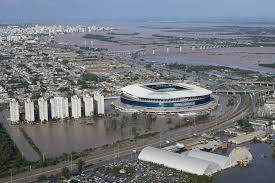
\includegraphics[width=1\linewidth]{flood_rs_02.jpg}
            \caption{Gremio's Stadium vicinity. \\ \textcolor{blue}{Source}: Andre Penner.}
            \label{fig:flood2}
        \end{figure}
    \end{column}

    \begin{column}{0.5\textwidth}
        \begin{figure}
            \centering
            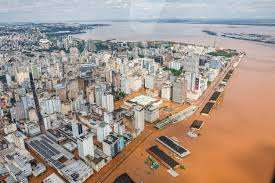
\includegraphics[width=1\linewidth]{flood_rs_03.jpg}
            \caption{Porto Alegre's Historical Center Region. \\ \textcolor{blue}{Source}: Ricardo Stuckert.}
            \label{fig:flood3}
        \end{figure}
    \end{column}
\end{columns}
\end{frame}





\section{Graph and Dataset}

\subsection{Graph Structure}

\begin{frame}{Graph of INMET stations}
\begin{columns}[T,onlytextwidth]
    \begin{column}{0.48\textwidth}
        \begin{figure}
            \centering
            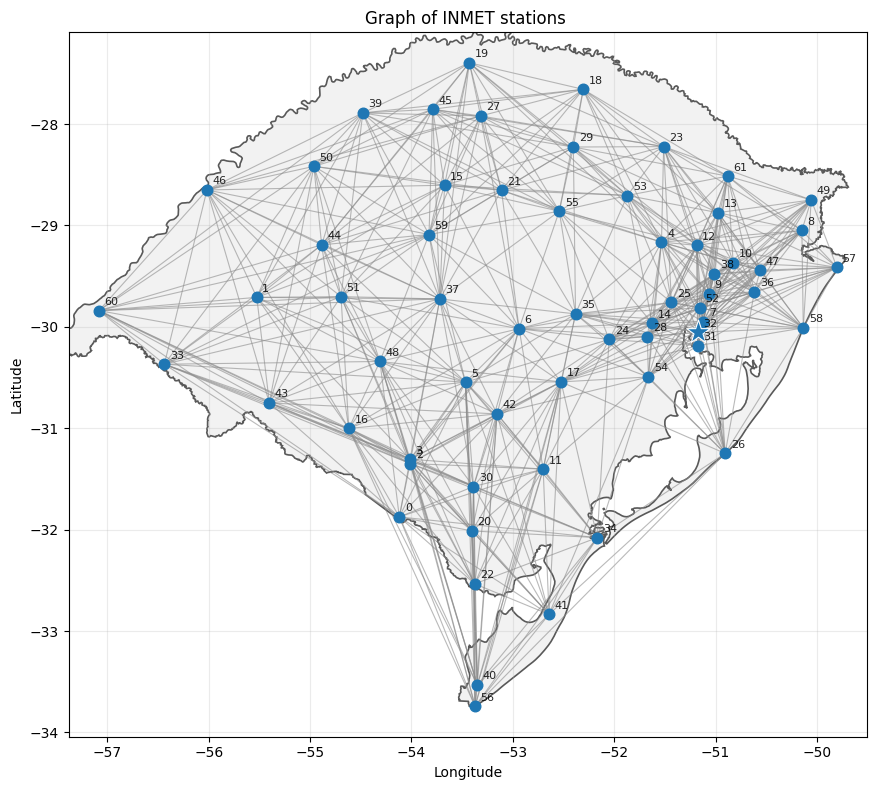
\includegraphics[width=0.83\linewidth]{k_15.png}
            \caption{Graph kNN for $k=15$.}
            \label{fig:knn_15}
        \end{figure}
    \end{column}

    \begin{column}{0.48\textwidth}
        \begin{itemize}
            \item Graph with $61$ nodes constructed from INMET stations locations
            \item Edges created based on the $15$ Nearest Neighbors (kNN)
            \item Each node contains meteorological variables with a temporal resolution of one day
        \end{itemize}
    \end{column}
\end{columns}
\end{frame}



\subsection{Dataset}
\begin{frame}{Datasets}

\begin{itemize}

    \item \textbf{Data used for training}
    \begin{itemize}
        \item ERA5 Dataset (ECMWF)
        \item Daily meteorological data at locations corresponding to INMET weather stations
        \item Dataset period: 01-01-2000 -- 31-12-2025
    \end{itemize}
    \pause

    \vspace{0.3cm}

    \item \textbf{Meteorological Variables}
    \begin{itemize}
        \item Daily precipitation (target variable)
        \item Temperature and dew point at sea level (feature)
        \item Specific humidity (feature)
        \item Vertical velocity at three atmospheric levels (feature)
    \end{itemize}
    \pause

    \vspace{0.3cm}

    \item \textbf{Data Processing}
    \begin{itemize}
        \item Daily aggregation using mean, maximum, and minimum values
        \item Features normalized using z-score normalization
        \item Grouping into temporal windows
    \end{itemize}

\end{itemize}
\vfill
{\scriptsize Source: Copernicus Climate Change Service, Climate Data Store, (2023): ERA5 hourly data on single levels from 1940 to present.}

\end{frame}

\begin{frame}

\begin{columns}[T,onlytextwidth]
\begin{column}{0.30\textwidth}
    \begin{block}{Features per station}
    \scriptsize
    \begin{itemize}
        \setlength{\itemsep}{2pt}
        \item \textbf{25 features per day}
        \item Precipitation: 1
        \item Temperature + dew point: 6\\
              (mean, min, max)
        \item Specific humidity: 6\\
              (1000 and 850 hPa)
        \item Vertical velocity: 12\\
              (300, 500 and 850 hPa)
        \item Input of $15$ consecutive days and target of $5$ future precipitation values
    \end{itemize}
    \end{block}

    \vspace{0.15cm}
    \centering
    \scriptsize
    \(\mathbf{x}_t^{(i)} \in \mathbb{R}^{25}\)\\[2pt]
    \(X \in \mathbb{R}^{15\times 61 \times25}\)\\
    \(Y \in \mathbb{R}^{5\times 61}\)
\end{column}
\pause
\hfill
\begin{column}{0.66\textwidth}
\centering
\resizebox{\linewidth}{!}{%
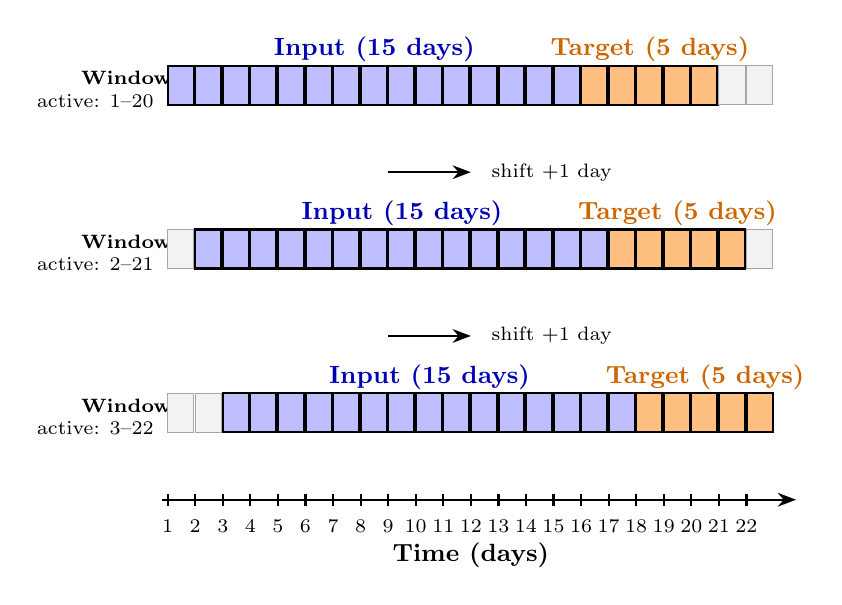
\begin{tikzpicture}[x=0.35cm,y=0.52cm,>=Stealth]

% -------------------------
% Parâmetros
% -------------------------
\def\boxsize{0.95}     % lado dos quadrados
\def\inputlen{15}
\def\targetlen{5}
\def\totallen{20}



% -------------------------
% Janelas
% -------------------------
\drawalignedwindow{8}{1}{1}
\drawalignedwindow{4}{2}{2}
\drawalignedwindow{0}{3}{3}

% -------------------------
% Setas de deslocamento
% -------------------------
\draw[->, thick] (8.0,6.35) -- (11.0,6.35);
\node[anchor=west, font=\scriptsize] at (11.4,6.35) {shift +1 day};

\draw[->, thick] (8.0,2.35) -- (11.0,2.35);
\node[anchor=west, font=\scriptsize] at (11.4,2.35) {shift +1 day};

% -------------------------
% Eixo do tempo
% -------------------------
\draw[->, thick] (-0.2,-1.65) -- (22.8,-1.65);
\foreach \i in {1,...,22} {
    \draw[thick] (\i-1,-1.80) -- (\i-1,-1.50);
    \node[anchor=north, font=\scriptsize] at (\i-1,-1.90) {\i};
}
\node[font=\bfseries\small] at (11,-3.00) {Time (days)};

\end{tikzpicture}
}%
\captionof{figure}{Sliding Window construction from timeseries data.}
\end{column}
\end{columns}
  
\end{frame}

\section{GNN+LSTM Model}

\subsection{Model architecture}



\begin{frame}{GLSTM architecture}
   
\begin{columns}[c]
\column{0.60\textwidth}
    \begin{figure}
        \centering
        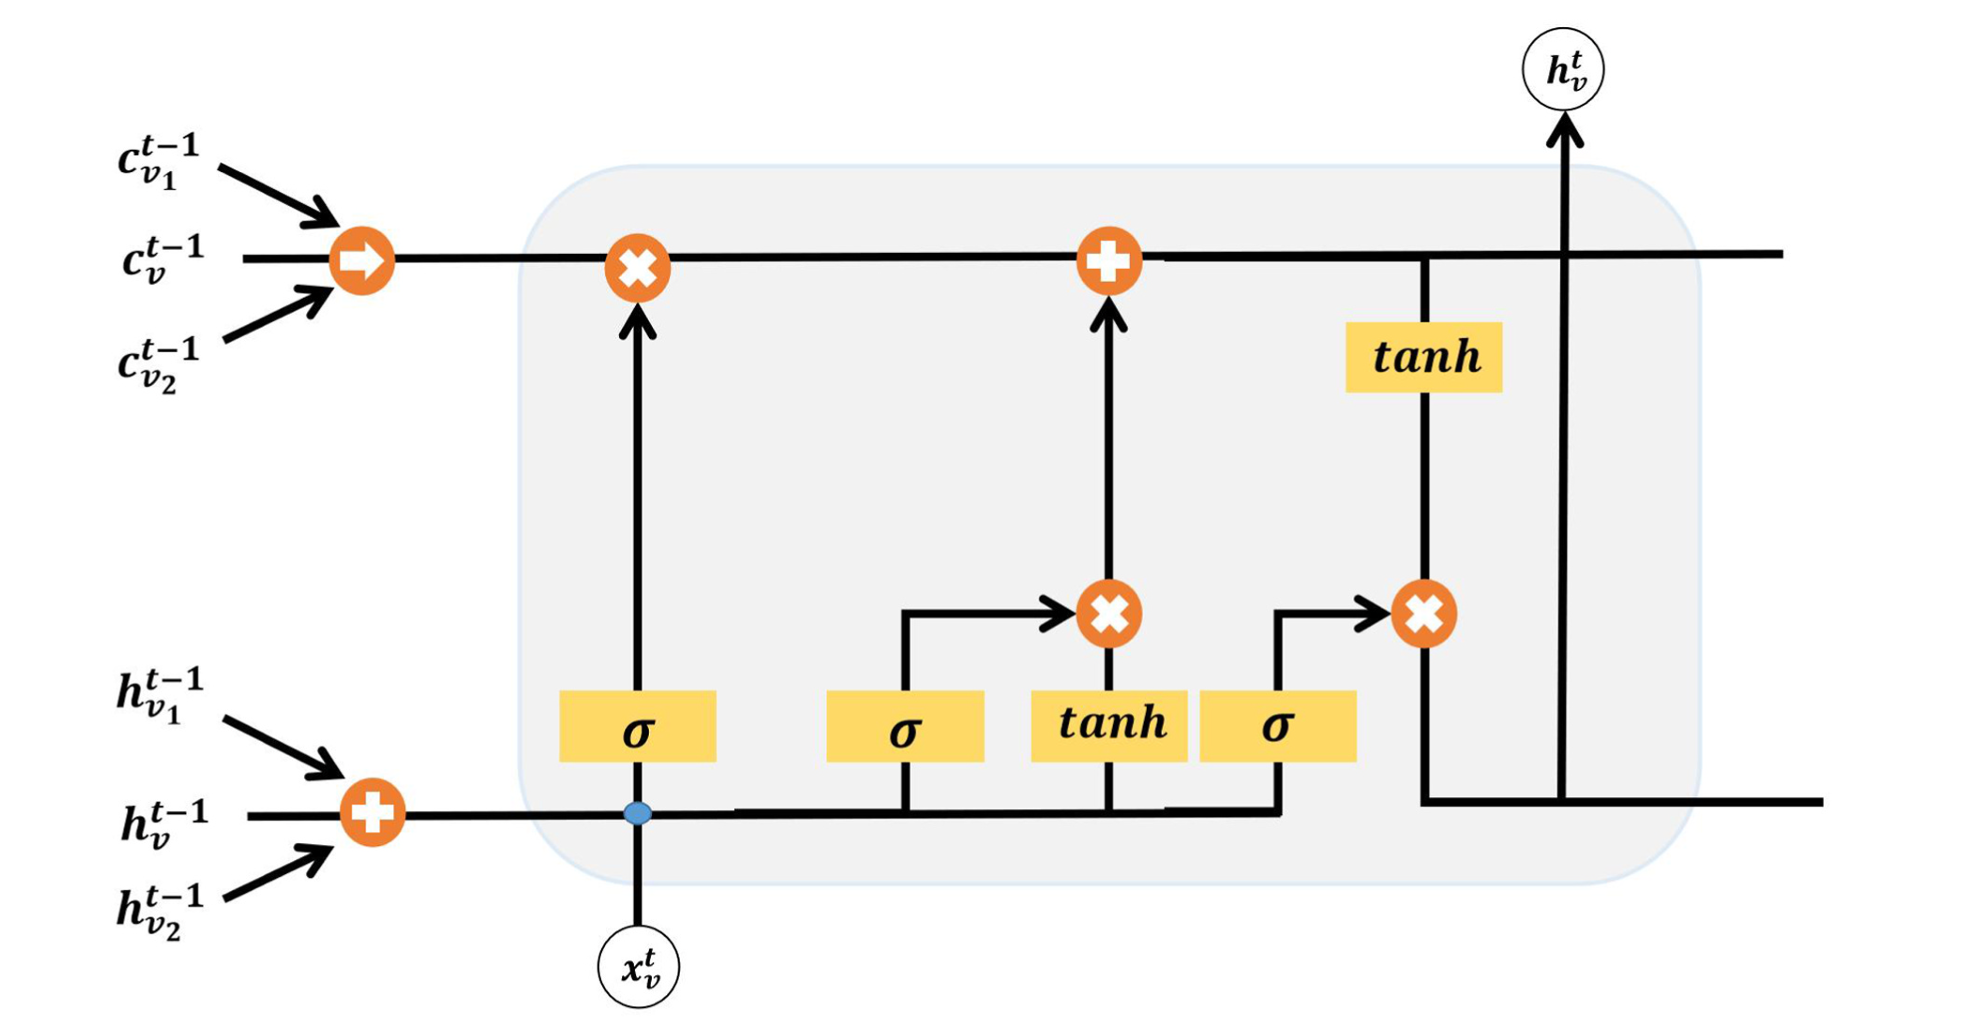
\includegraphics[width=1\linewidth]{GLSTM_block_fig.png}
        \caption{GLSTM layer architecture. \\ \textcolor{blue}{Source}: Gao and Li (2021).}
        \label{fig:glstm_arc}
    \end{figure}
    \column{0.4\textwidth}\hfill


    \begin{align*}
        I_t &= \sigma (W^{i}X_t+U^{i}H_{t-1}\textcolor{red}{W_{adj}}+B^{i}) \\
        F_t &= \sigma (W^{f}X_t+U^{f}H_{t-1}+B^{f}) \\
        O_t &= \sigma (W^{O}X_t+U^{O}H_{t-1}\textcolor{red}{W_{adj}}+B^{O}) \\
        U_t &=  tanh(W^{u}X_t+U^{u}H_{t-1}\textcolor{red}{W_{adj}}+B^{u}) \\
        C_t &= I_t \circ U_t + F_t \circ C_{t-1}\textcolor{red}{W_{adj}} \\
        H_t &= O_t \circ tanh(C_t)
    \end{align*}

\end{columns}
\end{frame}

\begin{frame}{GLTM architecture}
\begin{figure}
        \centering
        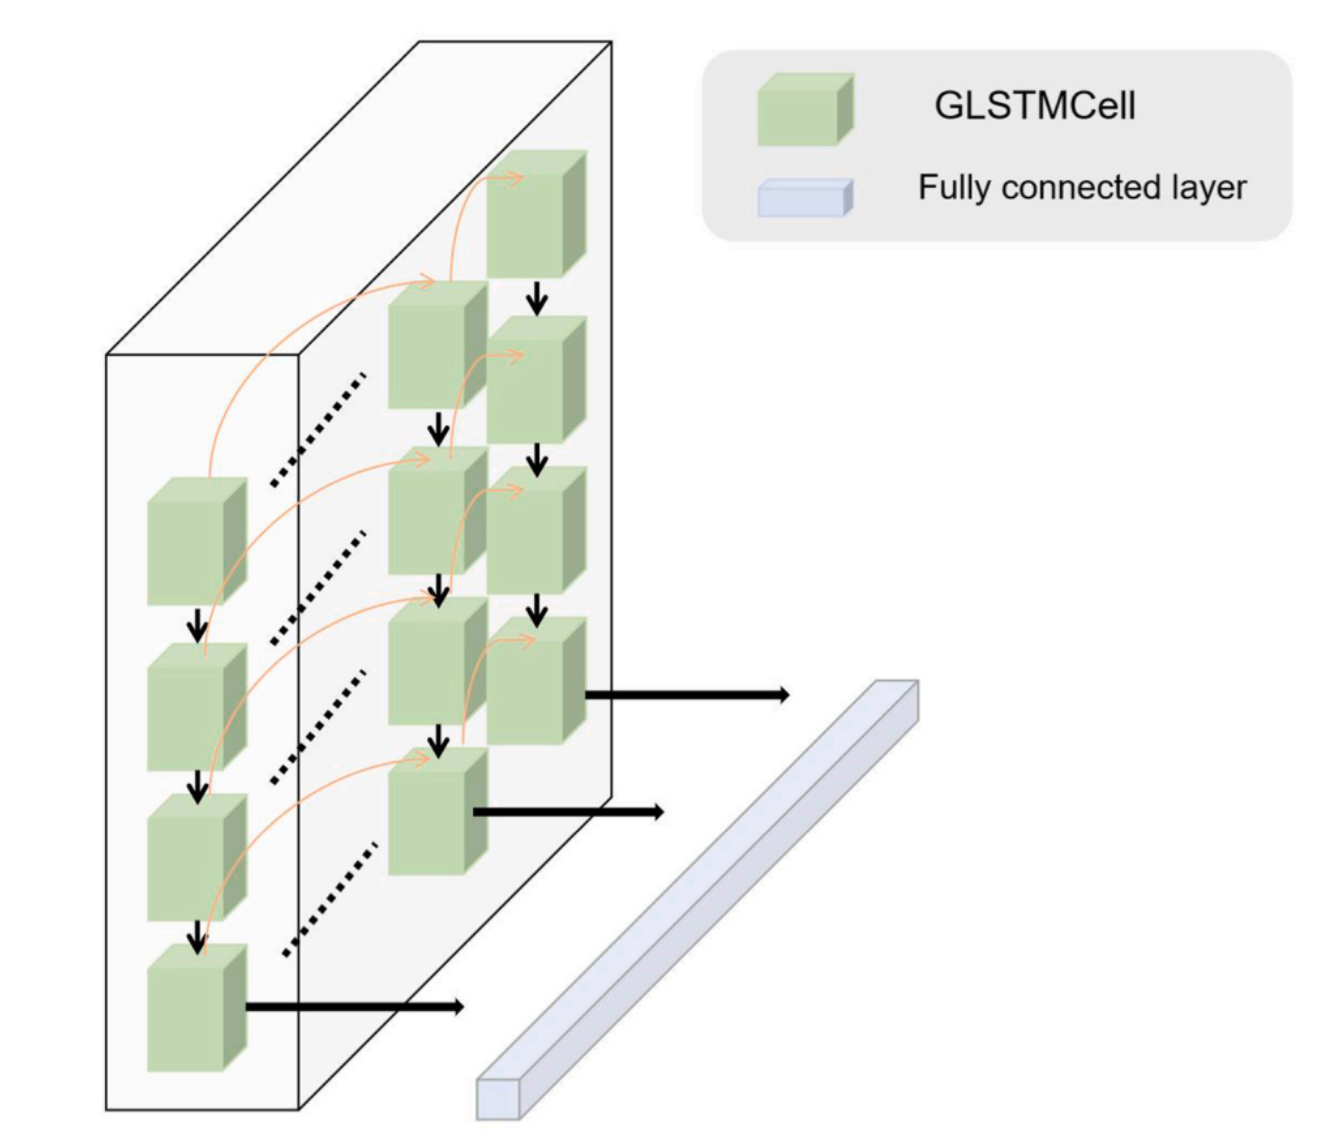
\includegraphics[width=0.5\linewidth]{glstm_arc.png}
        \caption{GLSTM layer architecture. \\ \textcolor{blue}{Source}: Gao and Li (2021).}
        \label{fig:glstm_arc_2}
    \end{figure}
\end{frame}





\section{Results}

\subsection{Parameter and loss function}

\begin{frame}{Model Parameters and Loss Function}

\begin{columns}[T]

%--------------------------------
\begin{column}{0.47\textwidth}

\textbf{Model Parameters}

\begin{itemize}
    \item \textbf{Graph layer:} Spatial-Convolution
    \item \textbf{LSTM hidden size:} 256
    \item \textbf{LSTM layers:} 2
    \item \textbf{Dropout:} 0.3
    \item \textbf{Optimizer:} AdamW
    \item \textbf{Learning rate:} $10^{-3}$
    \item \textbf{Batch size:} 8
    \item \textbf{Weight decay:} $1\times10^{-4}$
\end{itemize}

\end{column}

%--------------------------------
\begin{column}{0.47\textwidth}

\textbf{Loss Function}

\vspace{0.3cm}

\begin{itemize}
    \item \textbf{Loss function:} quantile mse loss
\end{itemize}

\begin{center}
\resizebox{\linewidth}{!}{$\displaystyle
\mathcal{L}_{q}(y,\hat{y})
=
\begin{cases}
w_{1}(y-\hat{y})^2, & y > Q_{0.9},\\[2mm]
w_2(y-\hat{y})^2, & y \in [Q_{0.5}, Q_{0.9}], \\[2mm]
w_{1-q}(y-\hat{y})^2, & y<Q_{0.5}
\end{cases}
 $}
\end{center}


\vspace{0.3cm}

\begin{itemize}
    \item Asymmetric MSE controlled by quantile $q$
    \item Penalizes more the loss in extreme points in the target variable
\end{itemize}

\end{column}

\end{columns}

\end{frame}



\subsection{Results and discussion}

\begin{frame}{Results and Discussion}
\begin{table}[H]
\centering
\small
\begin{tabular}{l r r r r}
\toprule
Hidden dim & RMSE & MAE & $R^2$ \\
\midrule
256 & \textbf{11.81} & \textbf{8.045} & \textbf{-0.5779} \\
512 & 12.11 & 8.46 & -0.6608 \\
1024 & 12.12 & 10.45 & -0.6629 \\
\bottomrule
\end{tabular}
\caption{Metrics on test data with all lead days combined.}
\end{table}
        
\end{frame}

\begin{frame}{Predition analysis}

\begin{columns}[c]
        \column{0.48\textwidth}
        \centering
        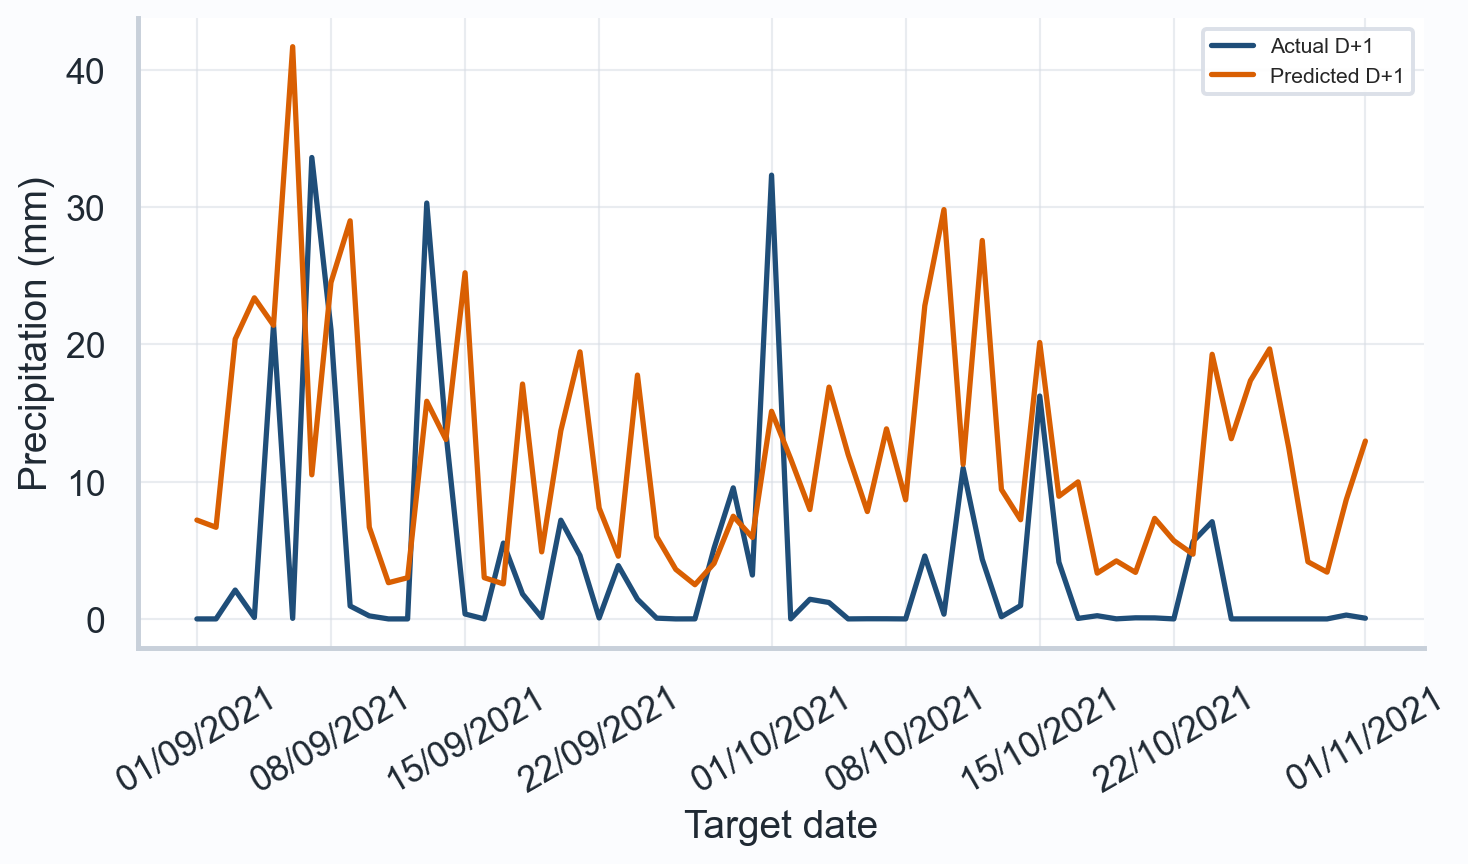
\includegraphics[width=0.7\linewidth]{plots_presentation/porto_alegre_true_vs_predicted_lead_day_01_20210901_20211101.png}
        \captionof{figure}{Prediction for lead day 1.}

        \column{0.48\textwidth}
        \centering
        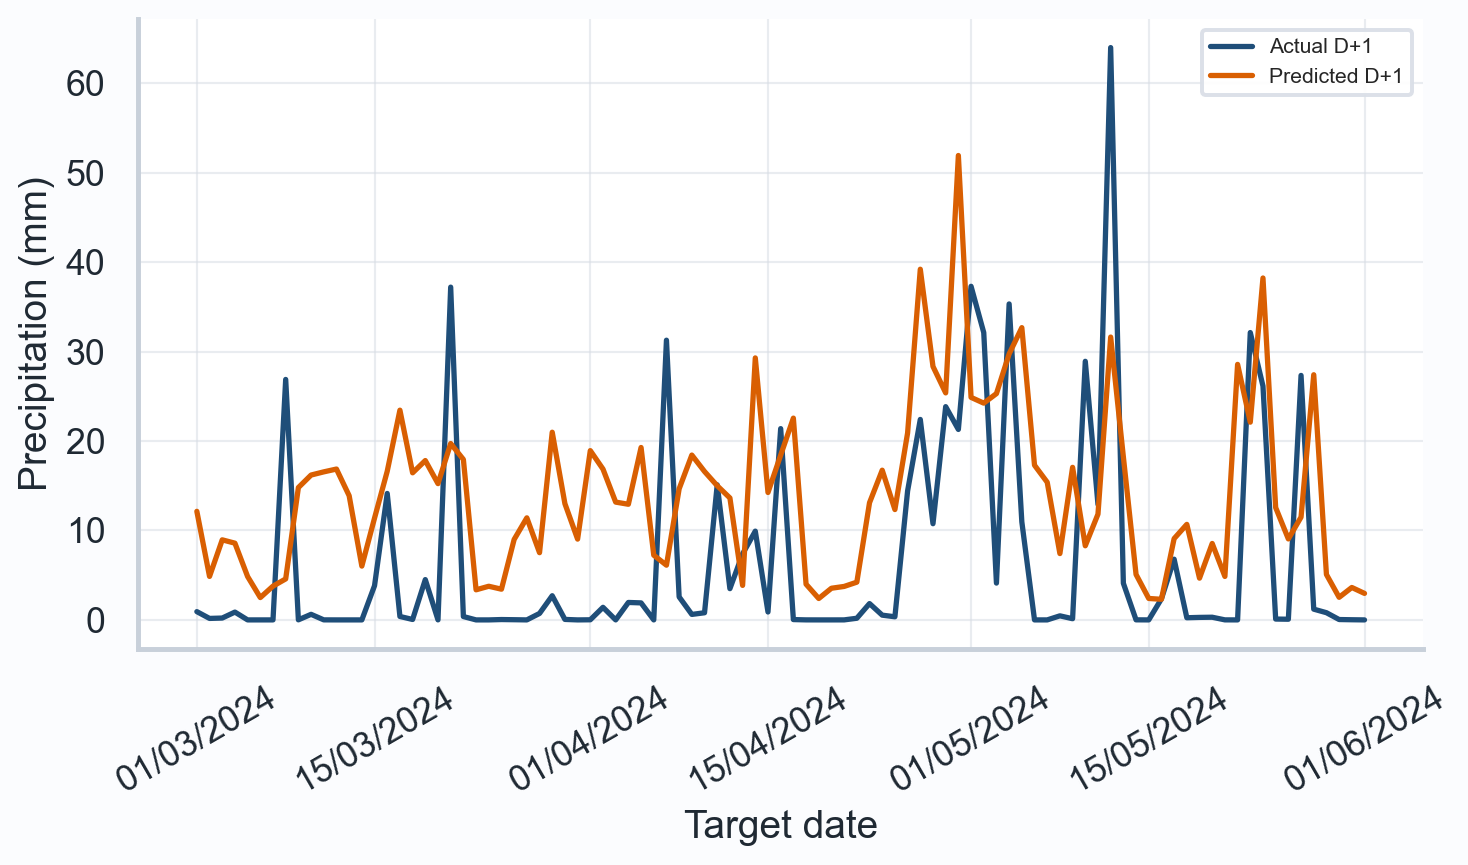
\includegraphics[width=0.7\linewidth]{plots_presentation/porto_alegre_true_vs_predicted_lead_day_01_20240301_20240601.png}
        \captionof{figure}{Prediction for lead day 1.}
    \end{columns}

    \begin{columns}[c]
        \column{0.48\textwidth}
        \centering
        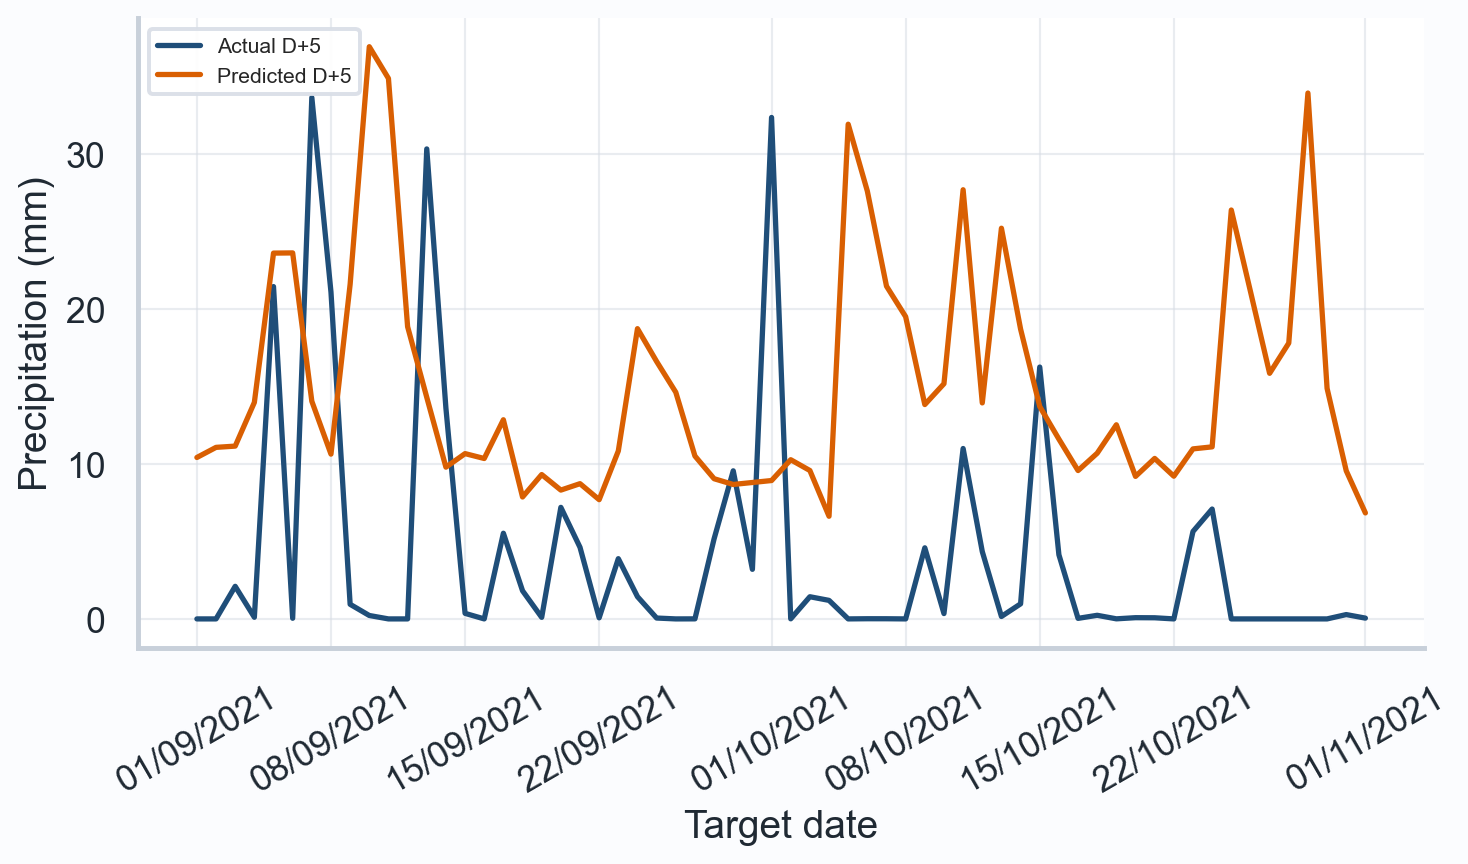
\includegraphics[width=0.7\linewidth]{plots_presentation/porto_alegre_true_vs_predicted_lead_day_05_20210901_20211101.png}
        \captionof{figure}{Prediction for lead day 5.}

        \column{0.48\textwidth}
        \centering
        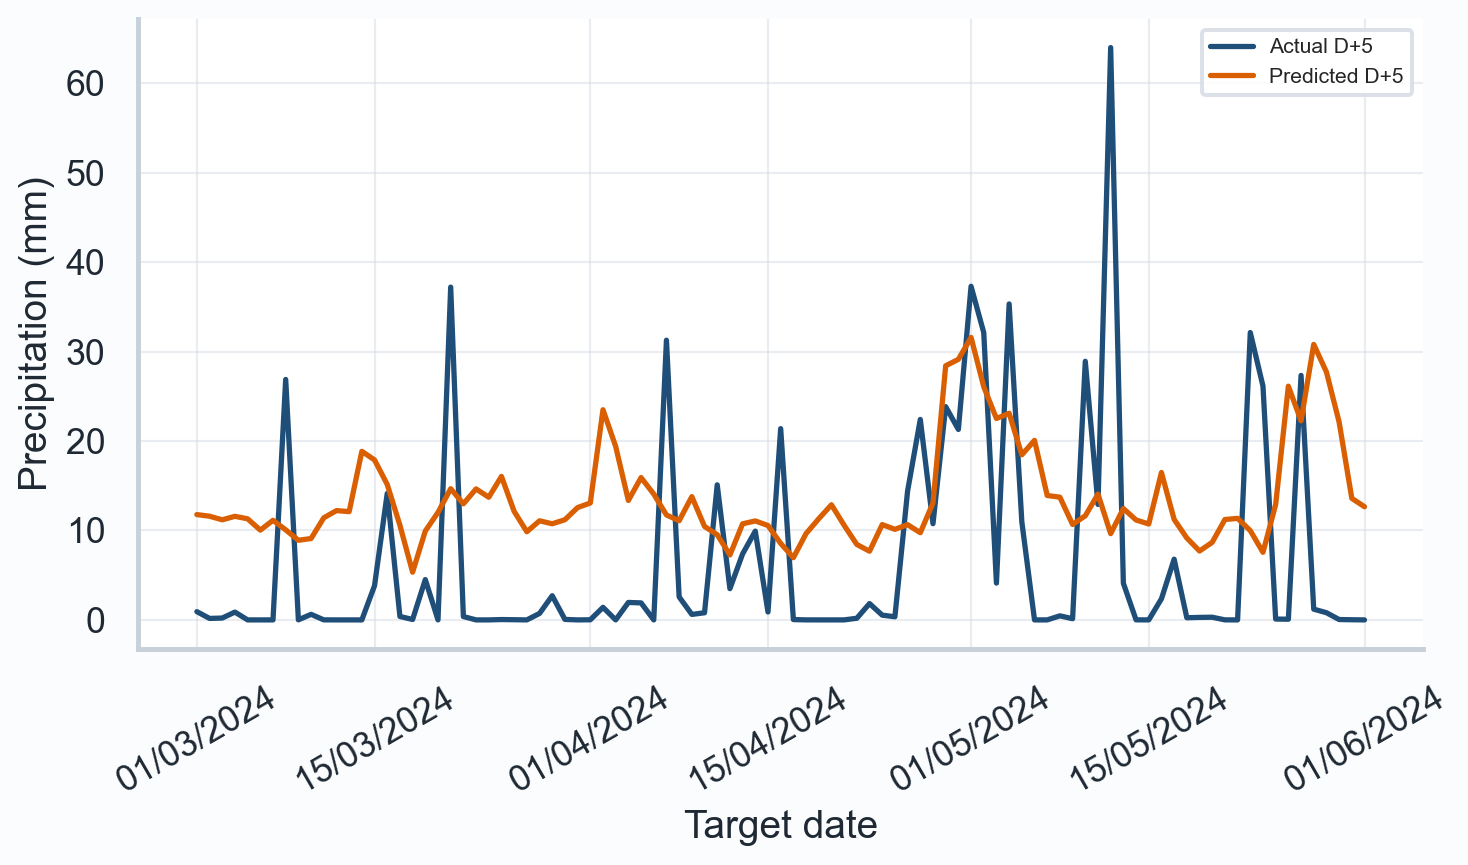
\includegraphics[width=0.7\linewidth]{plots_presentation/porto_alegre_true_vs_predicted_lead_day_05_20240301_20240601.png}
        \captionof{figure}{Prediction for lead day 5.}
    \end{columns}


\end{frame}

\begin{frame}{Animated Prediction vs Real}
\centering
\begin{minipage}{0.86\linewidth}
\centering
\begin{animateinline}[
  label=rsrain,
  poster=first,
  autoplay,
  autopause,
  autoresume,
  loop,
  controls=all,
  controlsaligned=center
]{2}
  \makebox[\linewidth][c]{%
    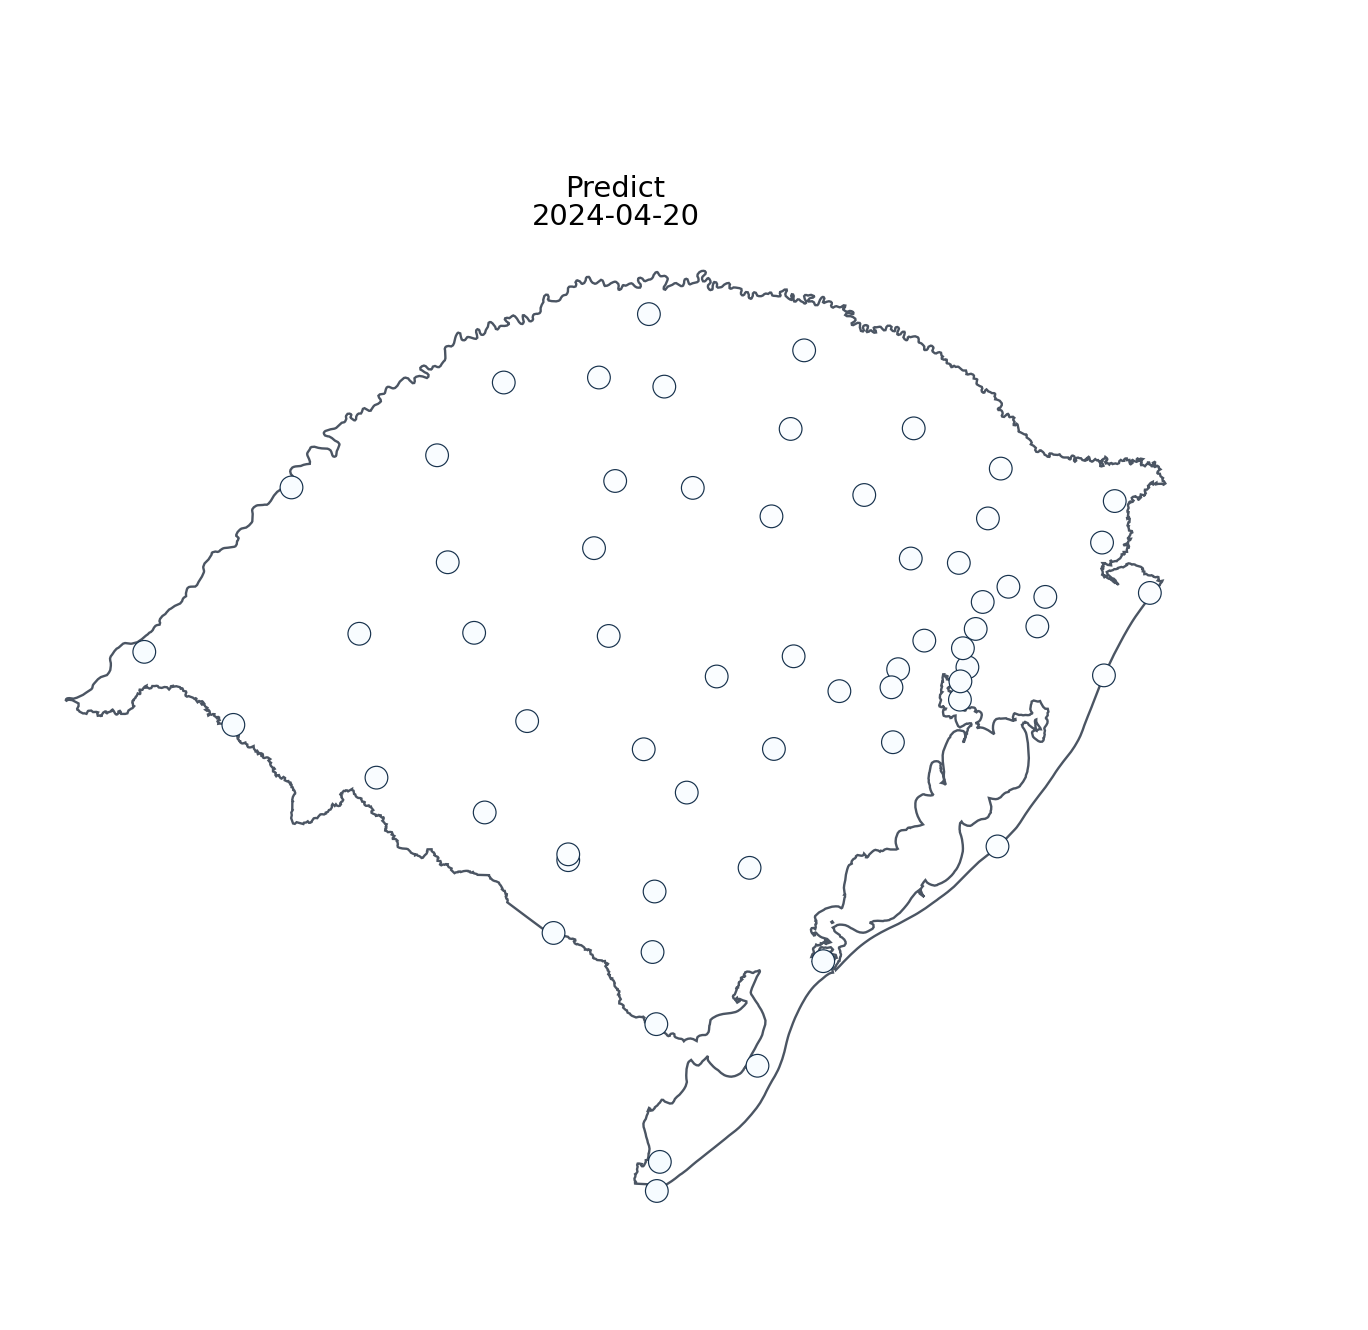
\includegraphics[width=0.48\linewidth]{Predict/frame_001.png}\hfill
    
\includegraphics[width=0.48\linewidth]{Real/frame_001.png}%
  }
  \newframe
  \makebox[\linewidth][c]{%
    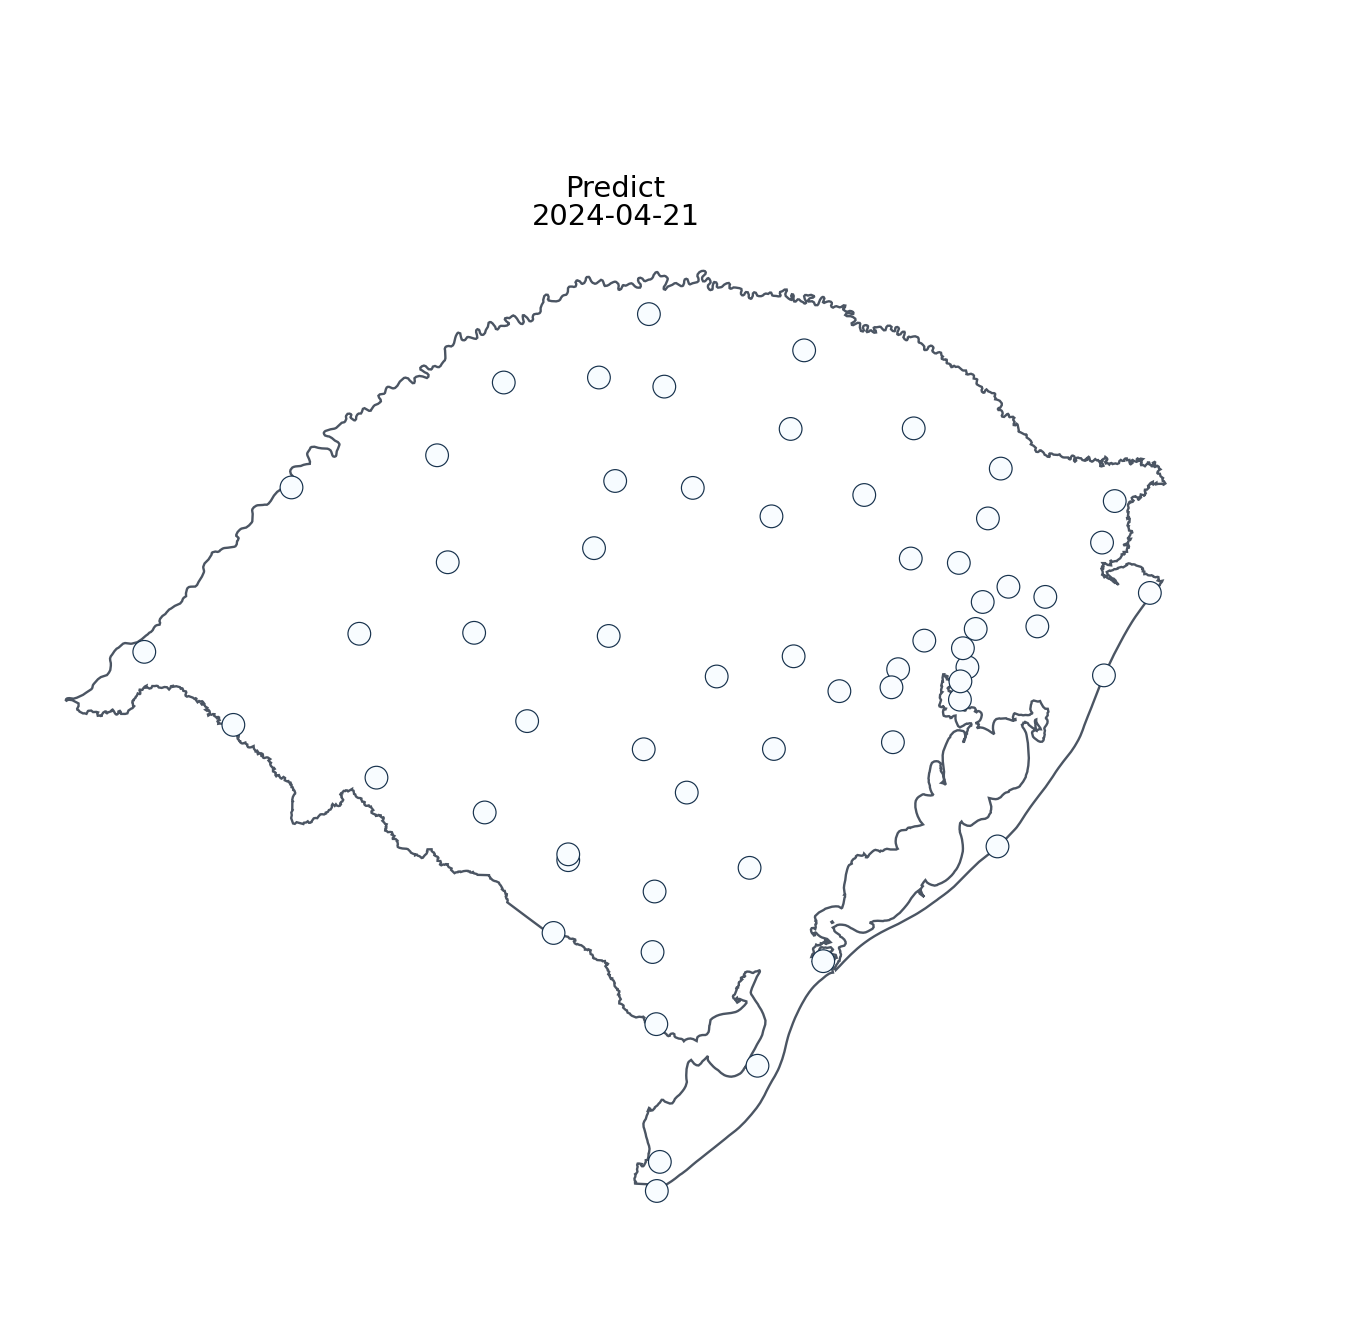
\includegraphics[width=0.48\linewidth]{Predict/frame_002.png}\hfill
    
\includegraphics[width=0.48\linewidth]{Real/frame_002.png}%
  }
  \newframe
  \makebox[\linewidth][c]{%
    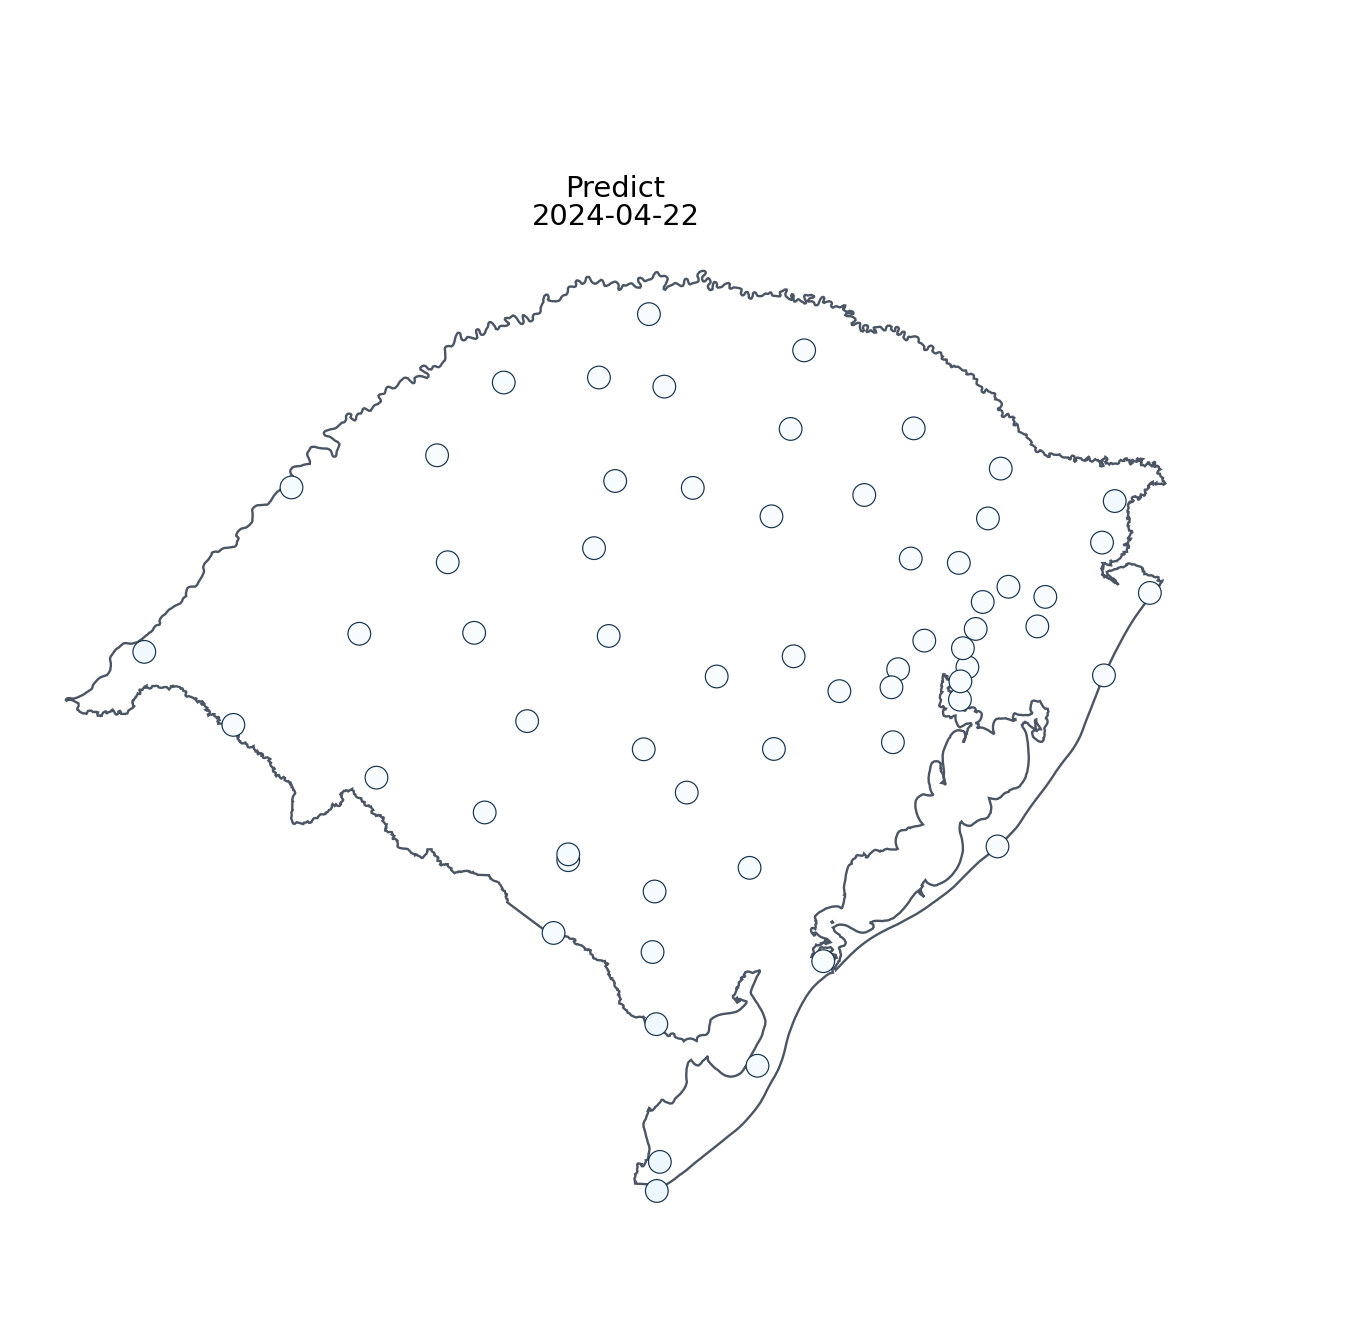
\includegraphics[width=0.48\linewidth]{Predict/frame_003.png}\hfill
    
\includegraphics[width=0.48\linewidth]{Real/frame_003.png}%
  }
  \newframe
  \makebox[\linewidth][c]{%
    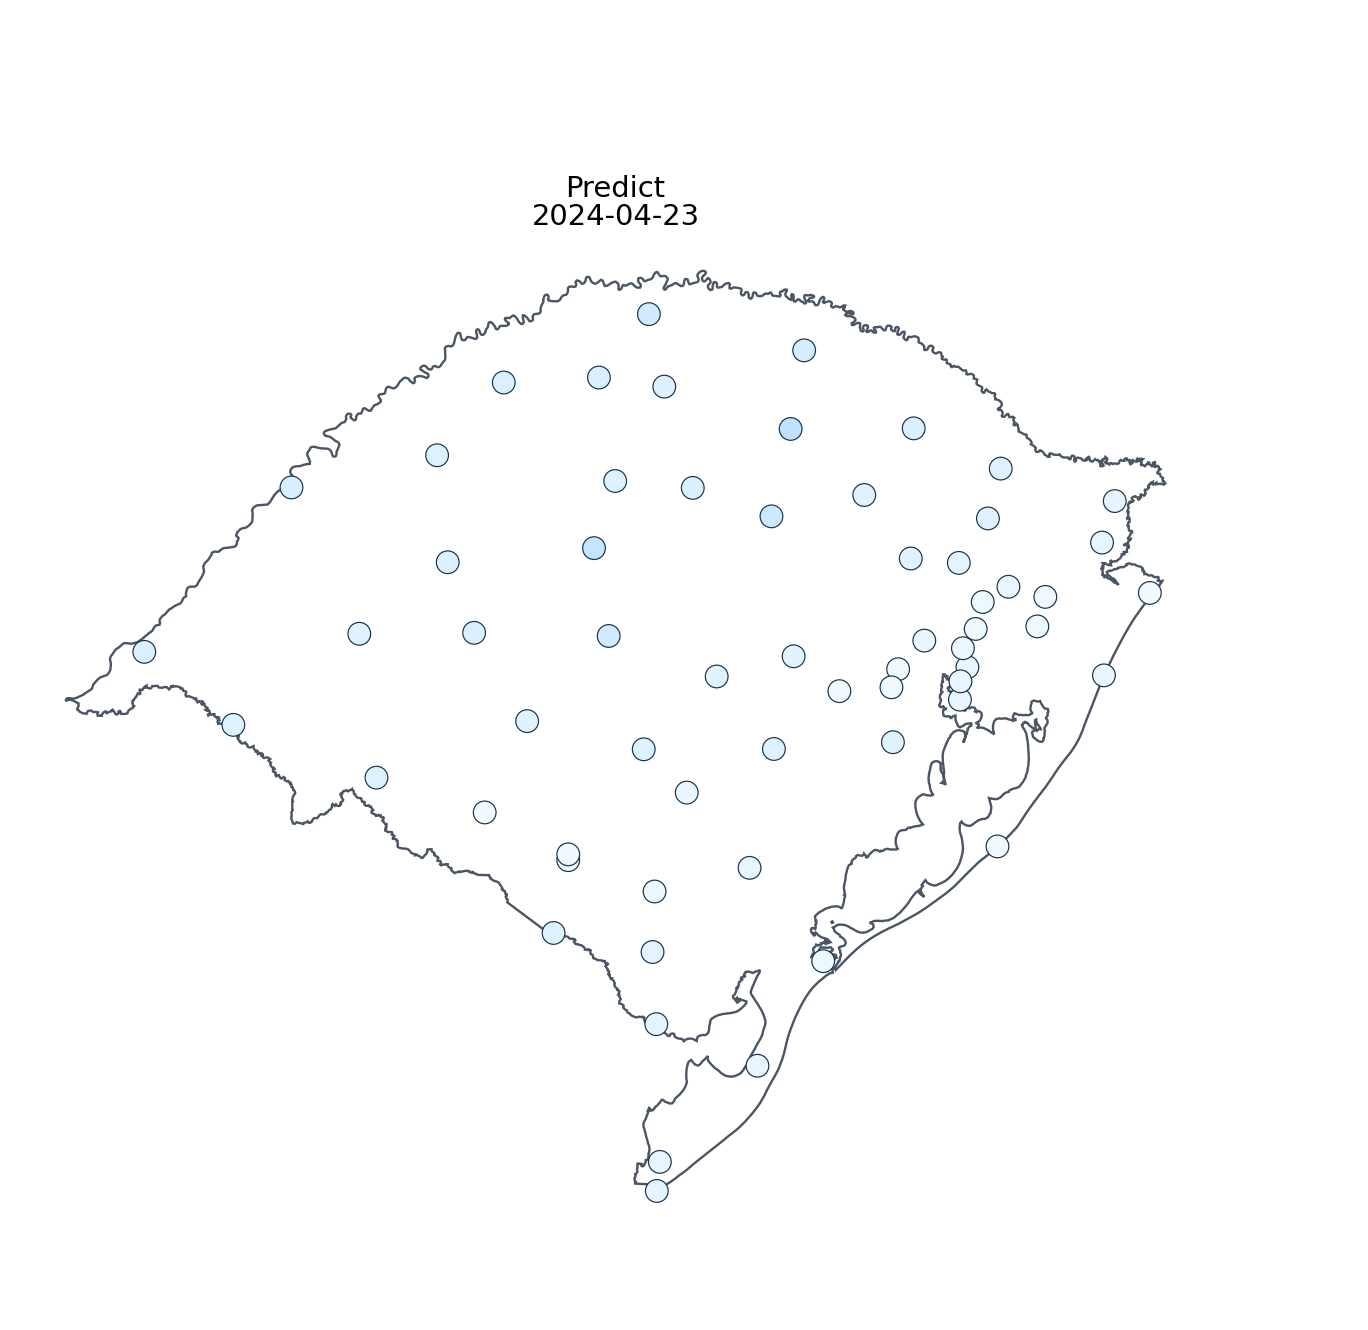
\includegraphics[width=0.48\linewidth]{Predict/frame_004.png}\hfill
    
\includegraphics[width=0.48\linewidth]{Real/frame_004.png}%
  }
  \newframe
  \makebox[\linewidth][c]{%
    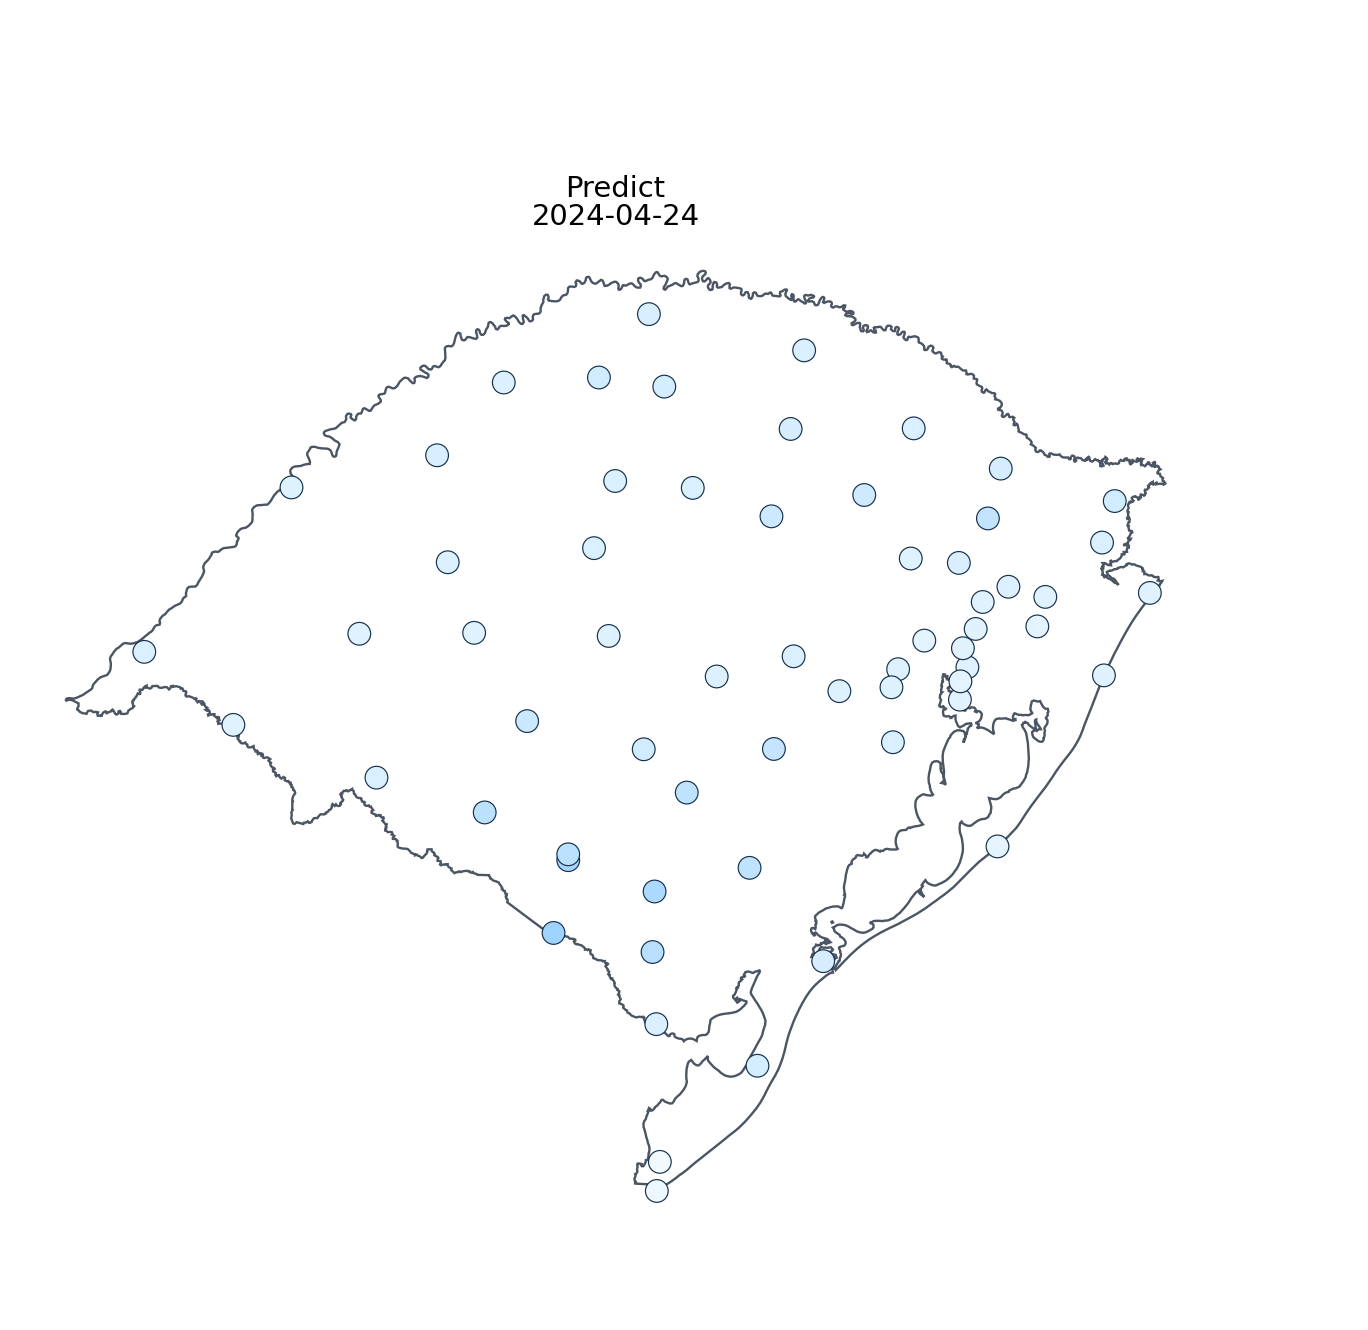
\includegraphics[width=0.48\linewidth]{Predict/frame_005.png}\hfill
    
\includegraphics[width=0.48\linewidth]{Real/frame_005.png}%
  }
  \newframe
  \makebox[\linewidth][c]{%
    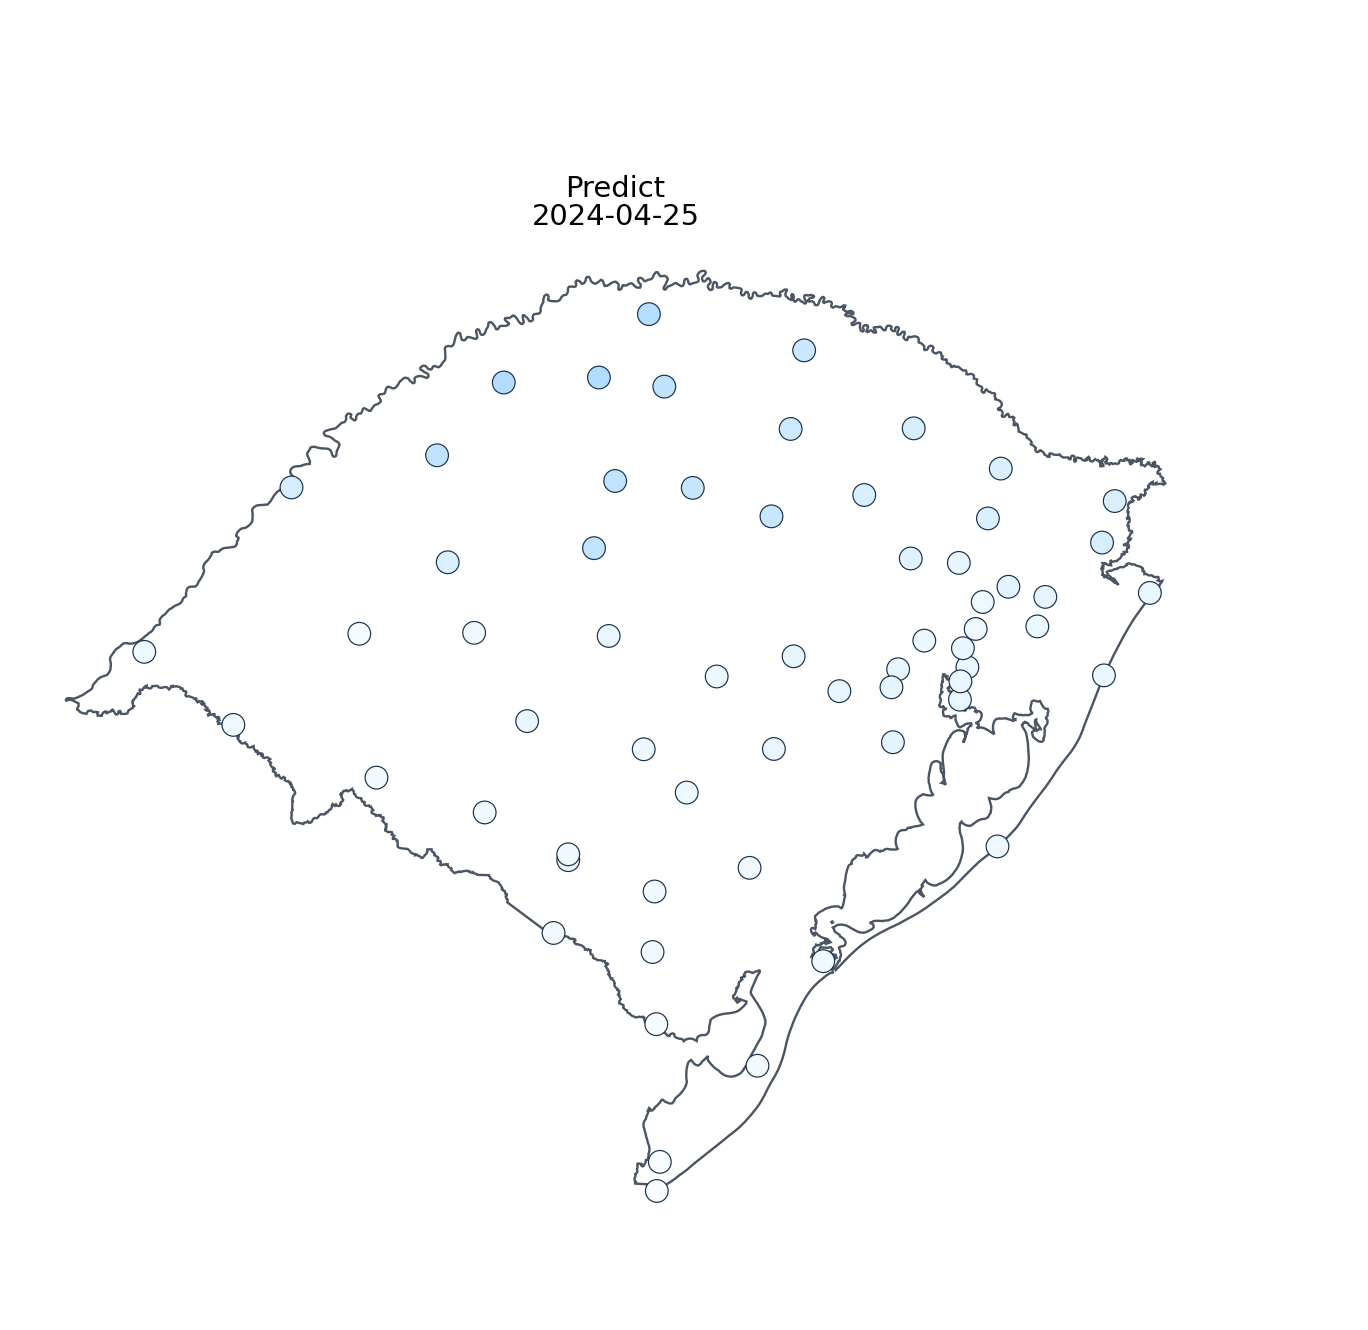
\includegraphics[width=0.48\linewidth]{Predict/frame_006.png}\hfill
    
\includegraphics[width=0.48\linewidth]{Real/frame_006.png}%
  }
  \newframe
  \makebox[\linewidth][c]{%
    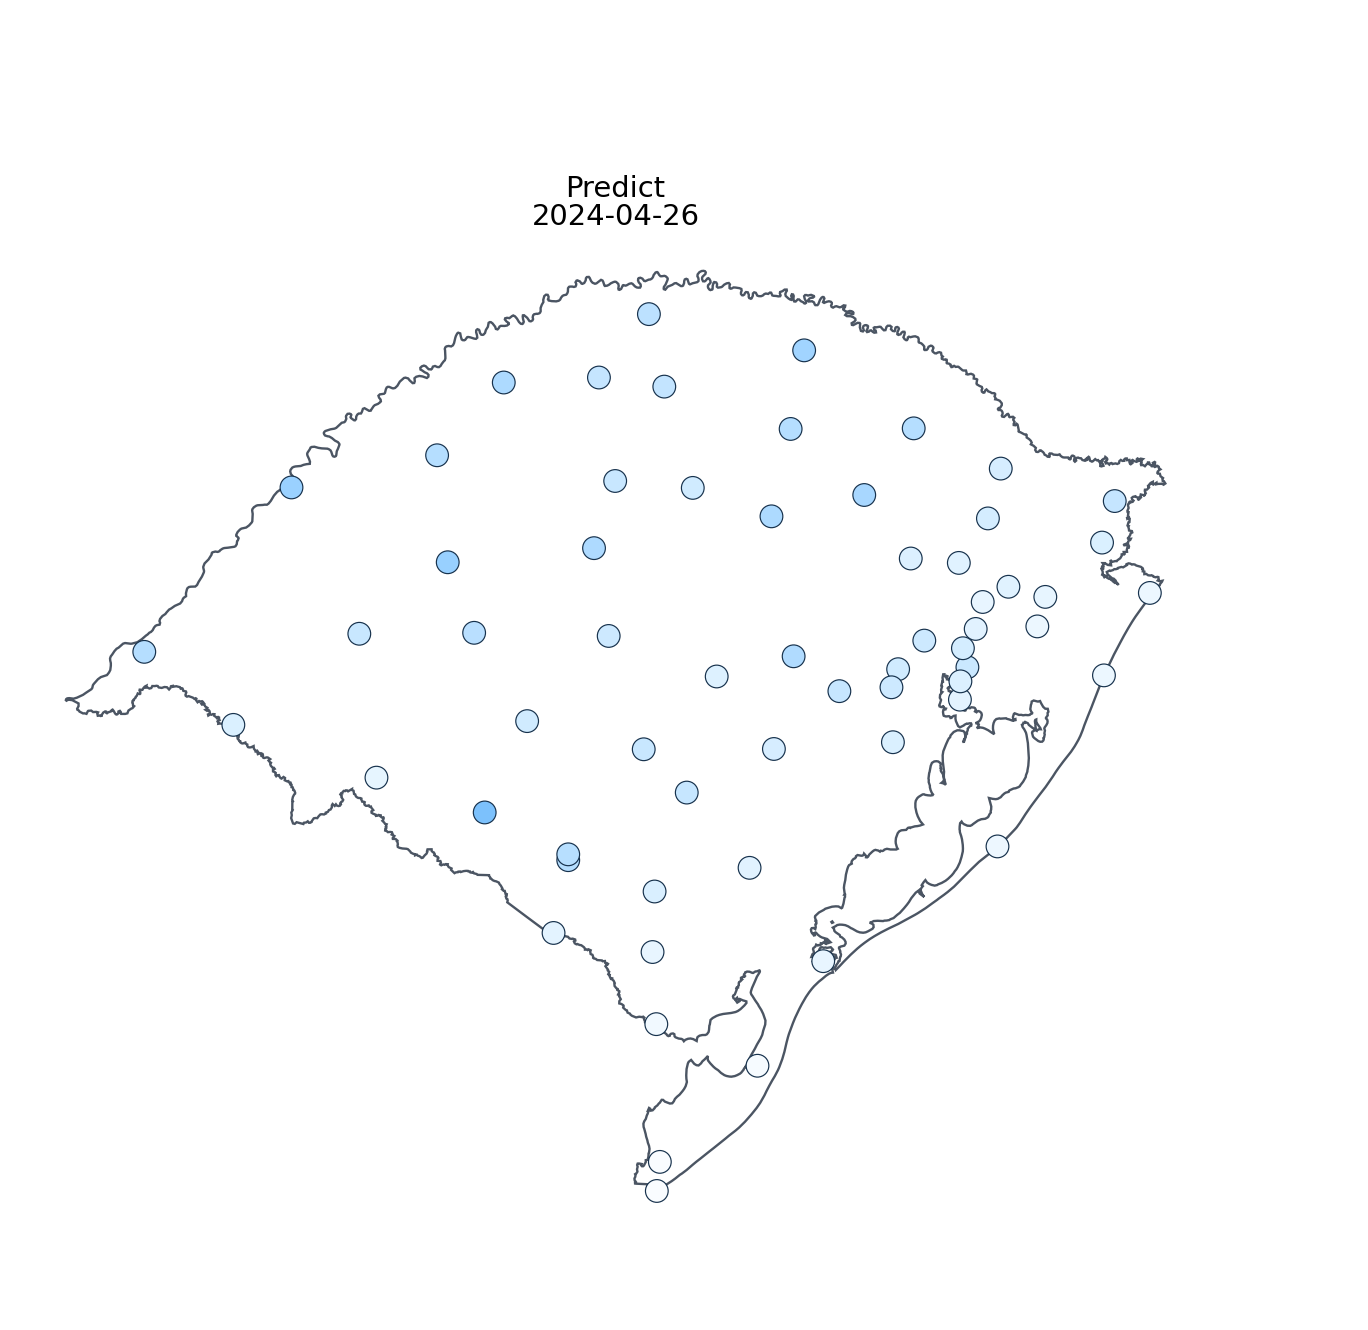
\includegraphics[width=0.48\linewidth]{Predict/frame_007.png}\hfill
    
\includegraphics[width=0.48\linewidth]{Real/frame_007.png}%
  }
  \newframe
  \makebox[\linewidth][c]{%
    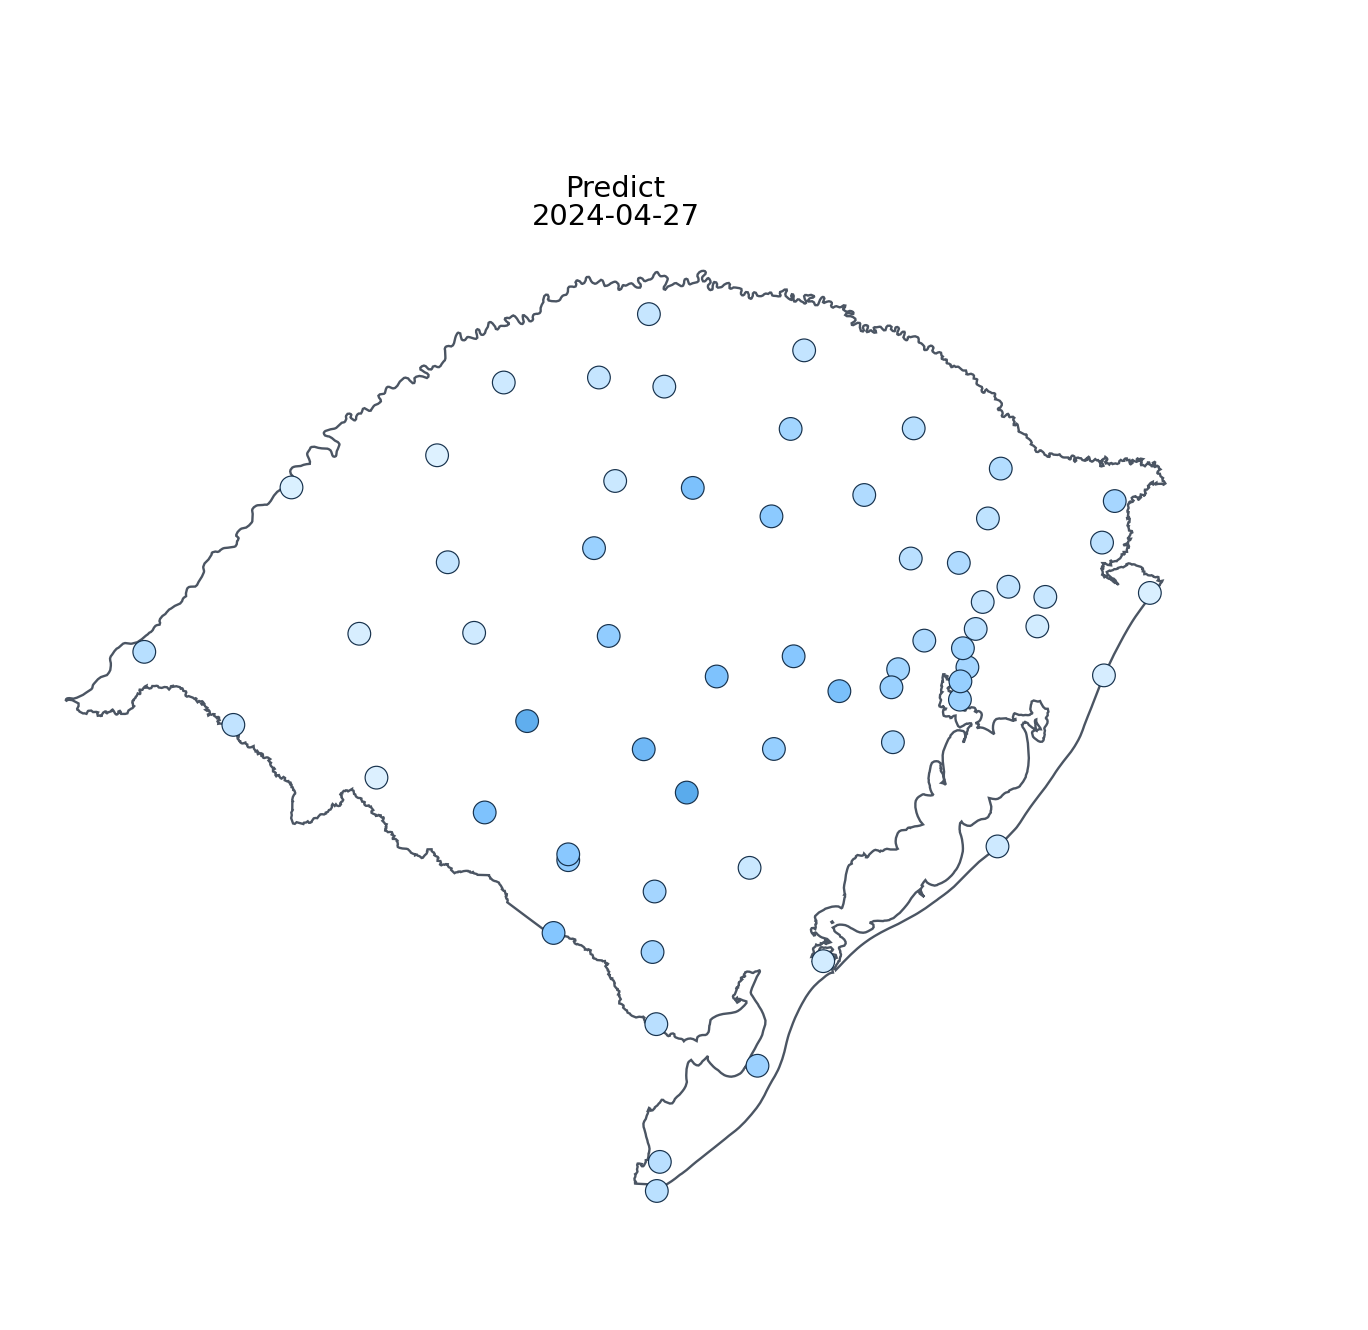
\includegraphics[width=0.48\linewidth]{Predict/frame_008.png}\hfill
    
\includegraphics[width=0.48\linewidth]{Real/frame_008.png}%
  }
  \newframe
  \makebox[\linewidth][c]{%
    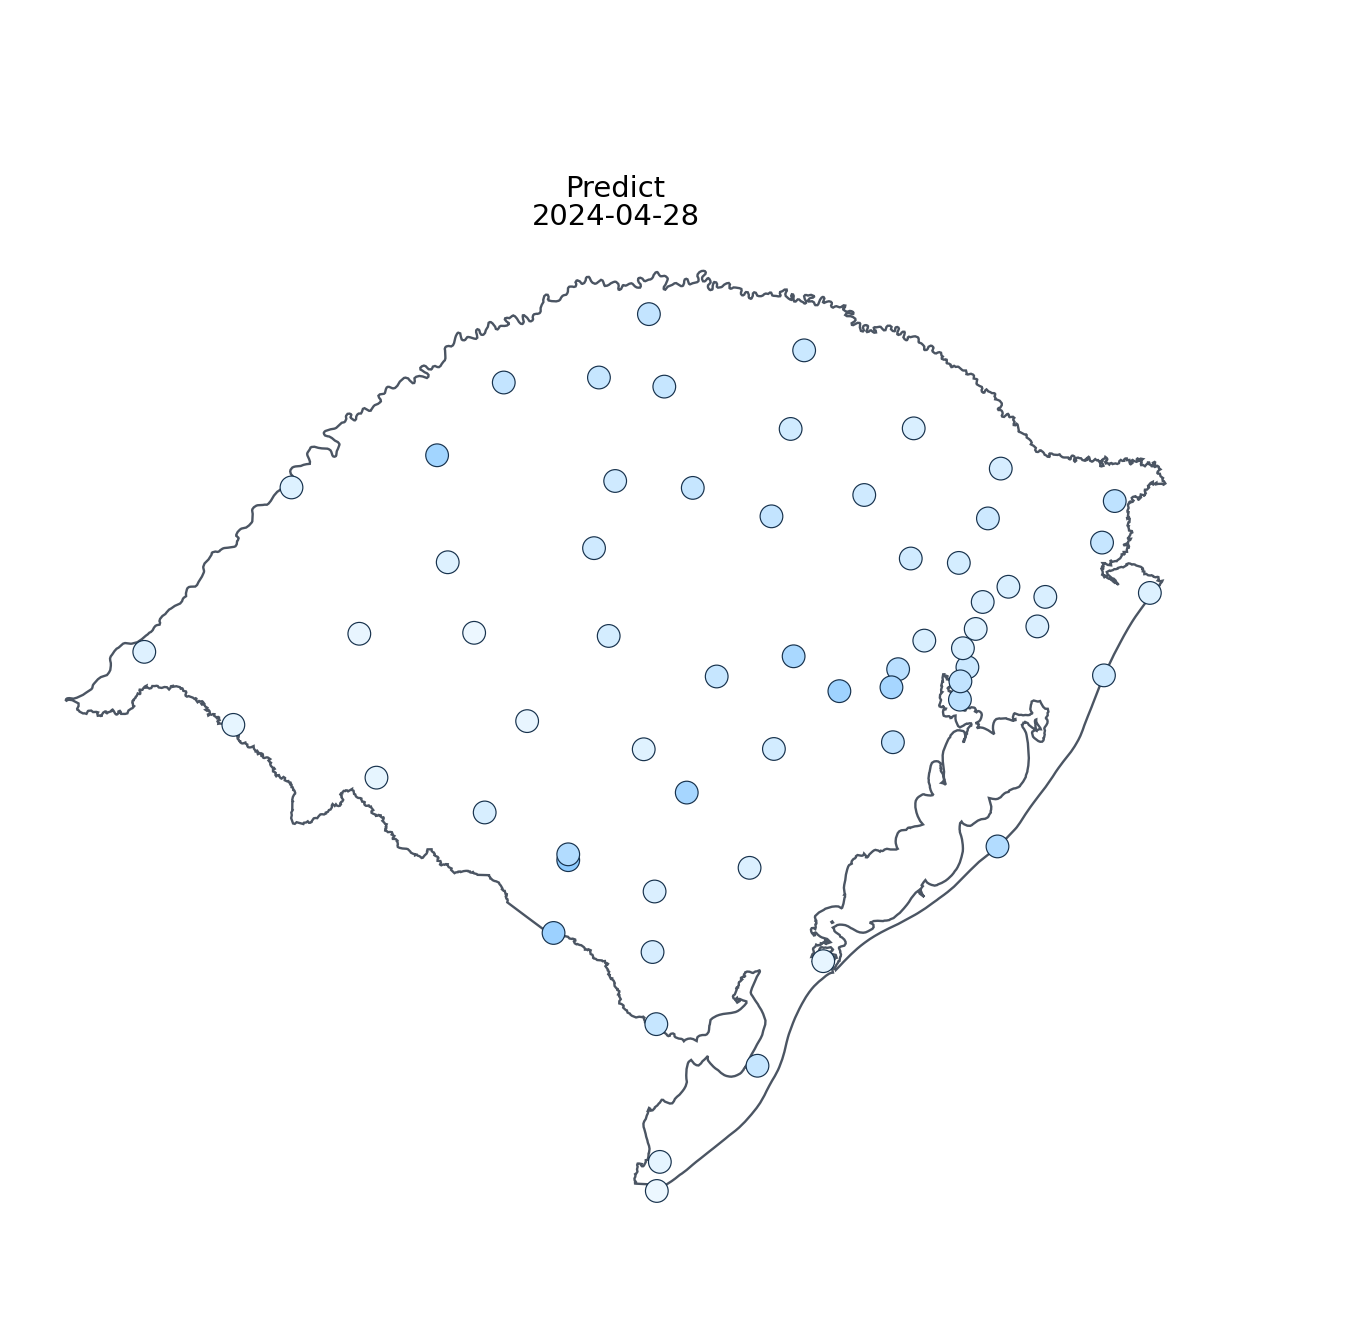
\includegraphics[width=0.48\linewidth]{Predict/frame_009.png}\hfill
    
\includegraphics[width=0.48\linewidth]{Real/frame_009.png}%
  }
  \newframe
  \makebox[\linewidth][c]{%
    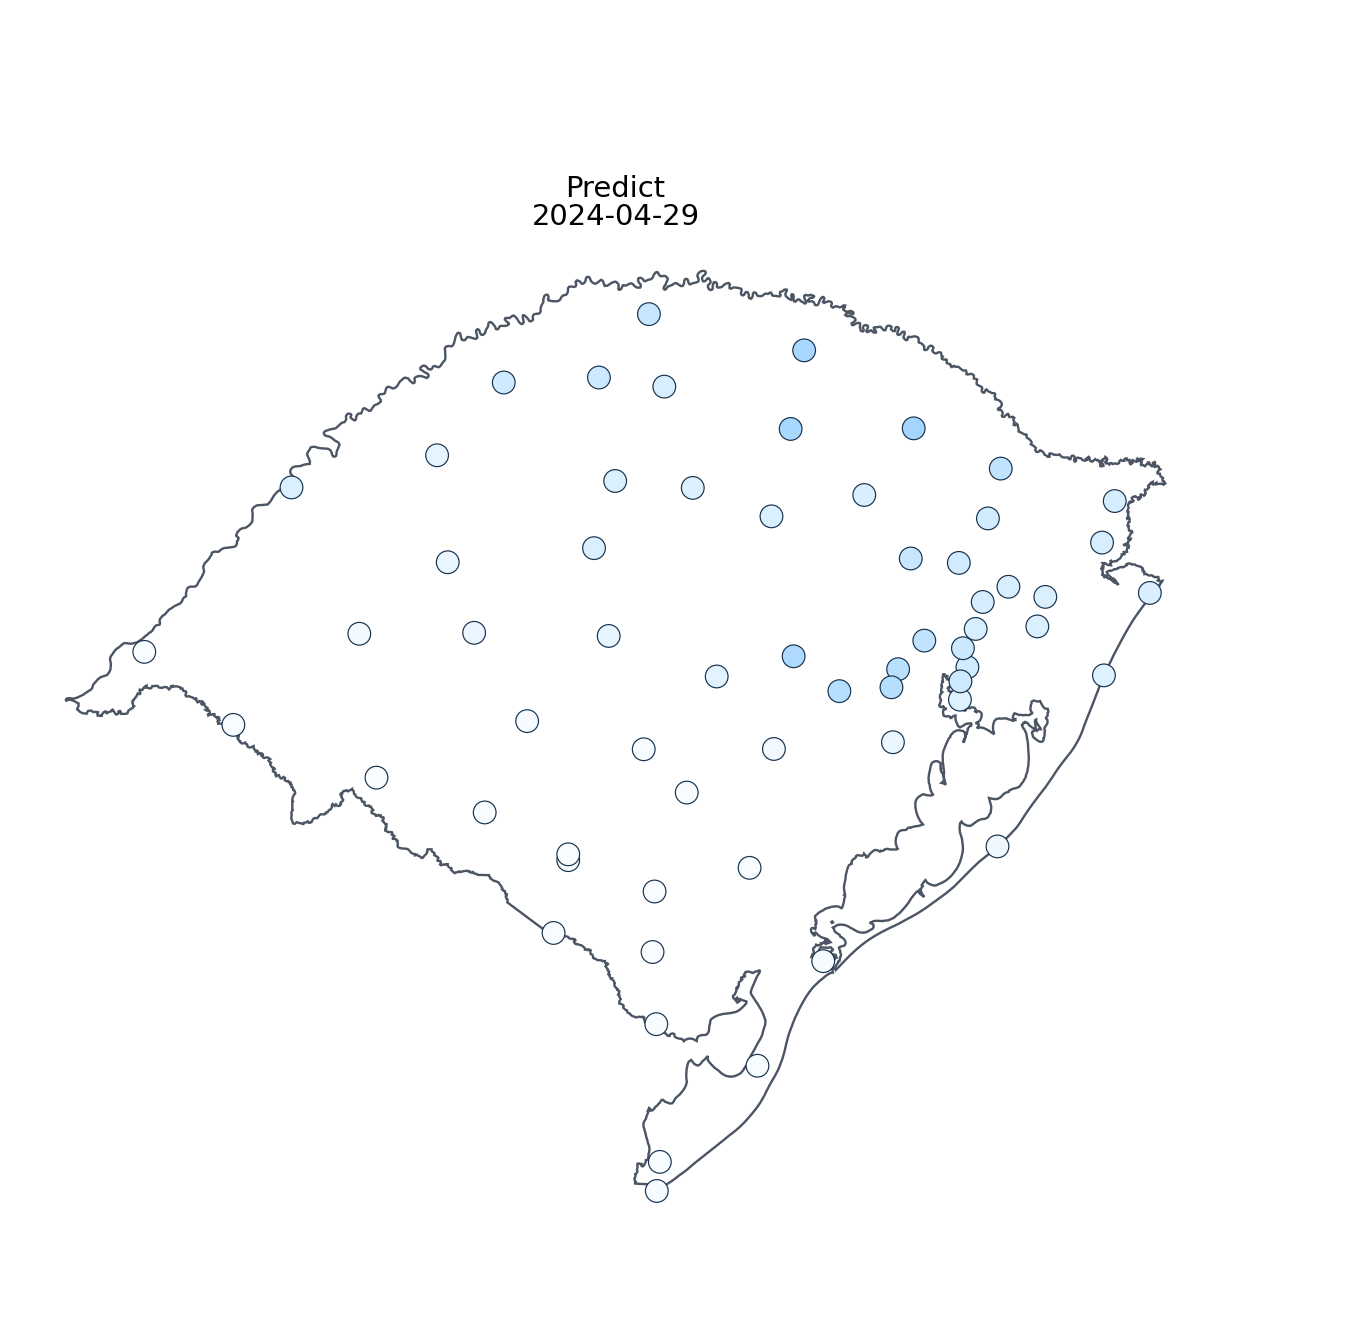
\includegraphics[width=0.48\linewidth]{Predict/frame_010.png}\hfill
    
\includegraphics[width=0.48\linewidth]{Real/frame_010.png}%
  }
  \newframe
  \makebox[\linewidth][c]{%
    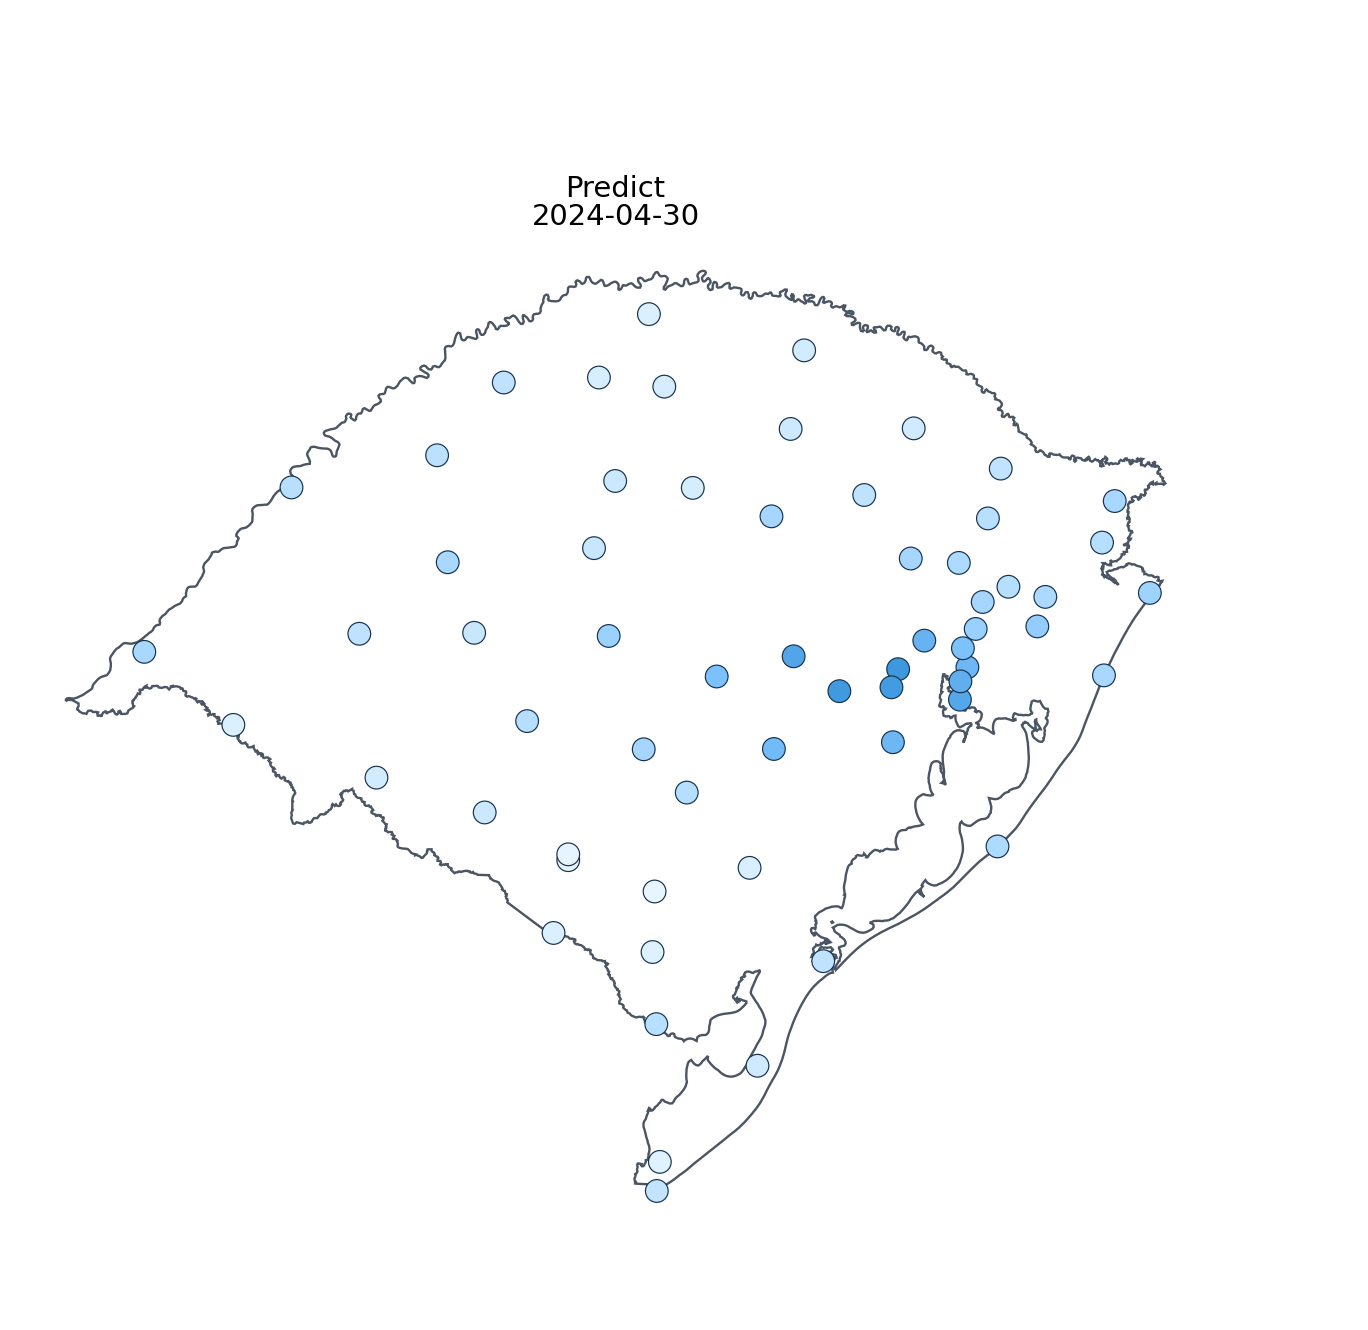
\includegraphics[width=0.48\linewidth]{Predict/frame_011.png}\hfill
    
\includegraphics[width=0.48\linewidth]{Real/frame_011.png}%
  }
  \newframe
  \makebox[\linewidth][c]{%
    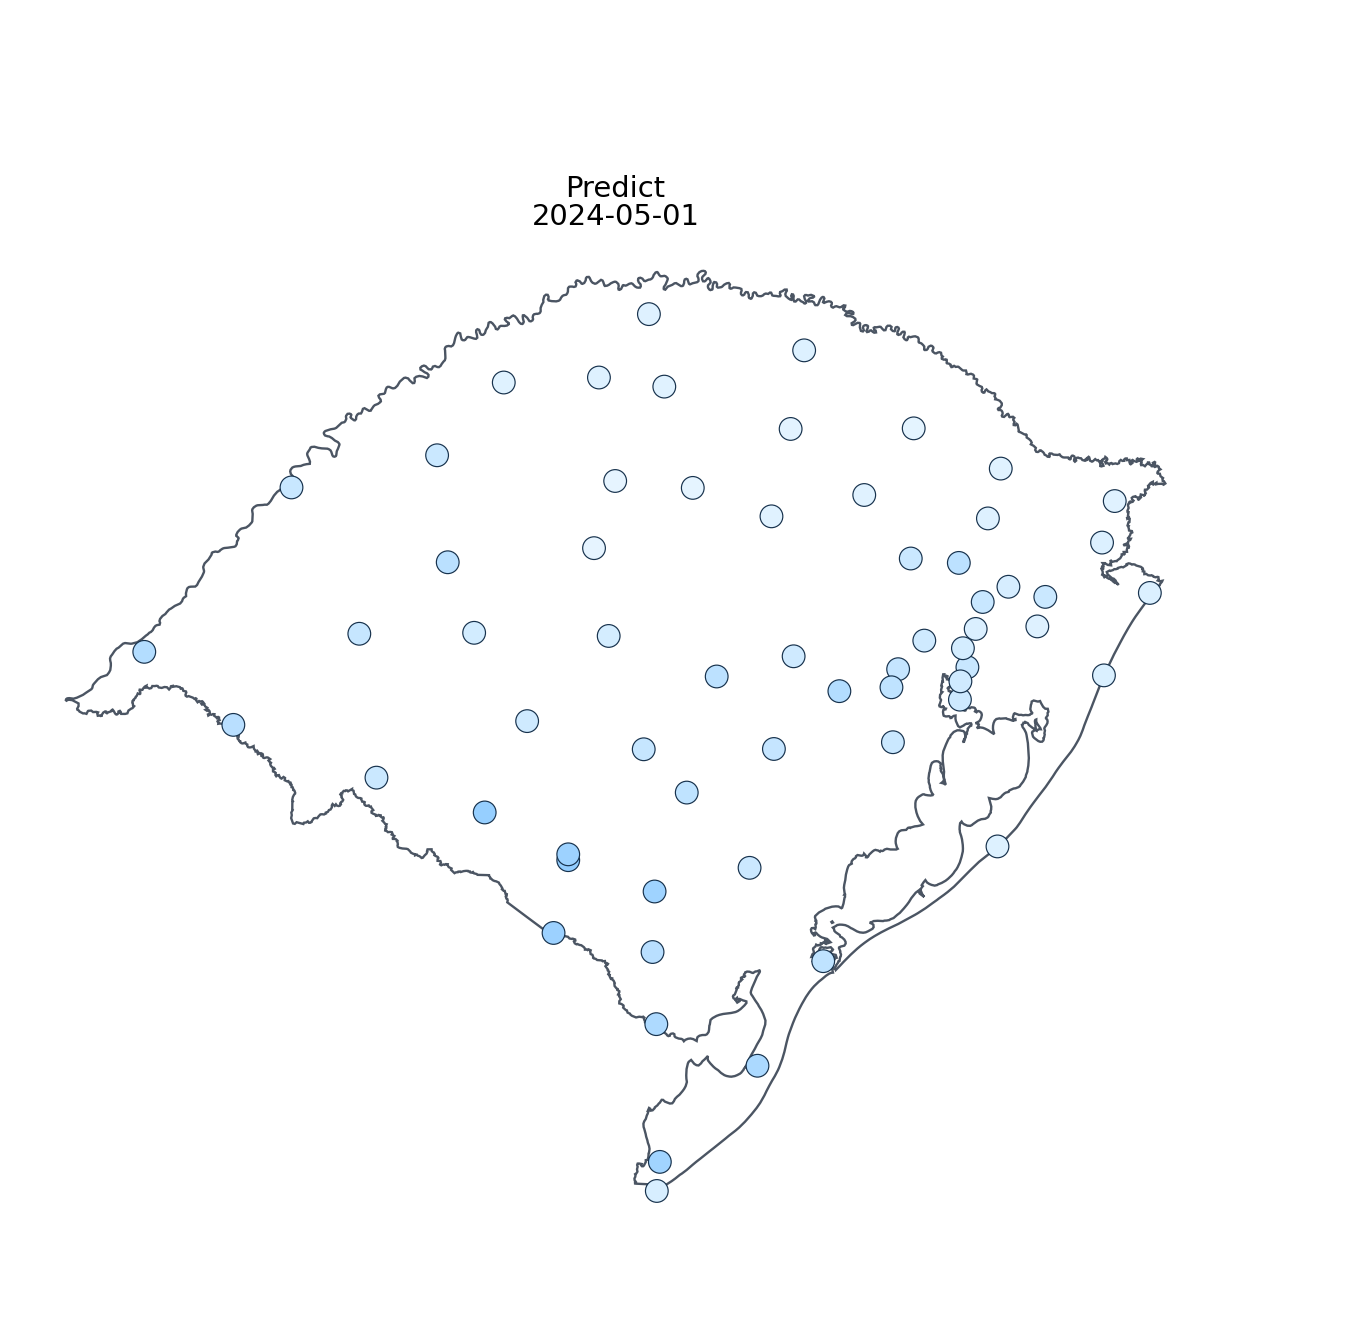
\includegraphics[width=0.48\linewidth]{Predict/frame_012.png}\hfill
    
\includegraphics[width=0.48\linewidth]{Real/frame_012.png}%
  }
  \newframe
  \makebox[\linewidth][c]{%
    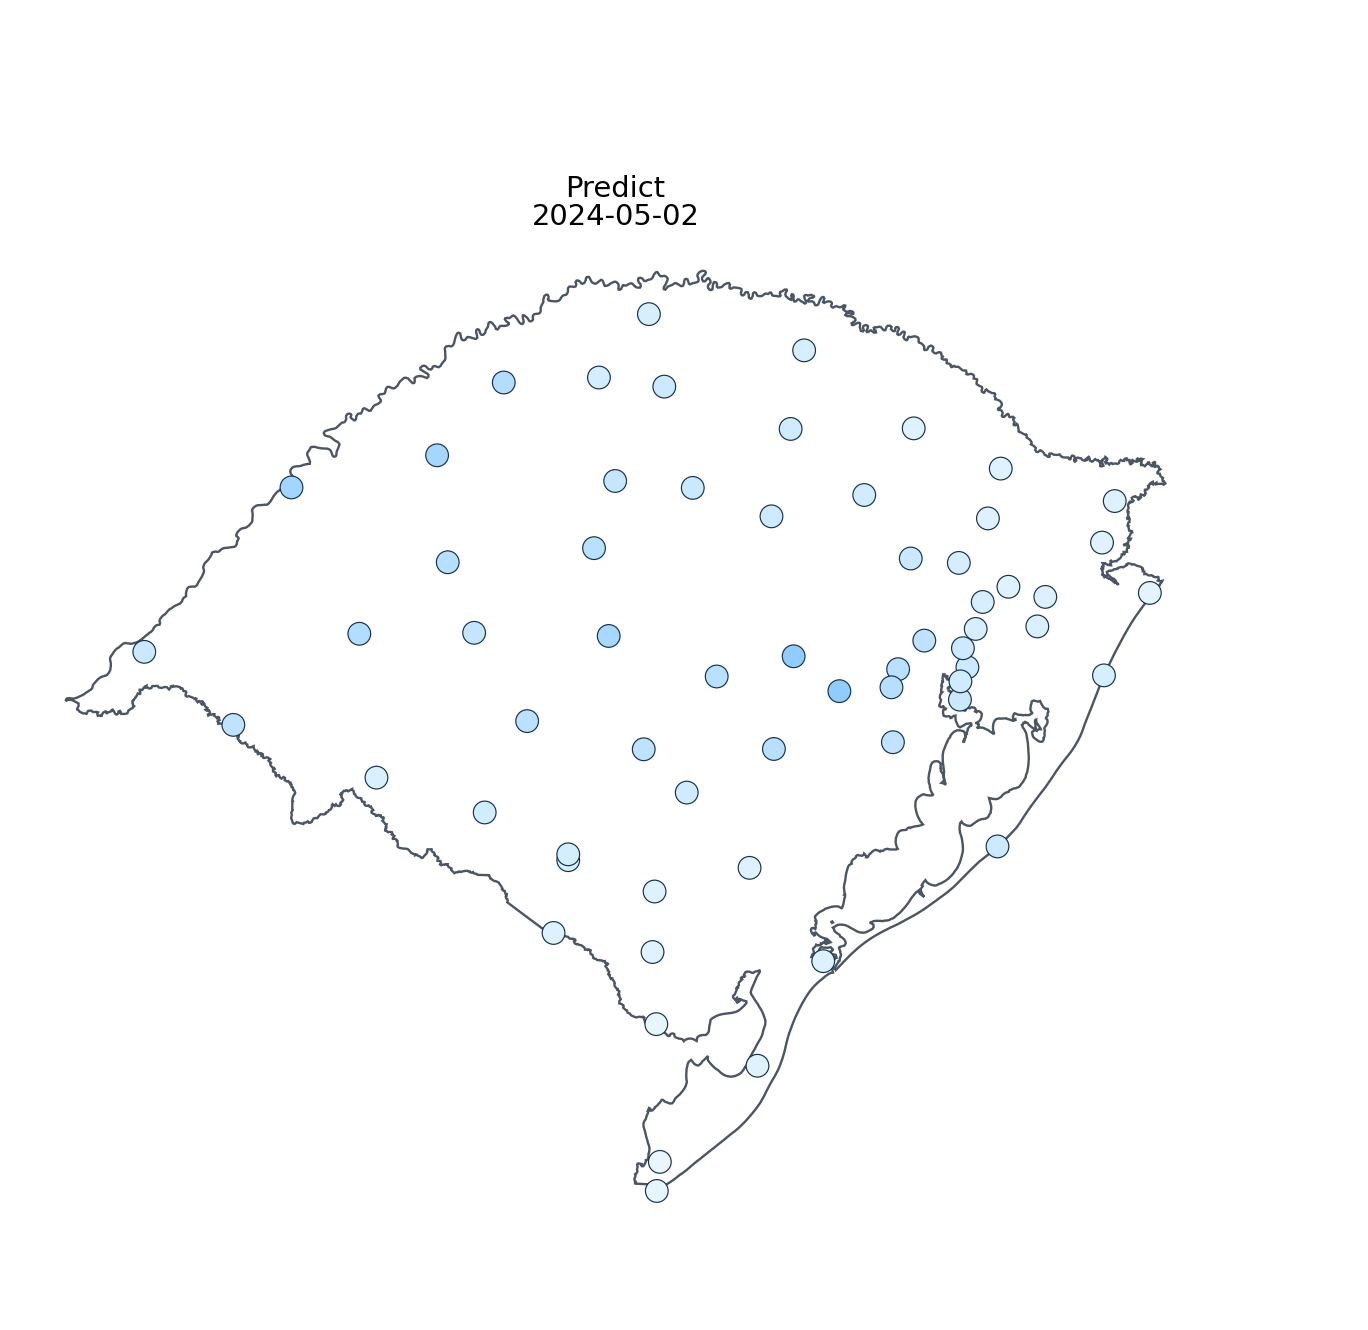
\includegraphics[width=0.48\linewidth]{Predict/frame_013.png}\hfill
    
\includegraphics[width=0.48\linewidth]{Real/frame_013.png}%
  }
  \newframe
  \makebox[\linewidth][c]{%
    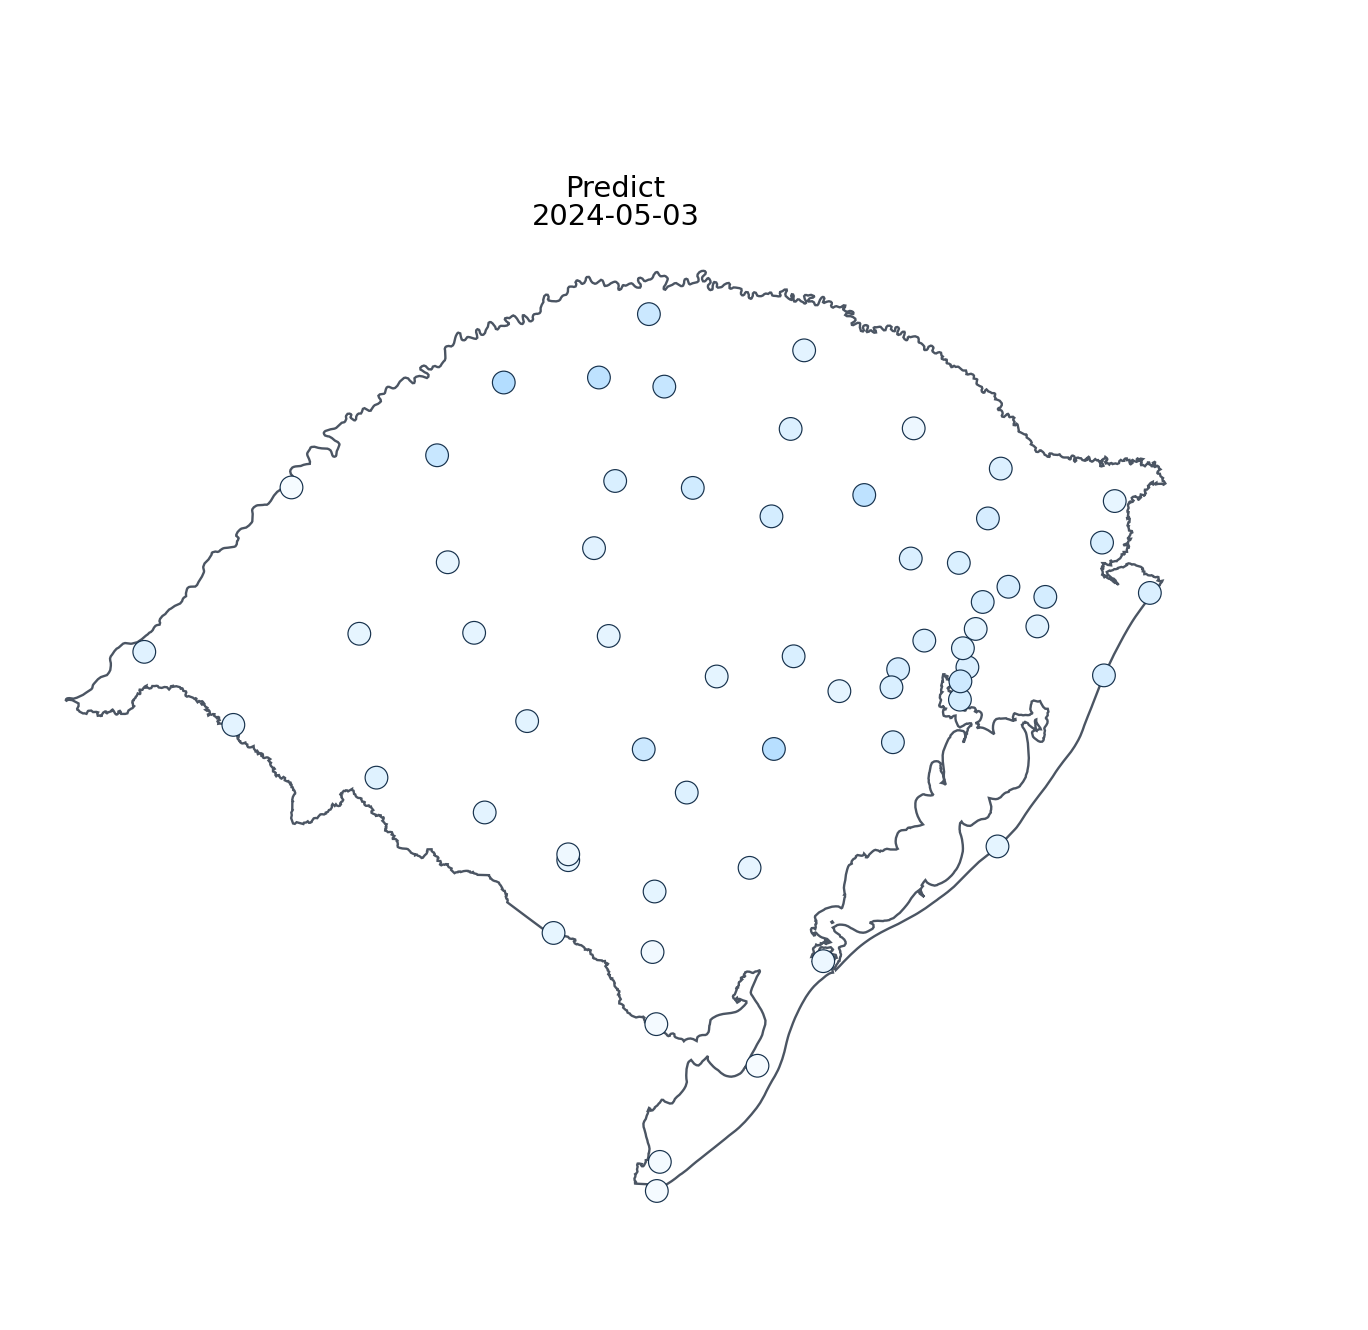
\includegraphics[width=0.48\linewidth]{Predict/frame_014.png}\hfill
    
\includegraphics[width=0.48\linewidth]{Real/frame_014.png}%
  }
  \newframe
  \makebox[\linewidth][c]{%
    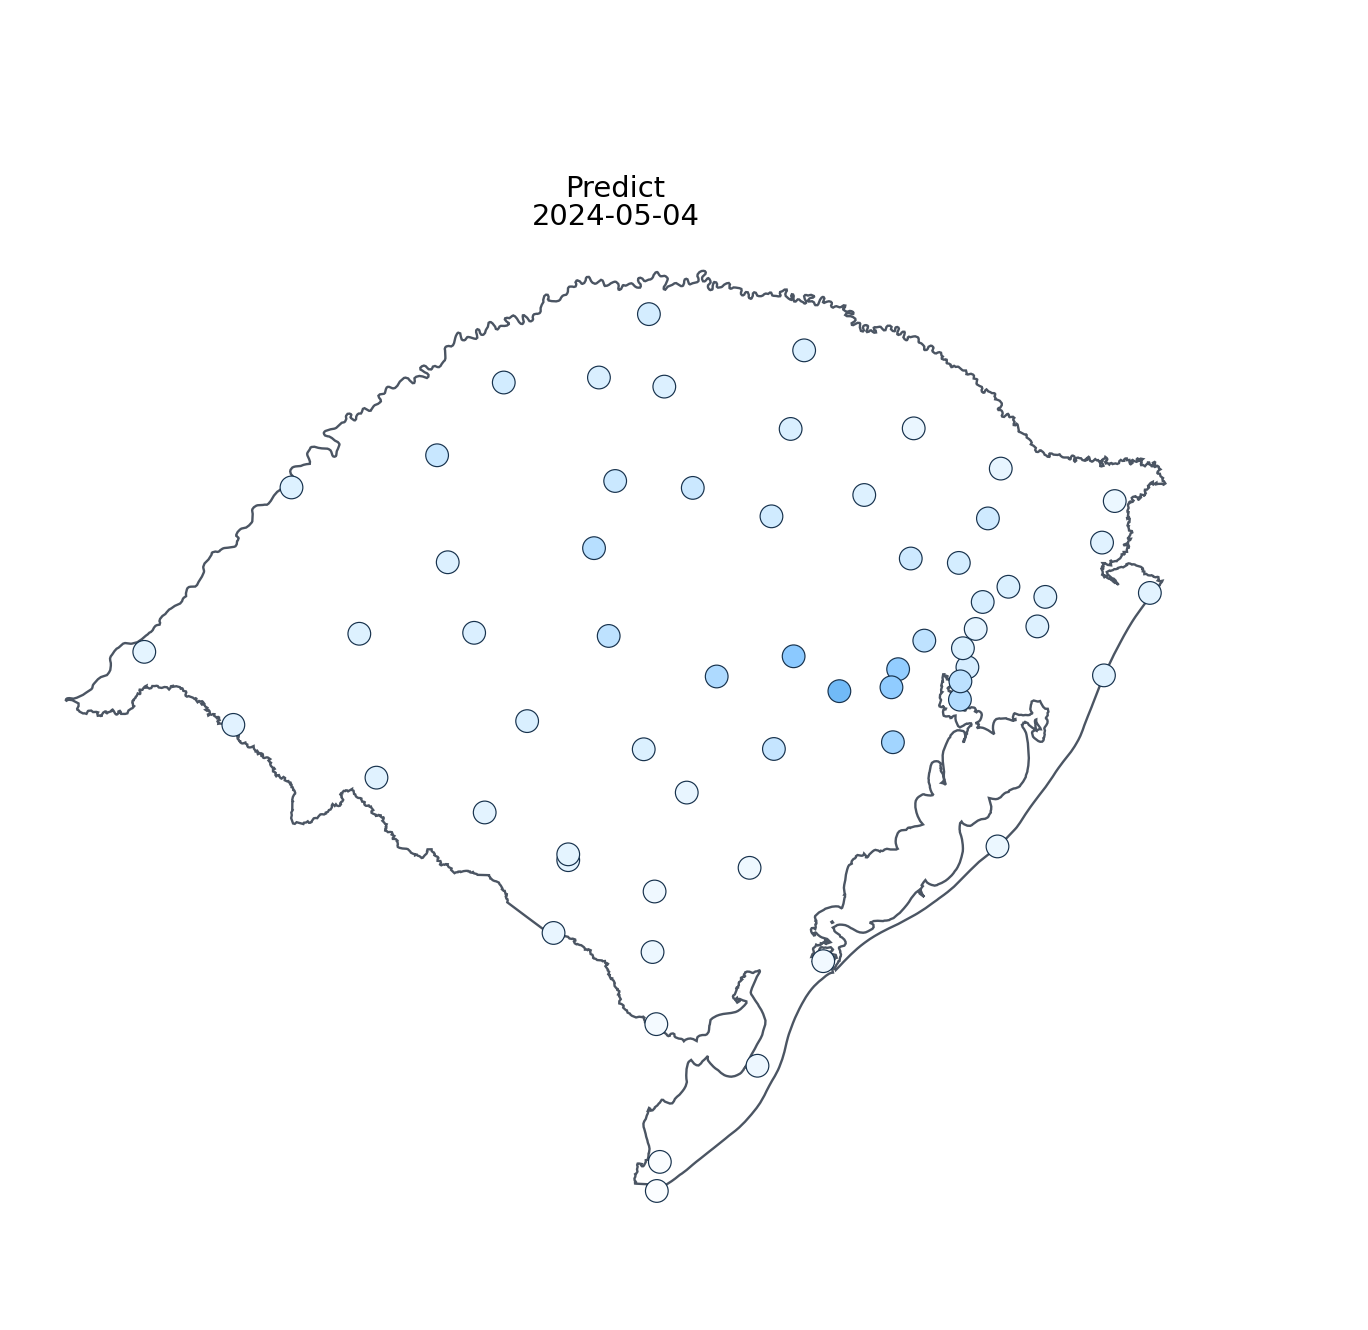
\includegraphics[width=0.48\linewidth]{Predict/frame_015.png}\hfill
    
\includegraphics[width=0.48\linewidth]{Real/frame_015.png}%
  }
  \newframe
  \makebox[\linewidth][c]{%
    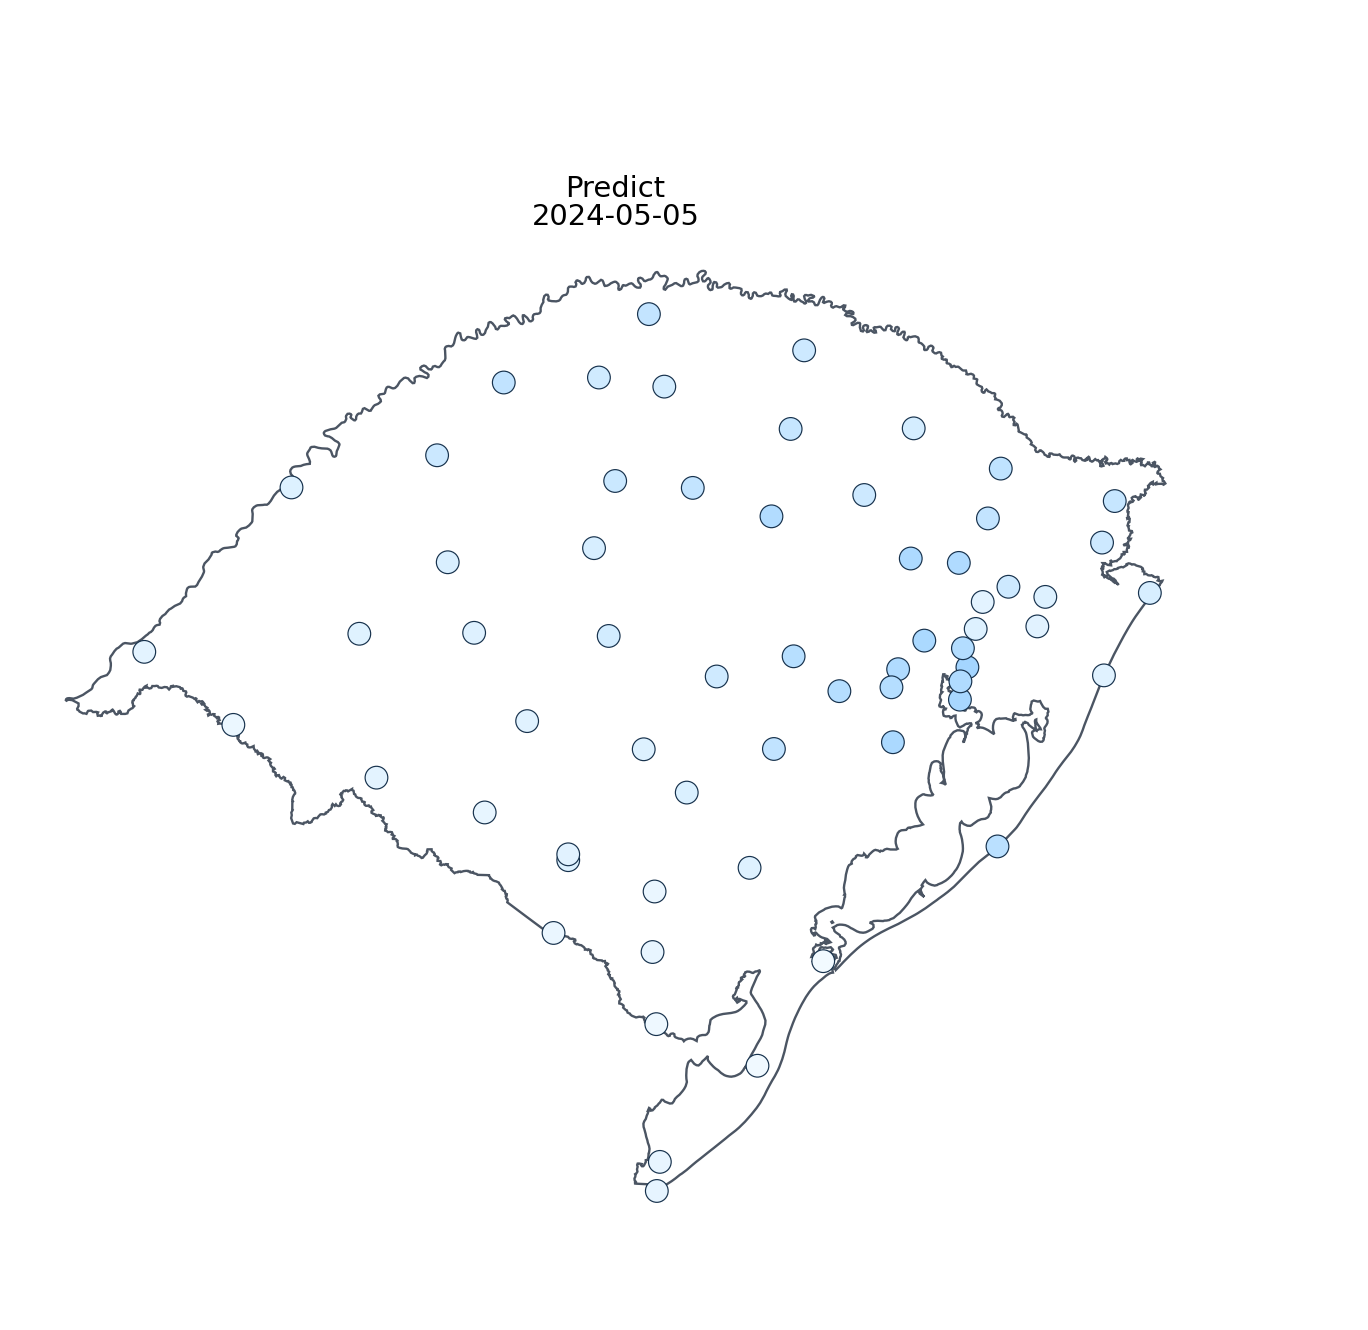
\includegraphics[width=0.48\linewidth]{Predict/frame_016.png}\hfill
    
\includegraphics[width=0.48\linewidth]{Real/frame_016.png}%
  }
  \newframe
  \makebox[\linewidth][c]{%
    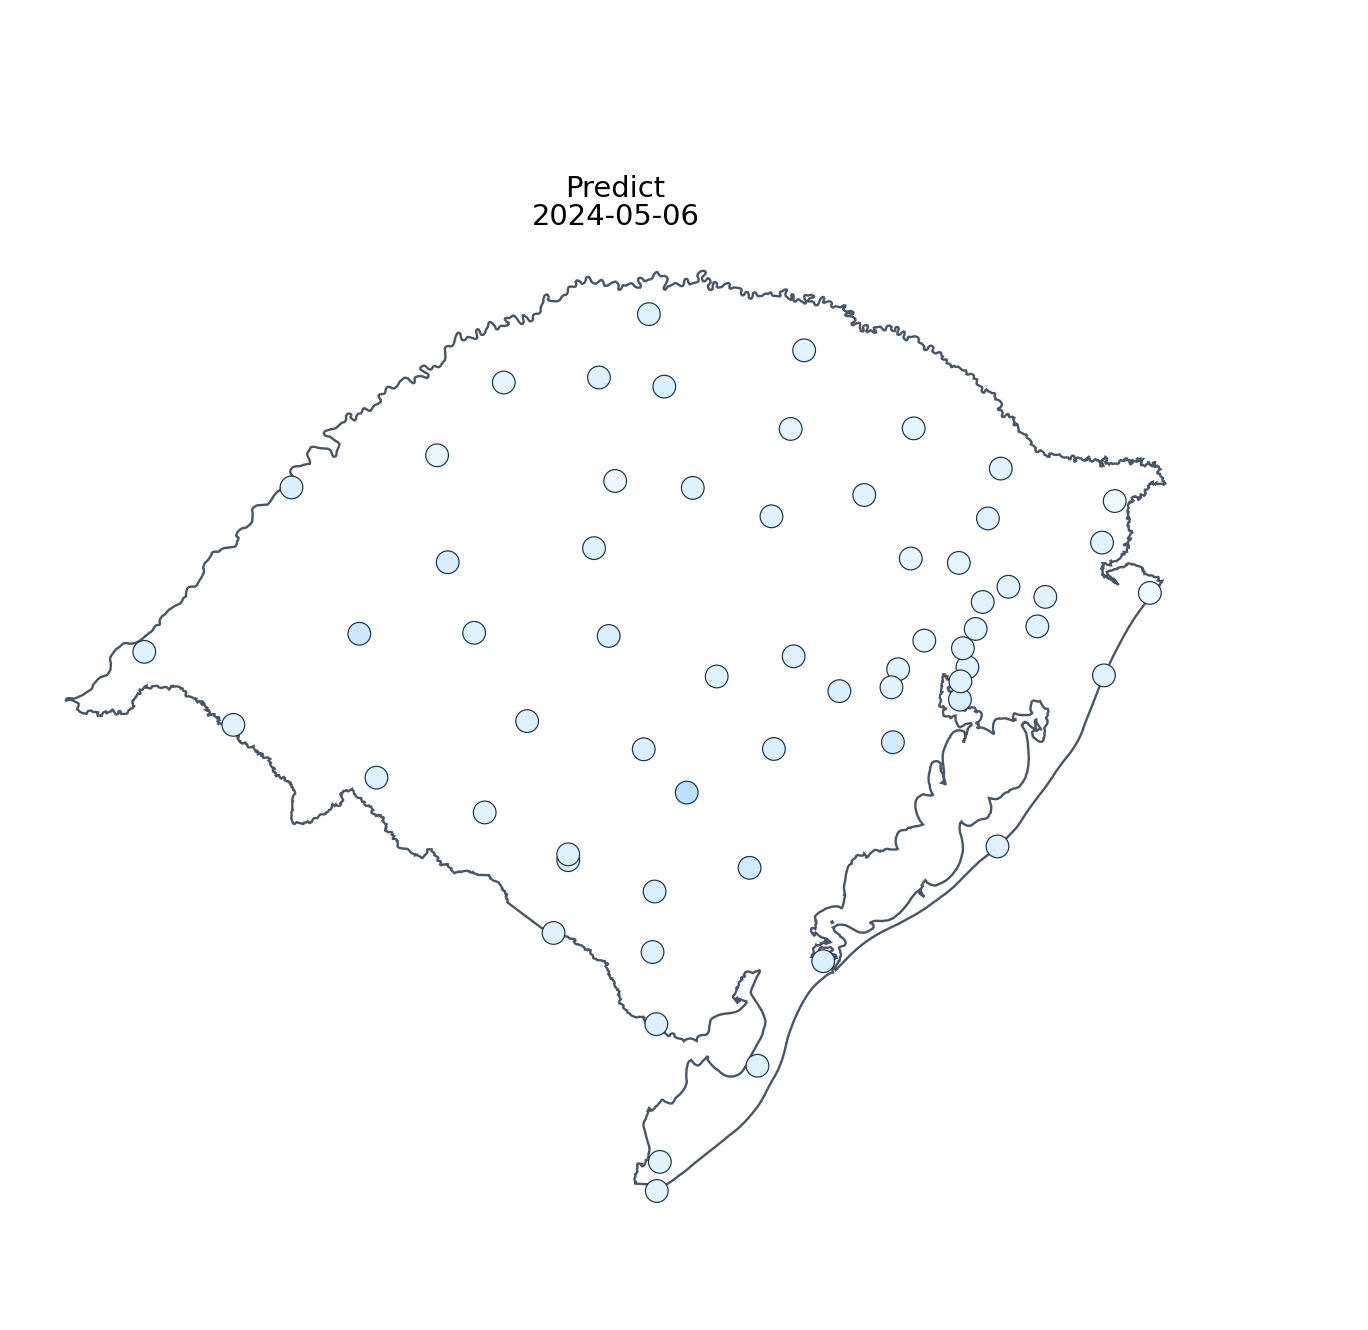
\includegraphics[width=0.48\linewidth]{Predict/frame_017.png}\hfill
    
\includegraphics[width=0.48\linewidth]{Real/frame_017.png}%
  }
  \newframe
  \makebox[\linewidth][c]{%
    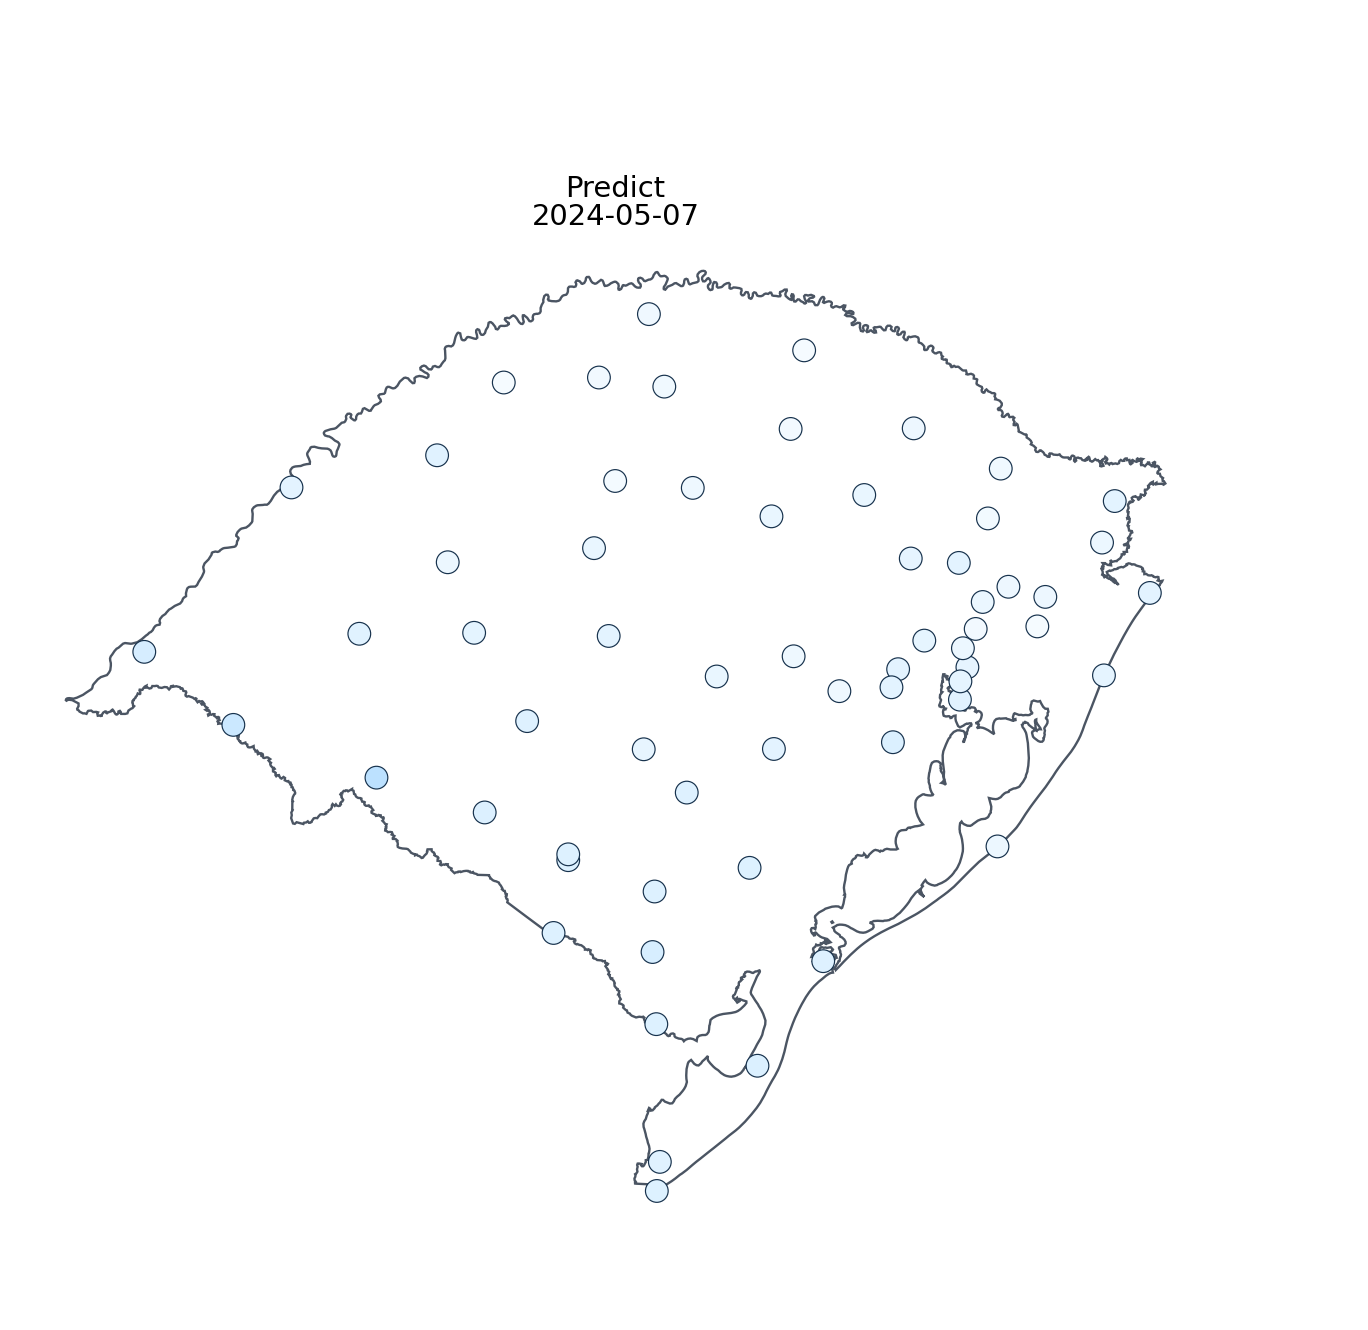
\includegraphics[width=0.48\linewidth]{Predict/frame_018.png}\hfill
    
\includegraphics[width=0.48\linewidth]{Real/frame_018.png}%
  }
  \newframe
  \makebox[\linewidth][c]{%
    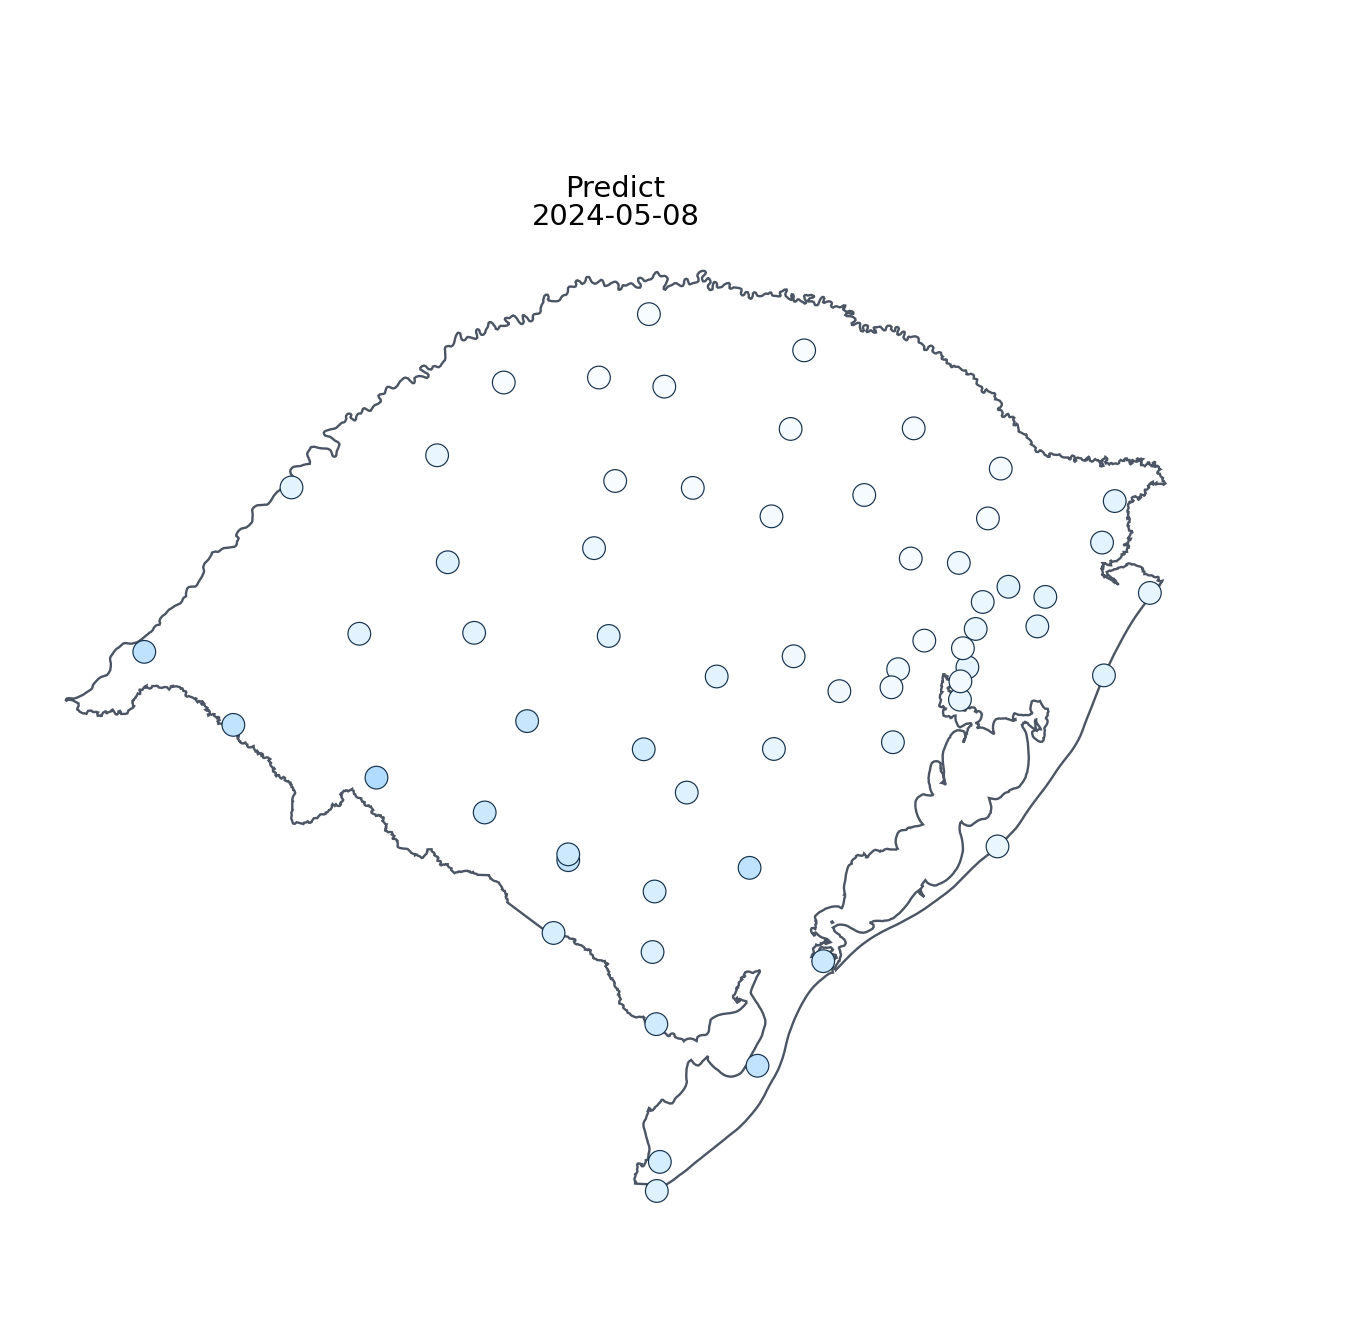
\includegraphics[width=0.48\linewidth]{Predict/frame_019.png}\hfill
    
\includegraphics[width=0.48\linewidth]{Real/frame_019.png}%
  }
  \newframe
  \makebox[\linewidth][c]{%
    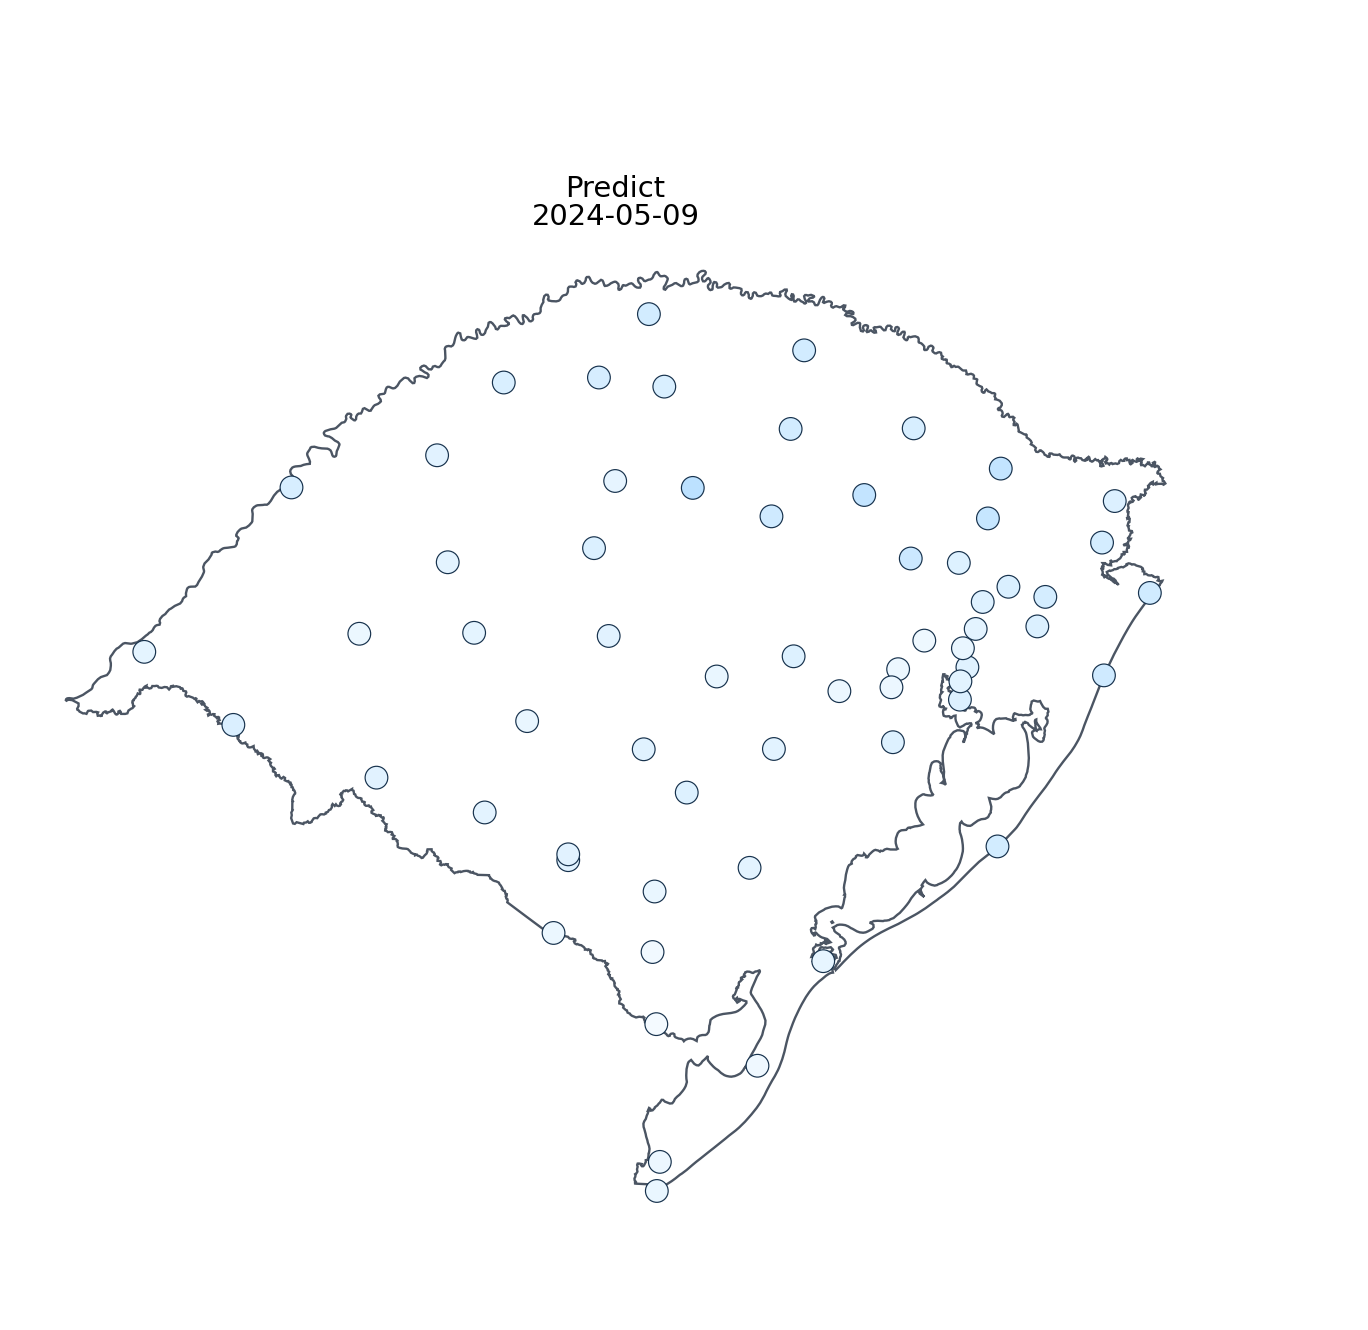
\includegraphics[width=0.48\linewidth]{Predict/frame_020.png}\hfill
    
\includegraphics[width=0.48\linewidth]{Real/frame_020.png}%
  }
  \newframe
  \makebox[\linewidth][c]{%
    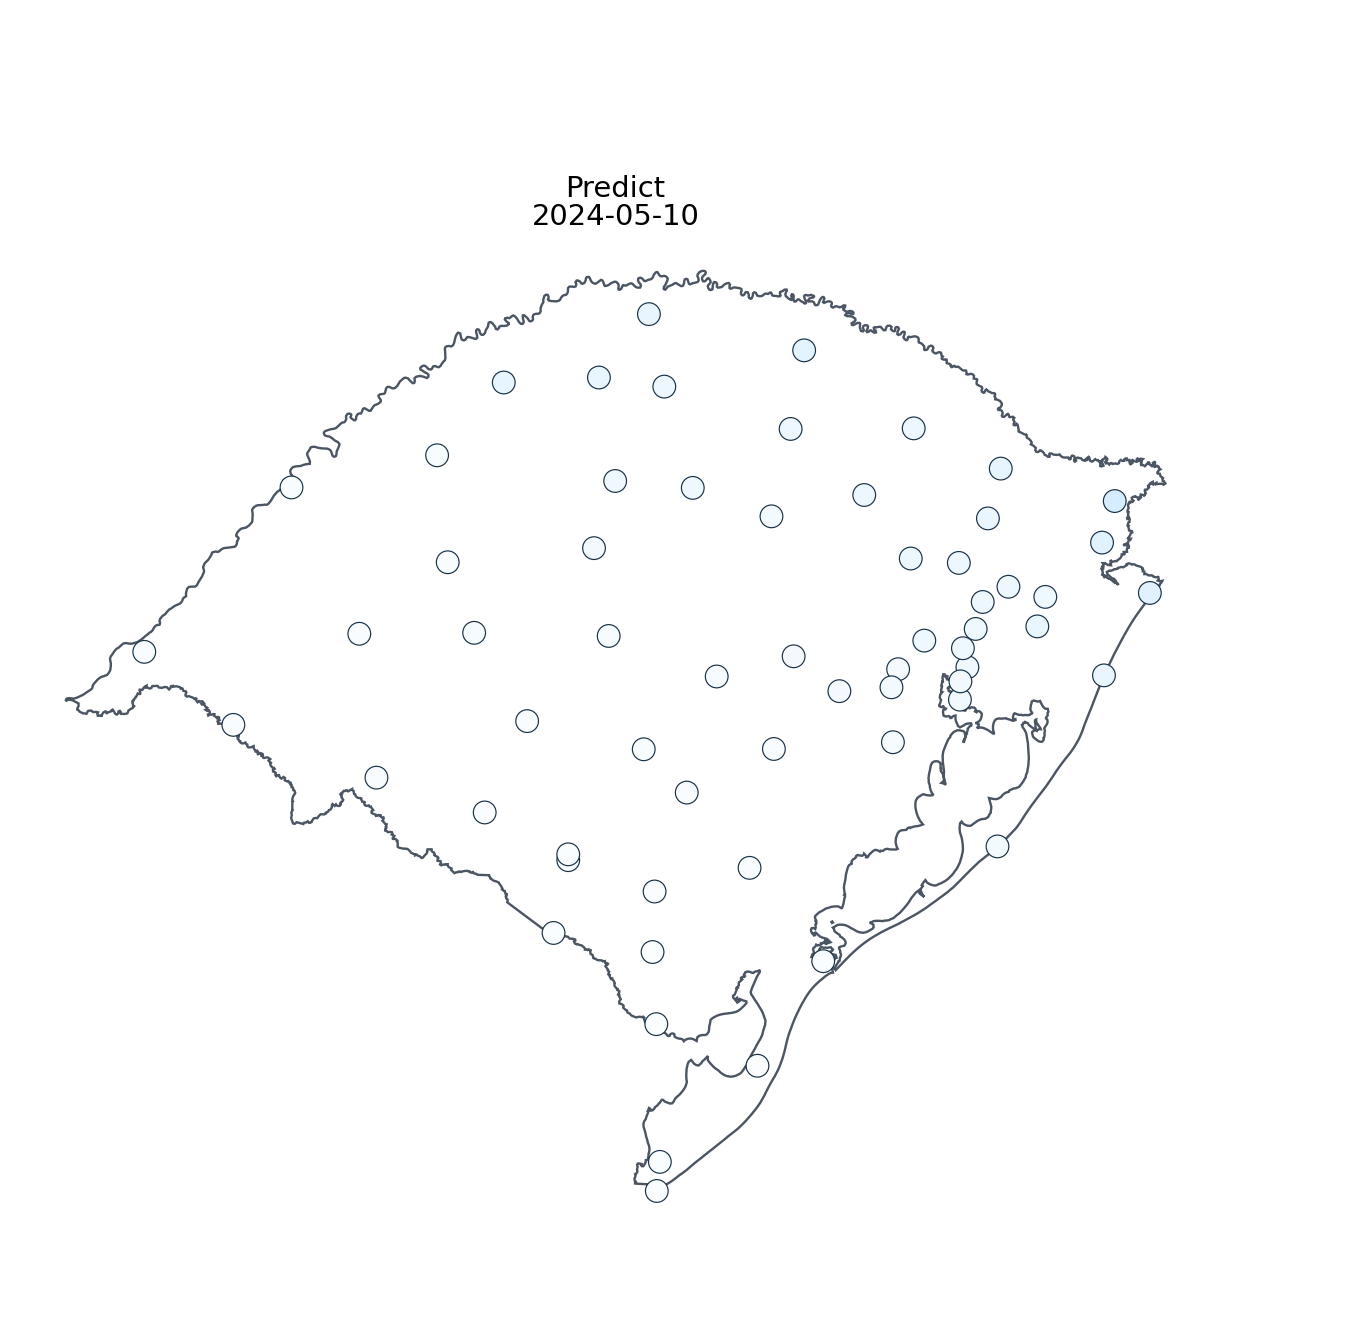
\includegraphics[width=0.48\linewidth]{Predict/frame_021.png}\hfill
    
\includegraphics[width=0.48\linewidth]{Real/frame_021.png}%
  }
  \newframe
  \makebox[\linewidth][c]{%
    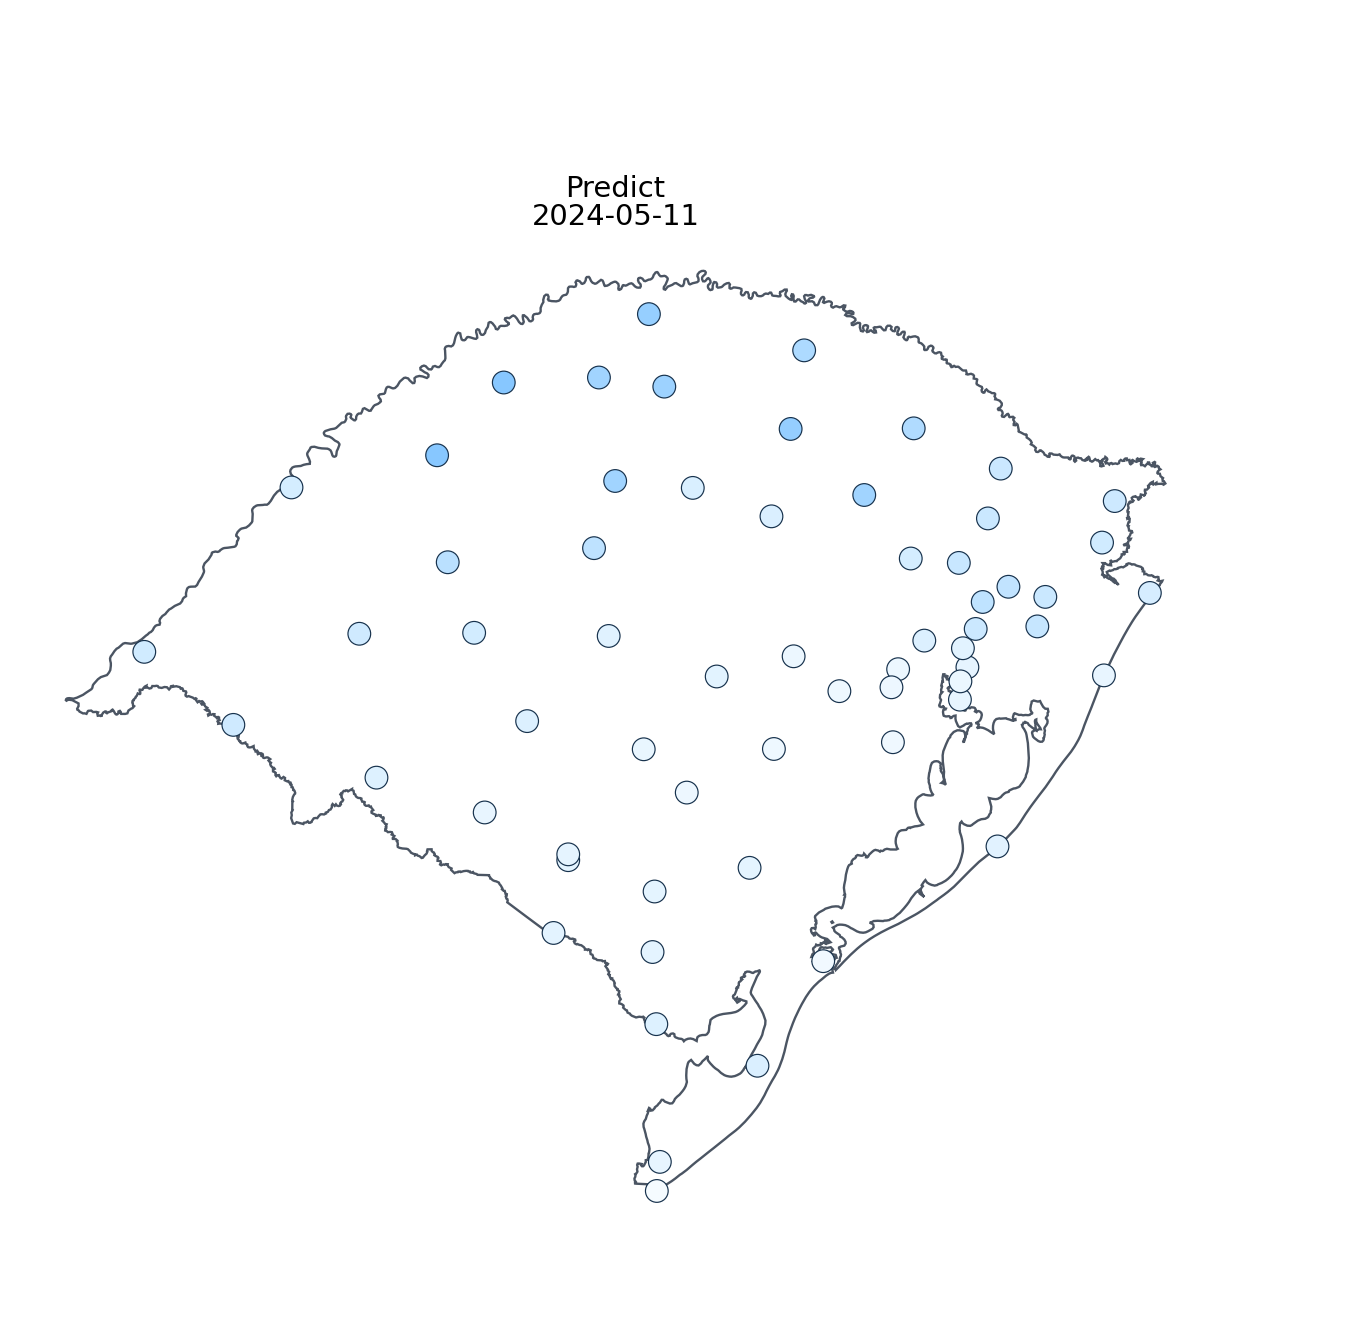
\includegraphics[width=0.48\linewidth]{Predict/frame_022.png}\hfill
    
\includegraphics[width=0.48\linewidth]{Real/frame_022.png}%
  }
  \newframe
  \makebox[\linewidth][c]{%
    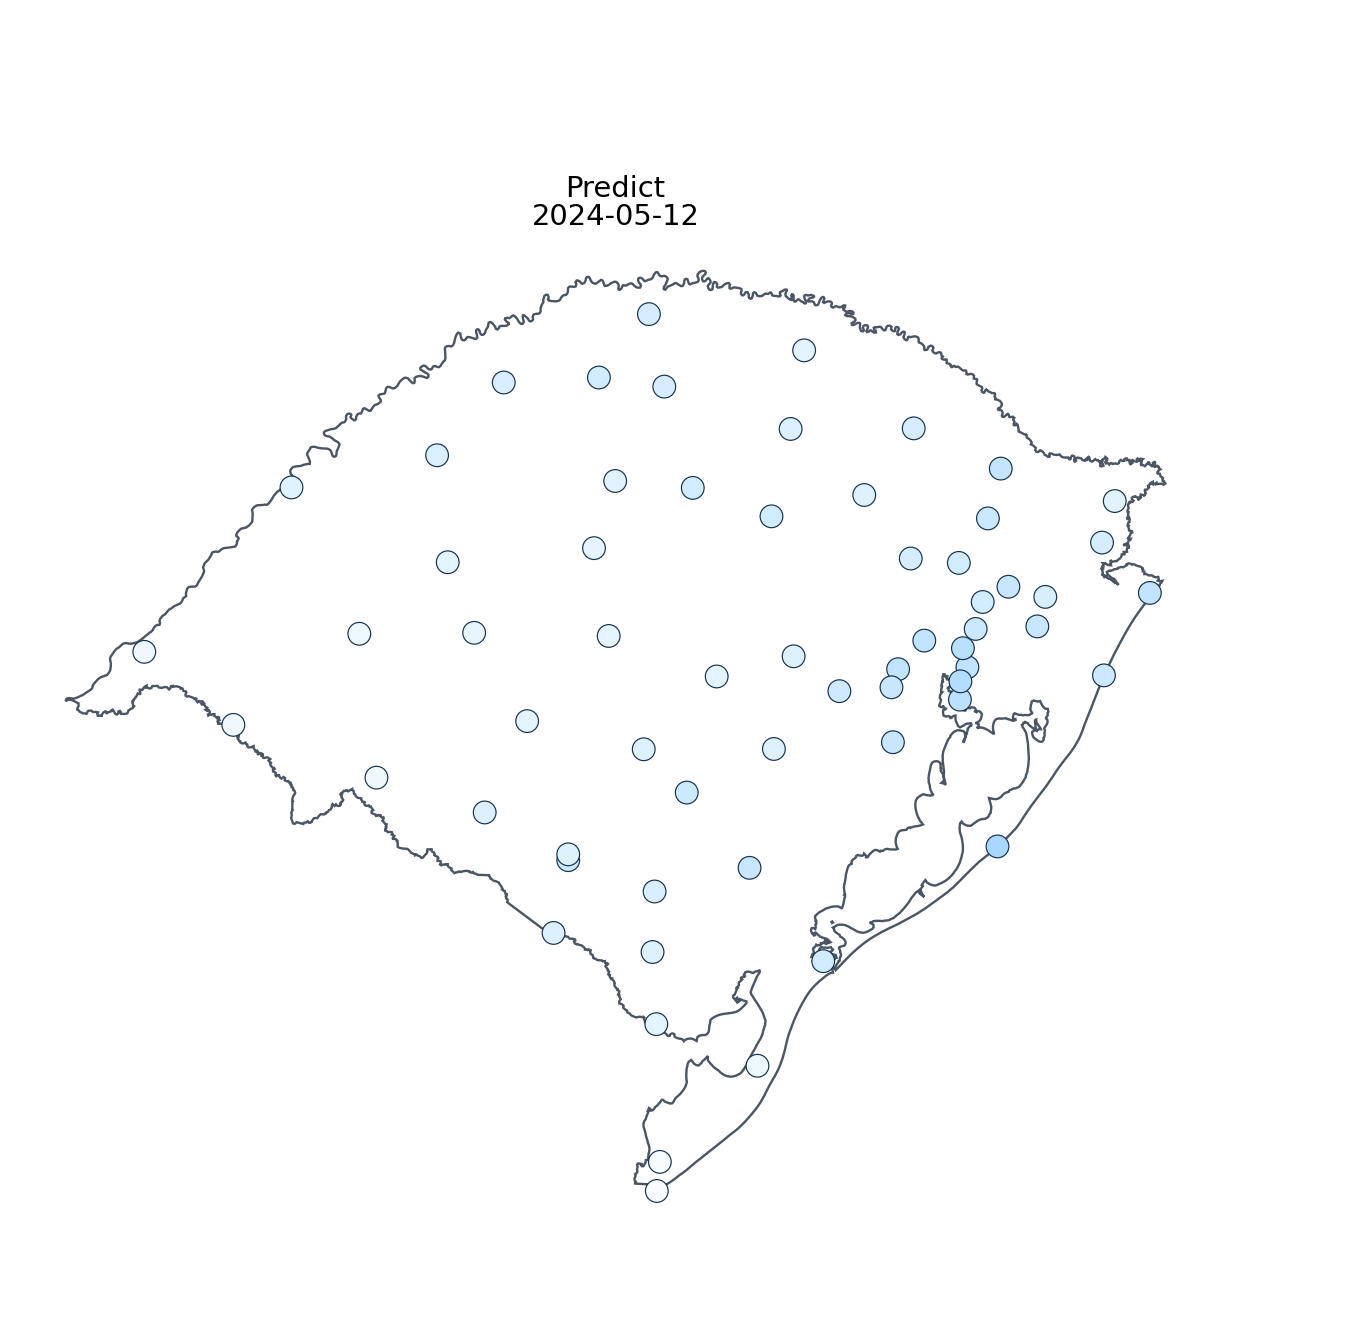
\includegraphics[width=0.48\linewidth]{Predict/frame_023.png}\hfill
    
\includegraphics[width=0.48\linewidth]{Real/frame_023.png}%
  }
  \newframe
  \makebox[\linewidth][c]{%
    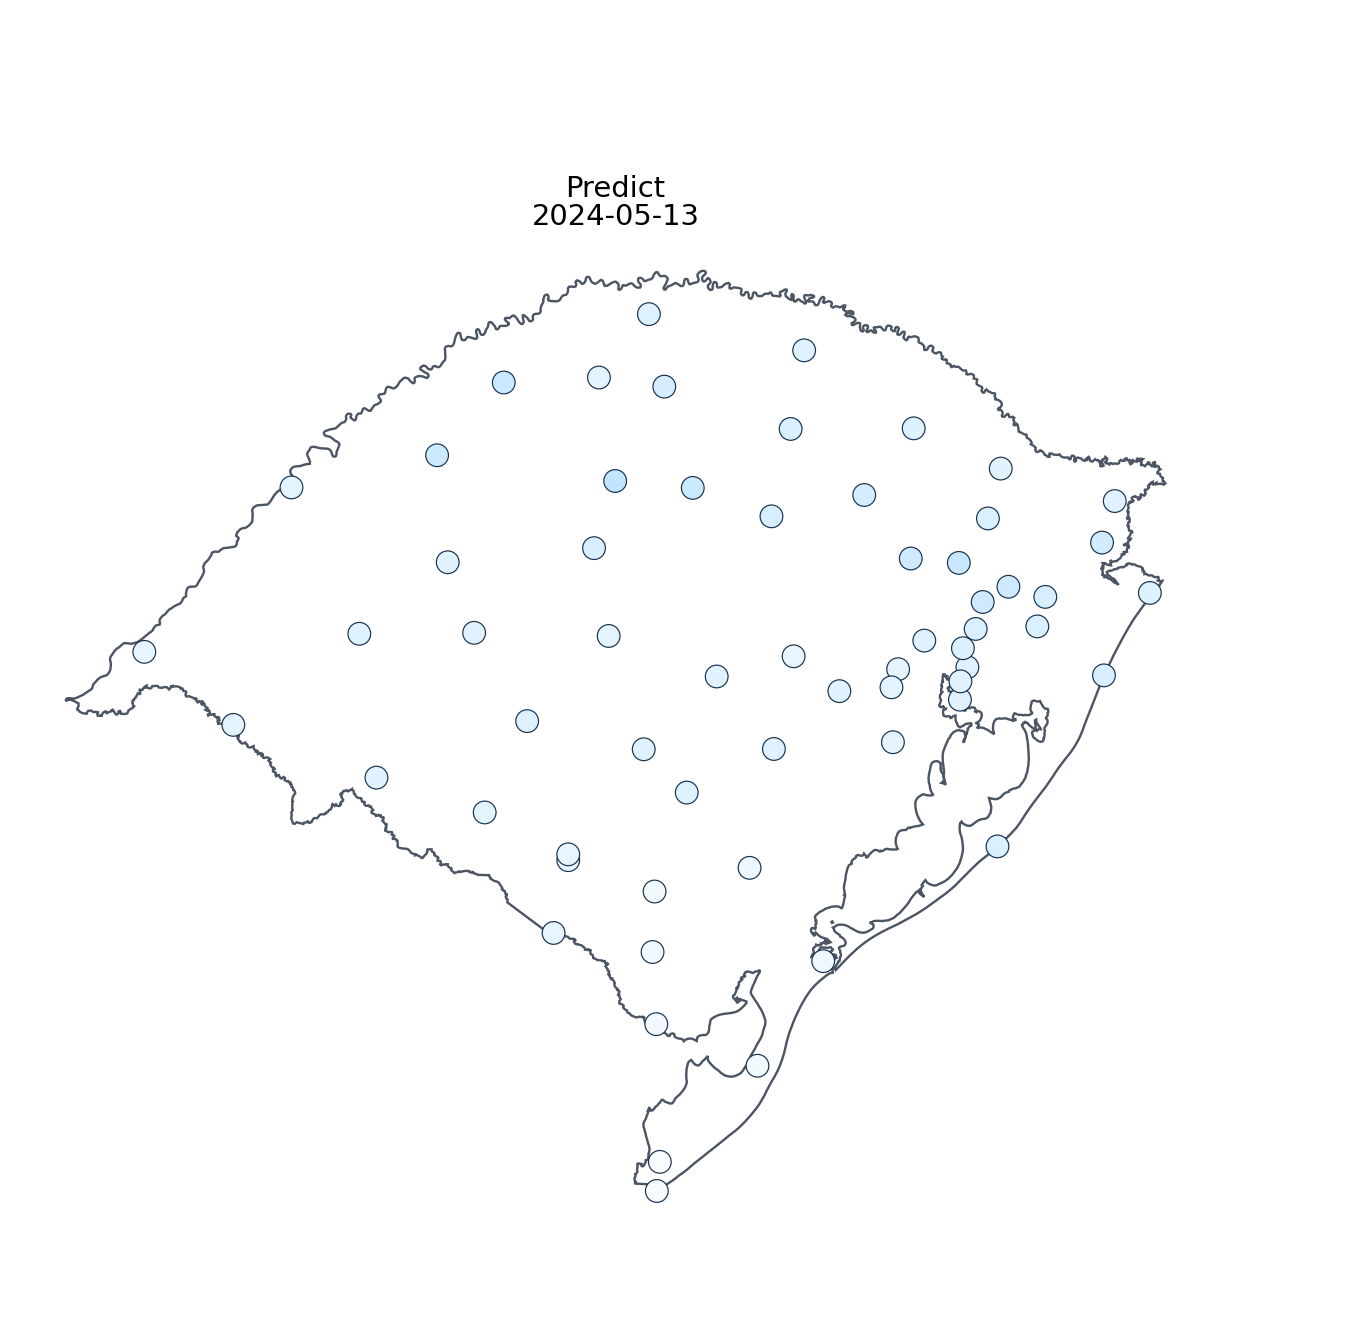
\includegraphics[width=0.48\linewidth]{Predict/frame_024.png}\hfill
    
\includegraphics[width=0.48\linewidth]{Real/frame_024.png}%
  }
  \newframe
  \makebox[\linewidth][c]{%
    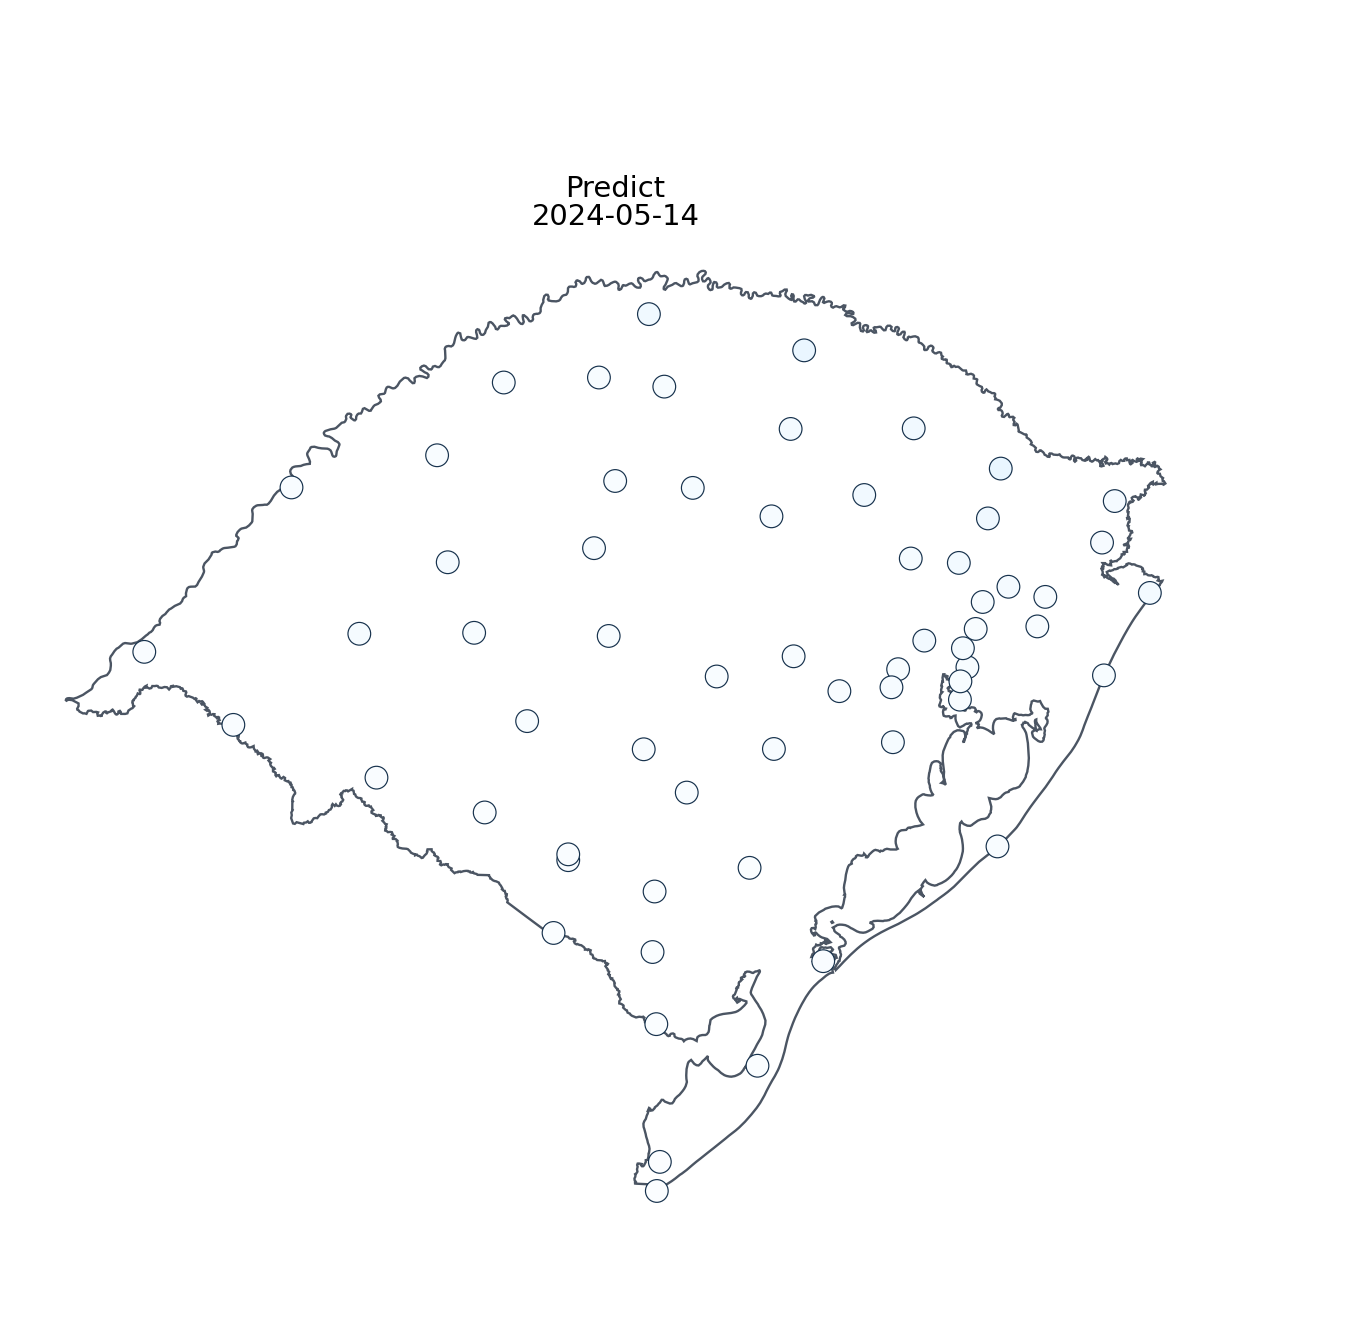
\includegraphics[width=0.48\linewidth]{Predict/frame_025.png}\hfill
    
\includegraphics[width=0.48\linewidth]{Real/frame_025.png}%
  }
  \newframe
  \makebox[\linewidth][c]{%
    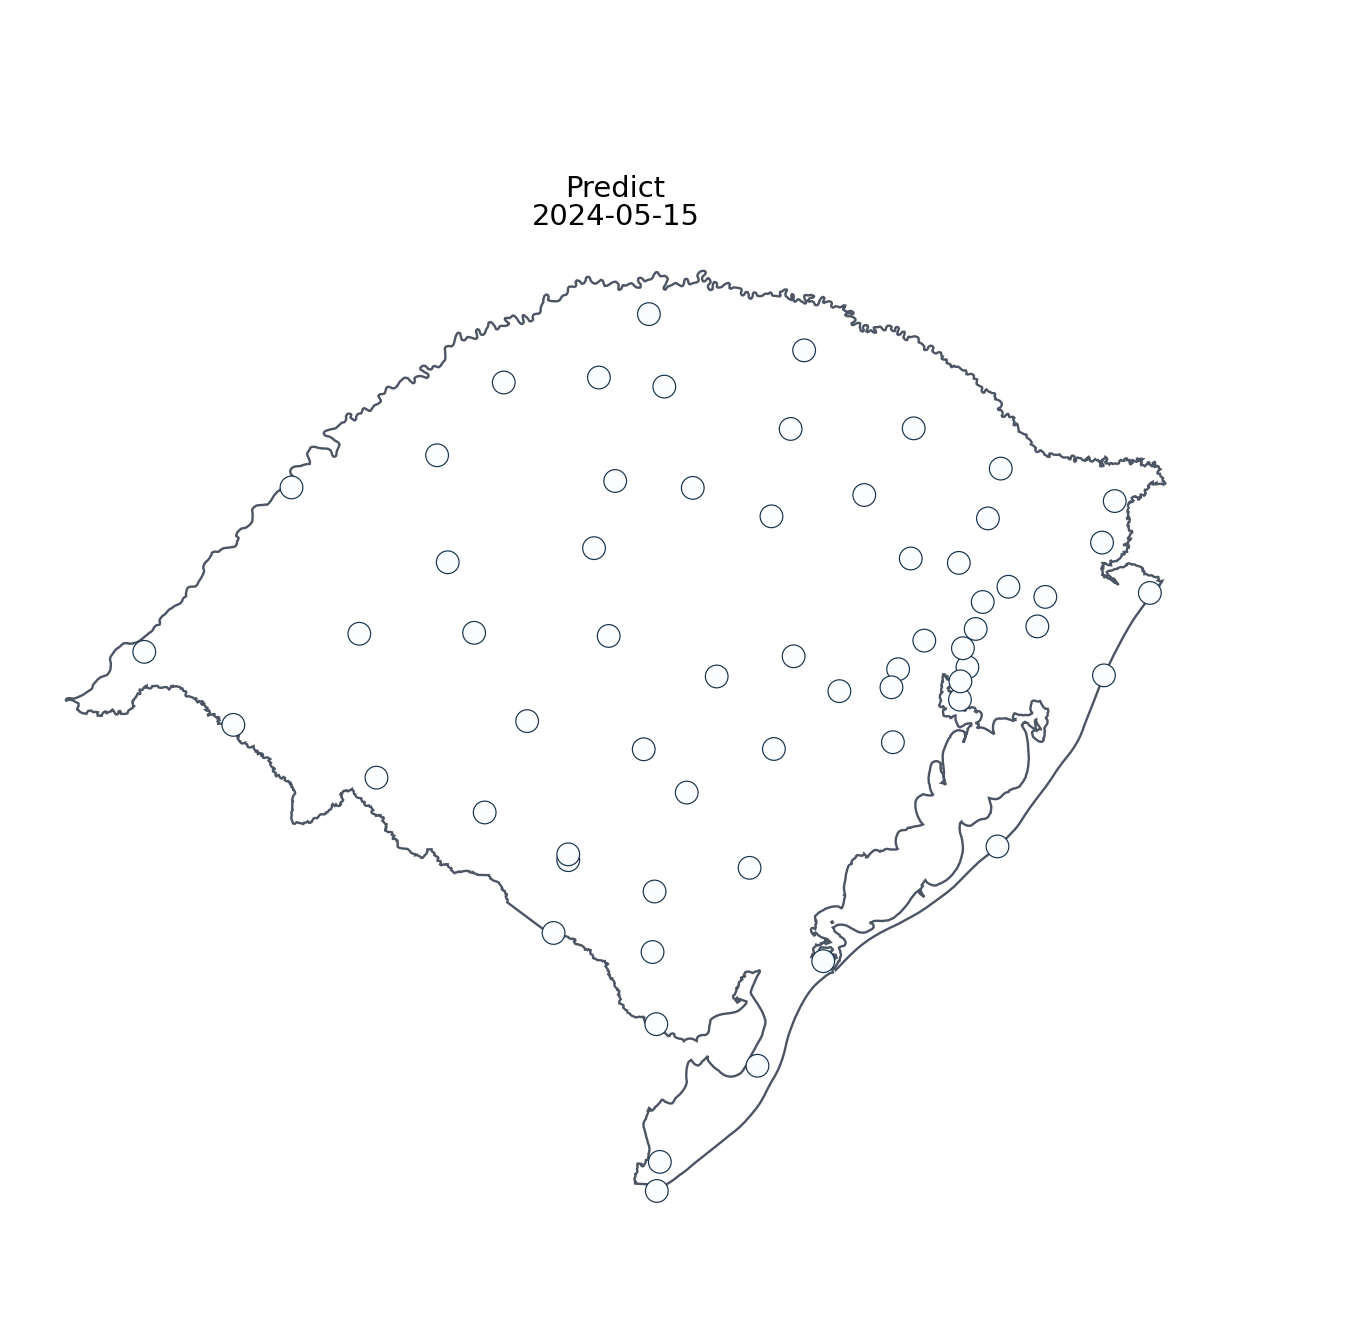
\includegraphics[width=0.48\linewidth]{Predict/frame_026.png}\hfill
    
\includegraphics[width=0.48\linewidth]{Real/frame_026.png}%
  }
  \newframe
  \makebox[\linewidth][c]{%
    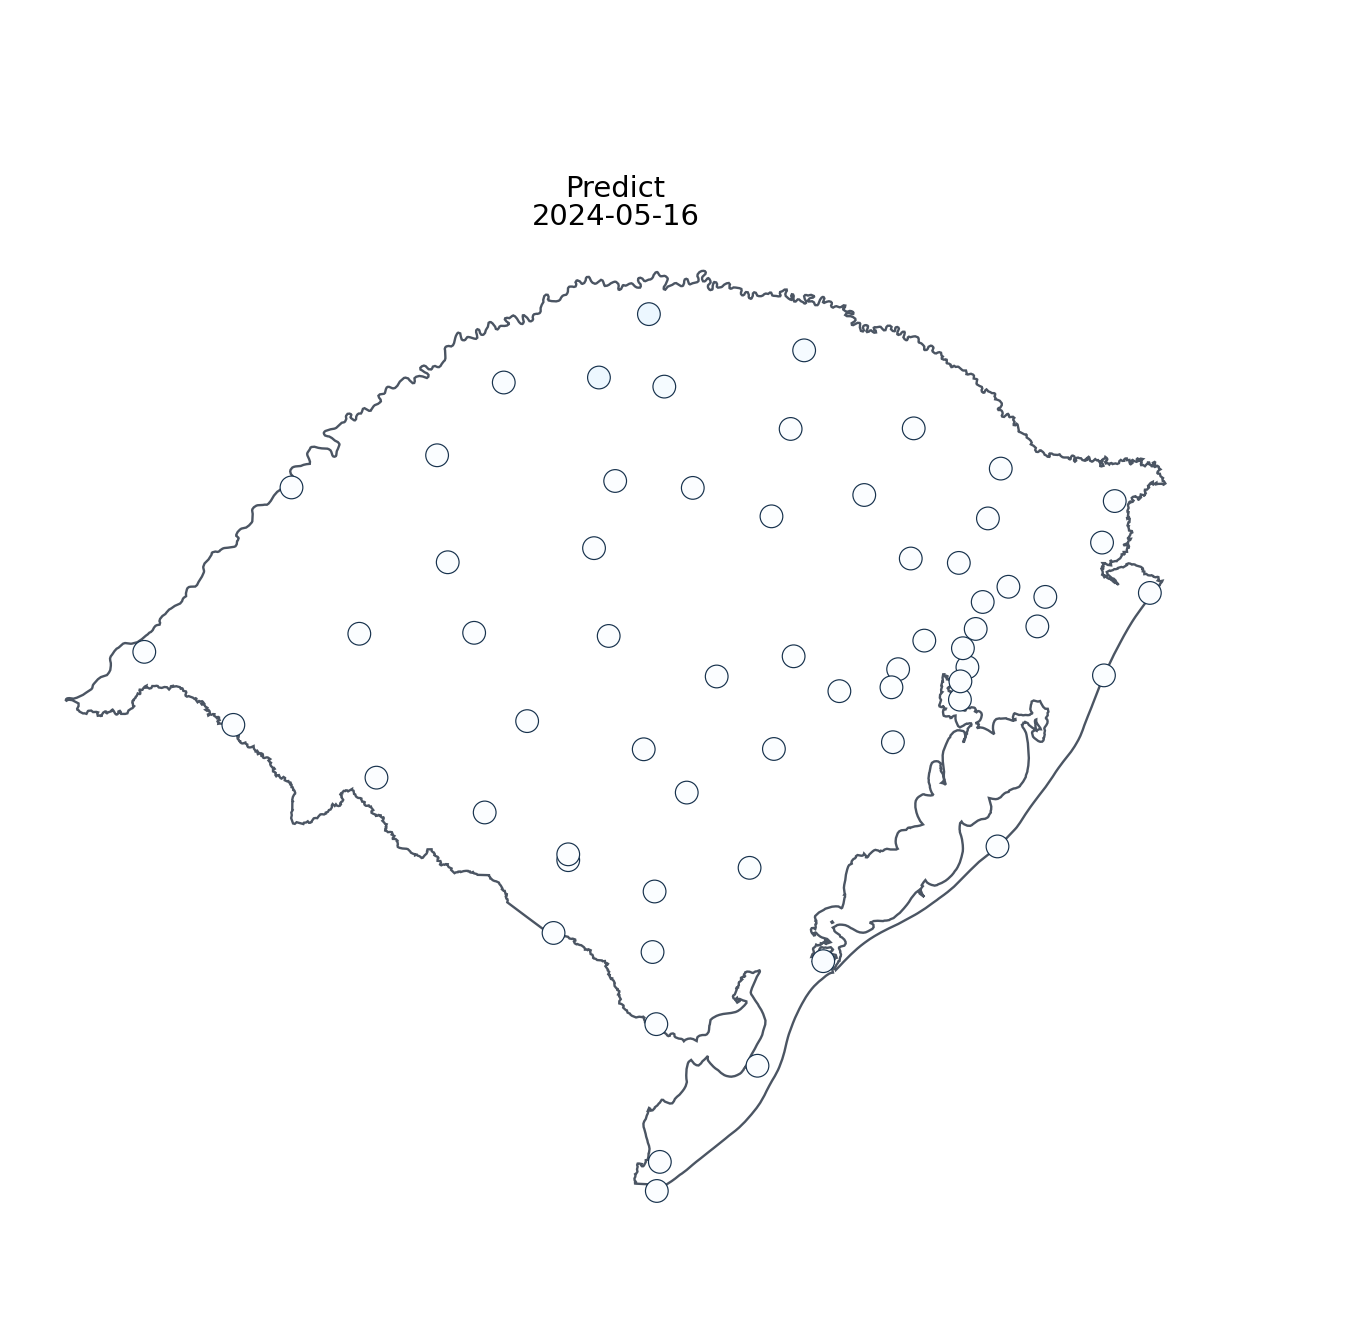
\includegraphics[width=0.48\linewidth]{Predict/frame_027.png}\hfill
    
\includegraphics[width=0.48\linewidth]{Real/frame_027.png}%
  }
  \newframe
  \makebox[\linewidth][c]{%
    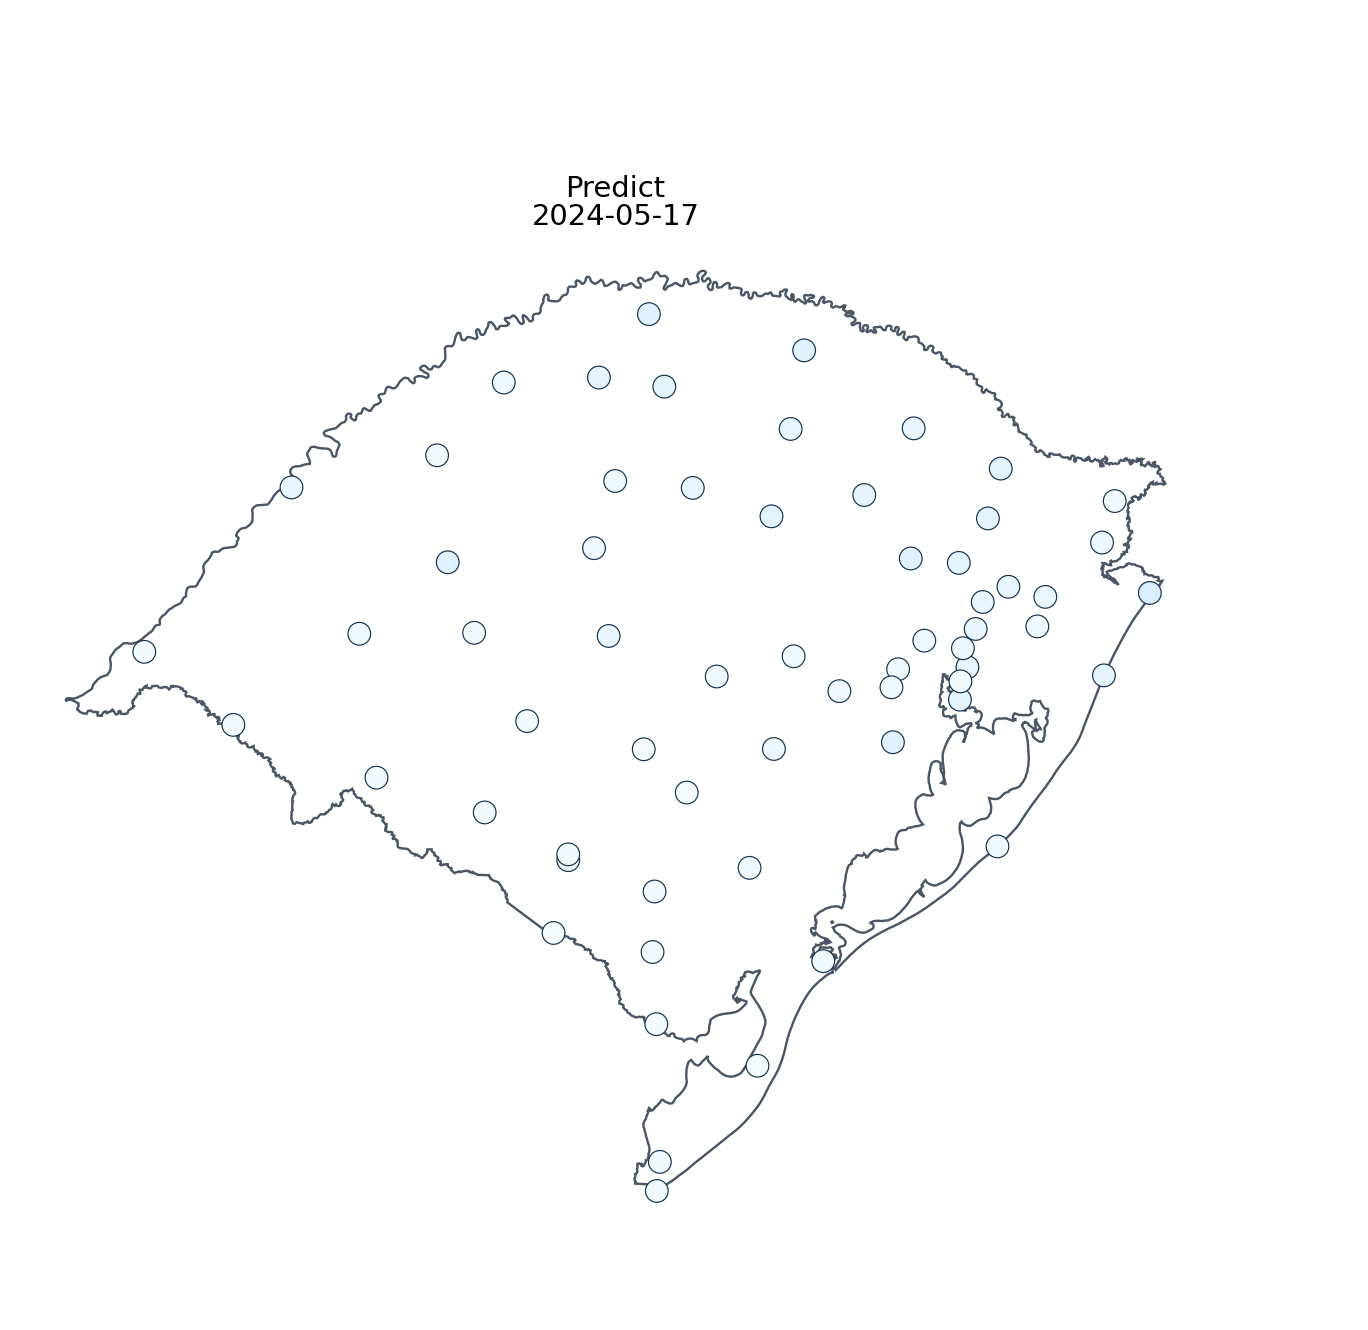
\includegraphics[width=0.48\linewidth]{Predict/frame_028.png}\hfill
    
\includegraphics[width=0.48\linewidth]{Real/frame_028.png}%
  }
  \newframe
  \makebox[\linewidth][c]{%
    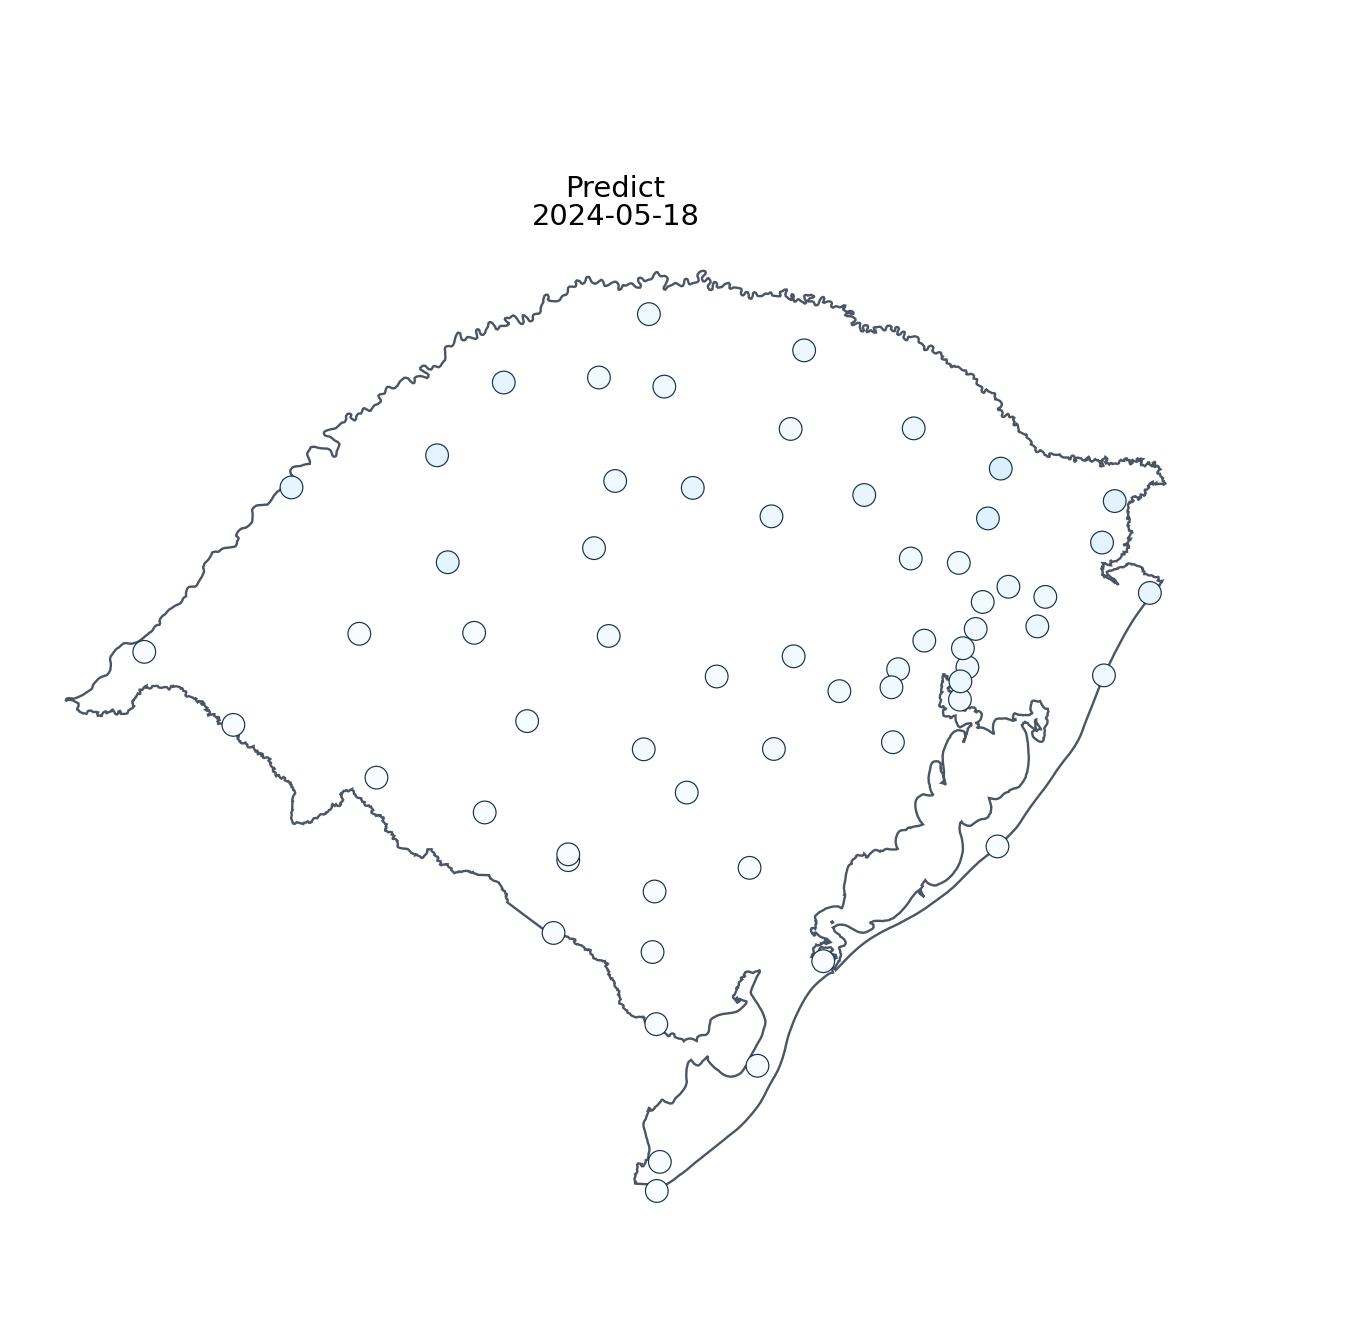
\includegraphics[width=0.48\linewidth]{Predict/frame_029.png}\hfill
    
\includegraphics[width=0.48\linewidth]{Real/frame_029.png}%
  }
  \newframe
  \makebox[\linewidth][c]{%
    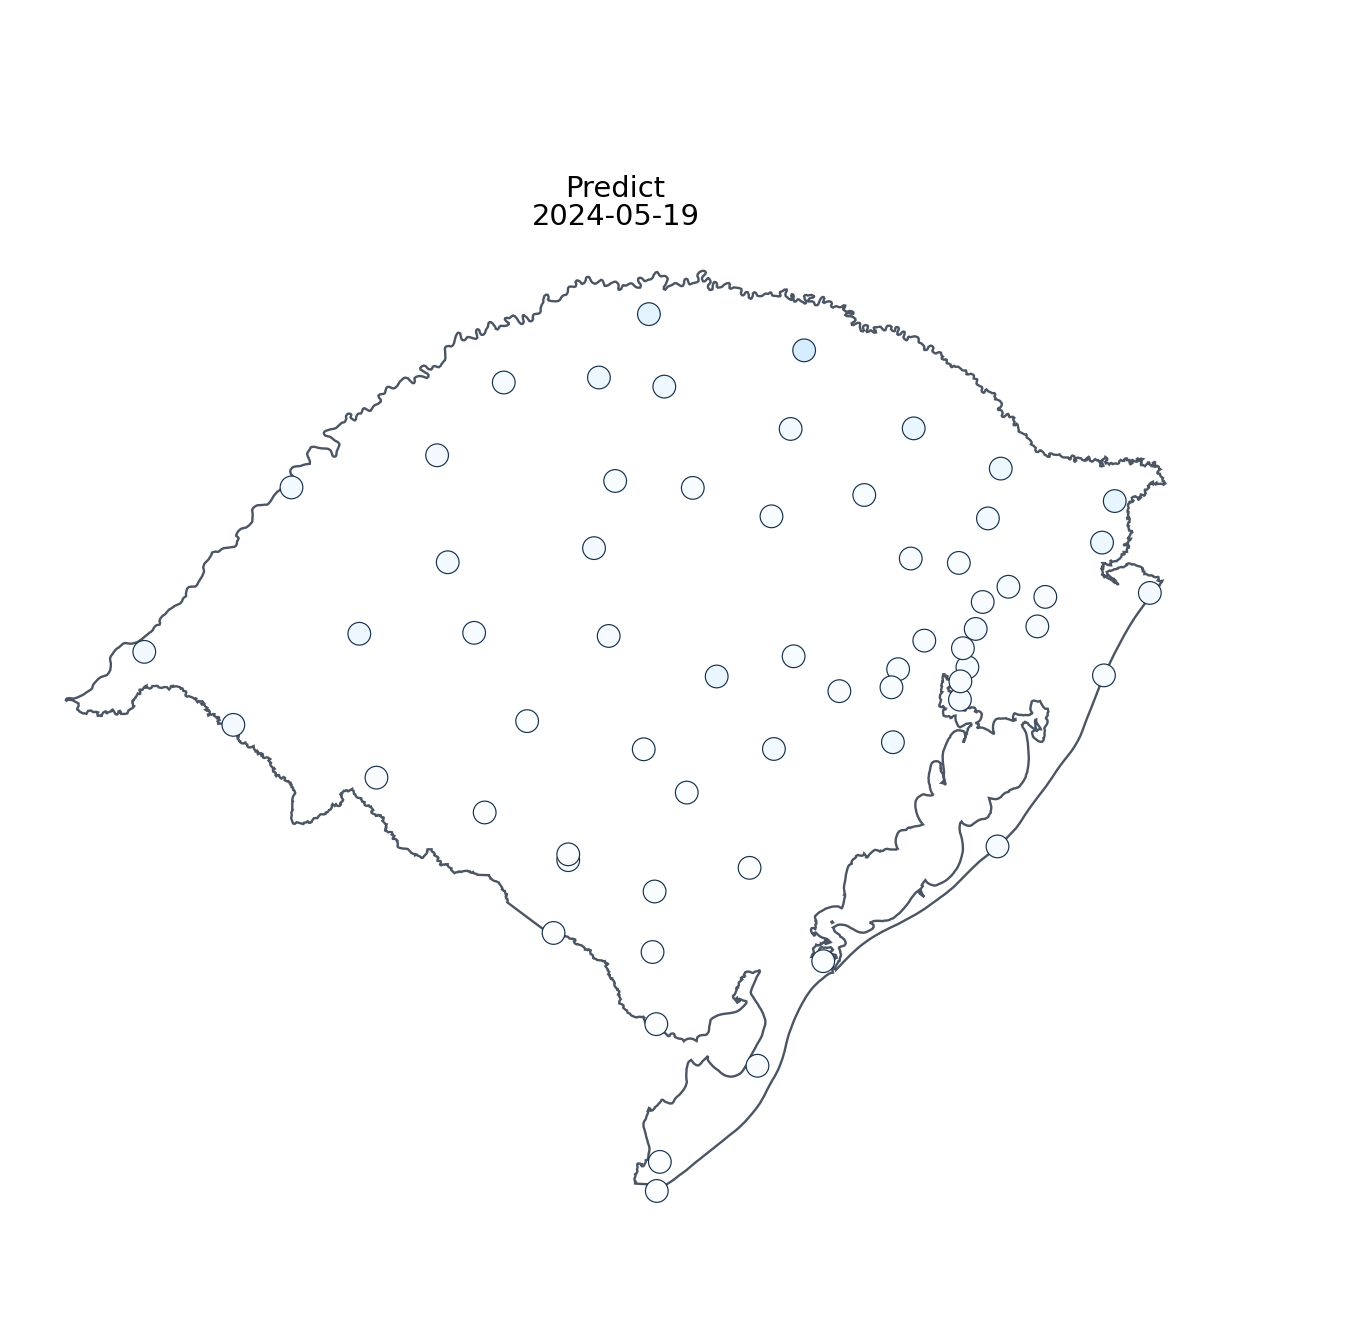
\includegraphics[width=0.48\linewidth]{Predict/frame_030.png}\hfill
    
\includegraphics[width=0.48\linewidth]{Real/frame_030.png}%
  }
  \newframe
  \makebox[\linewidth][c]{%
    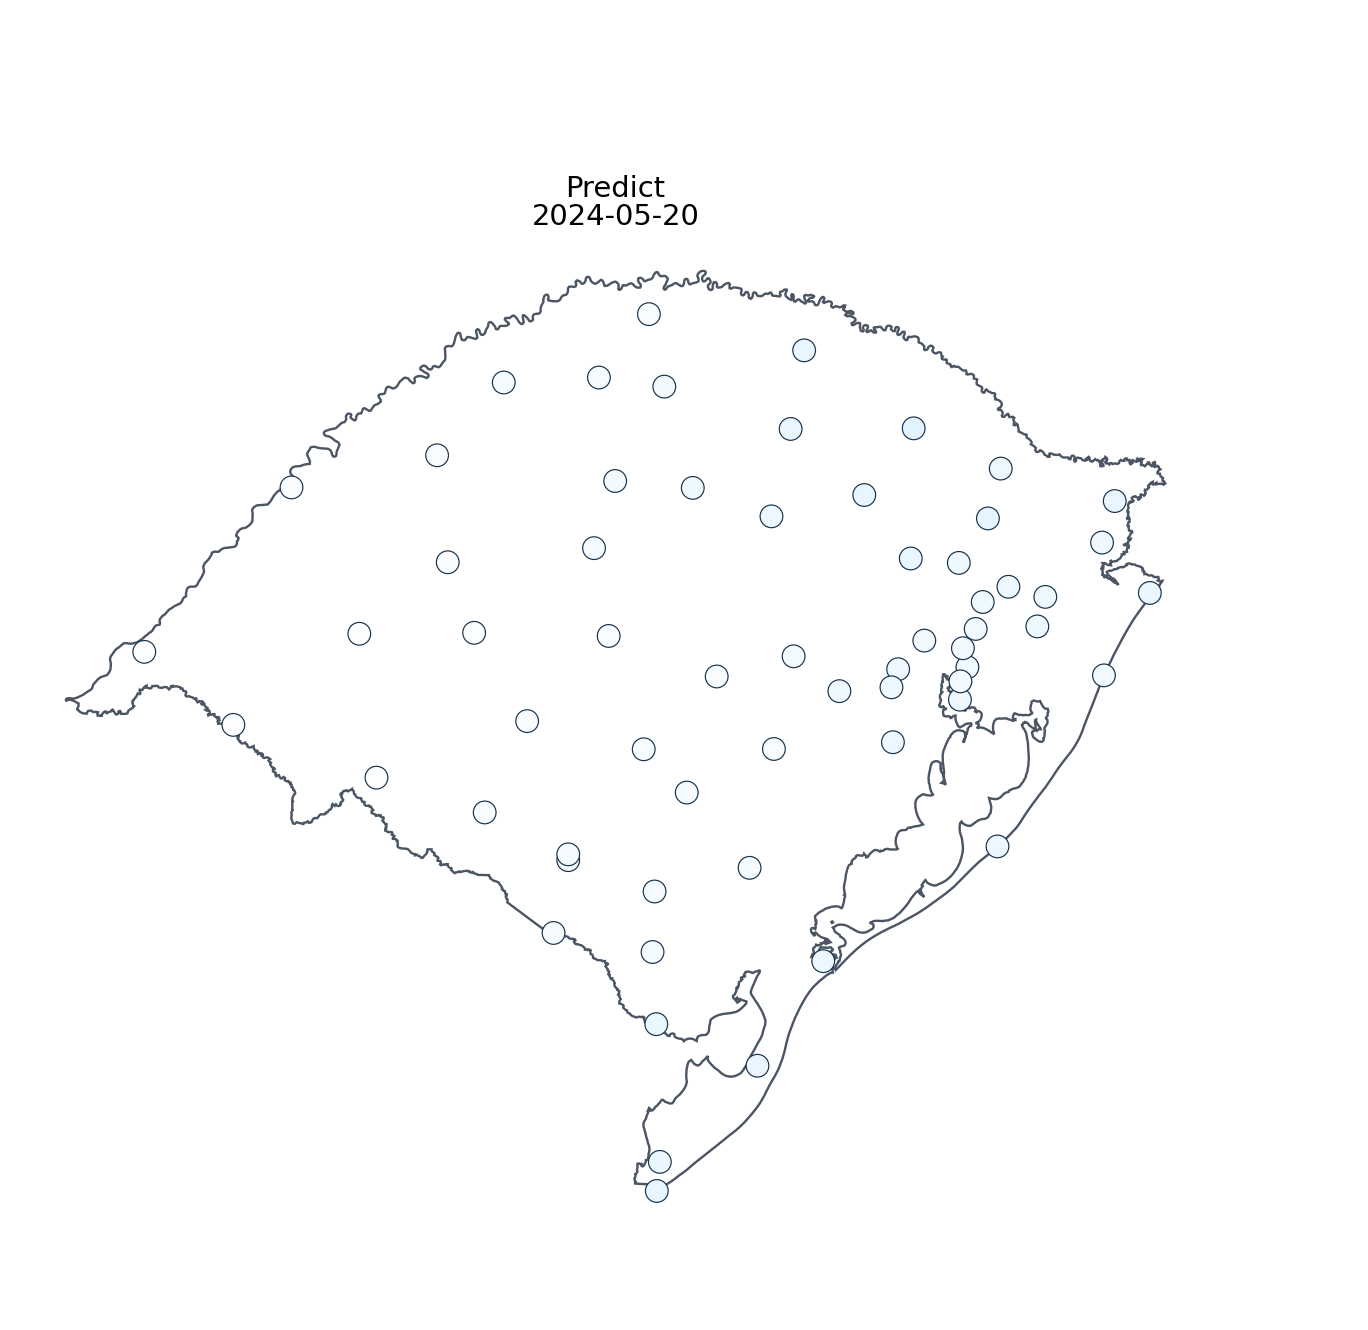
\includegraphics[width=0.48\linewidth]{Predict/frame_031.png}\hfill
    
\includegraphics[width=0.48\linewidth]{Real/frame_031.png}%
  }
\end{animateinline}
\end{minipage}
\end{frame}


\begin{frame}{Learned topology}
    \begin{figure}
        \centering
        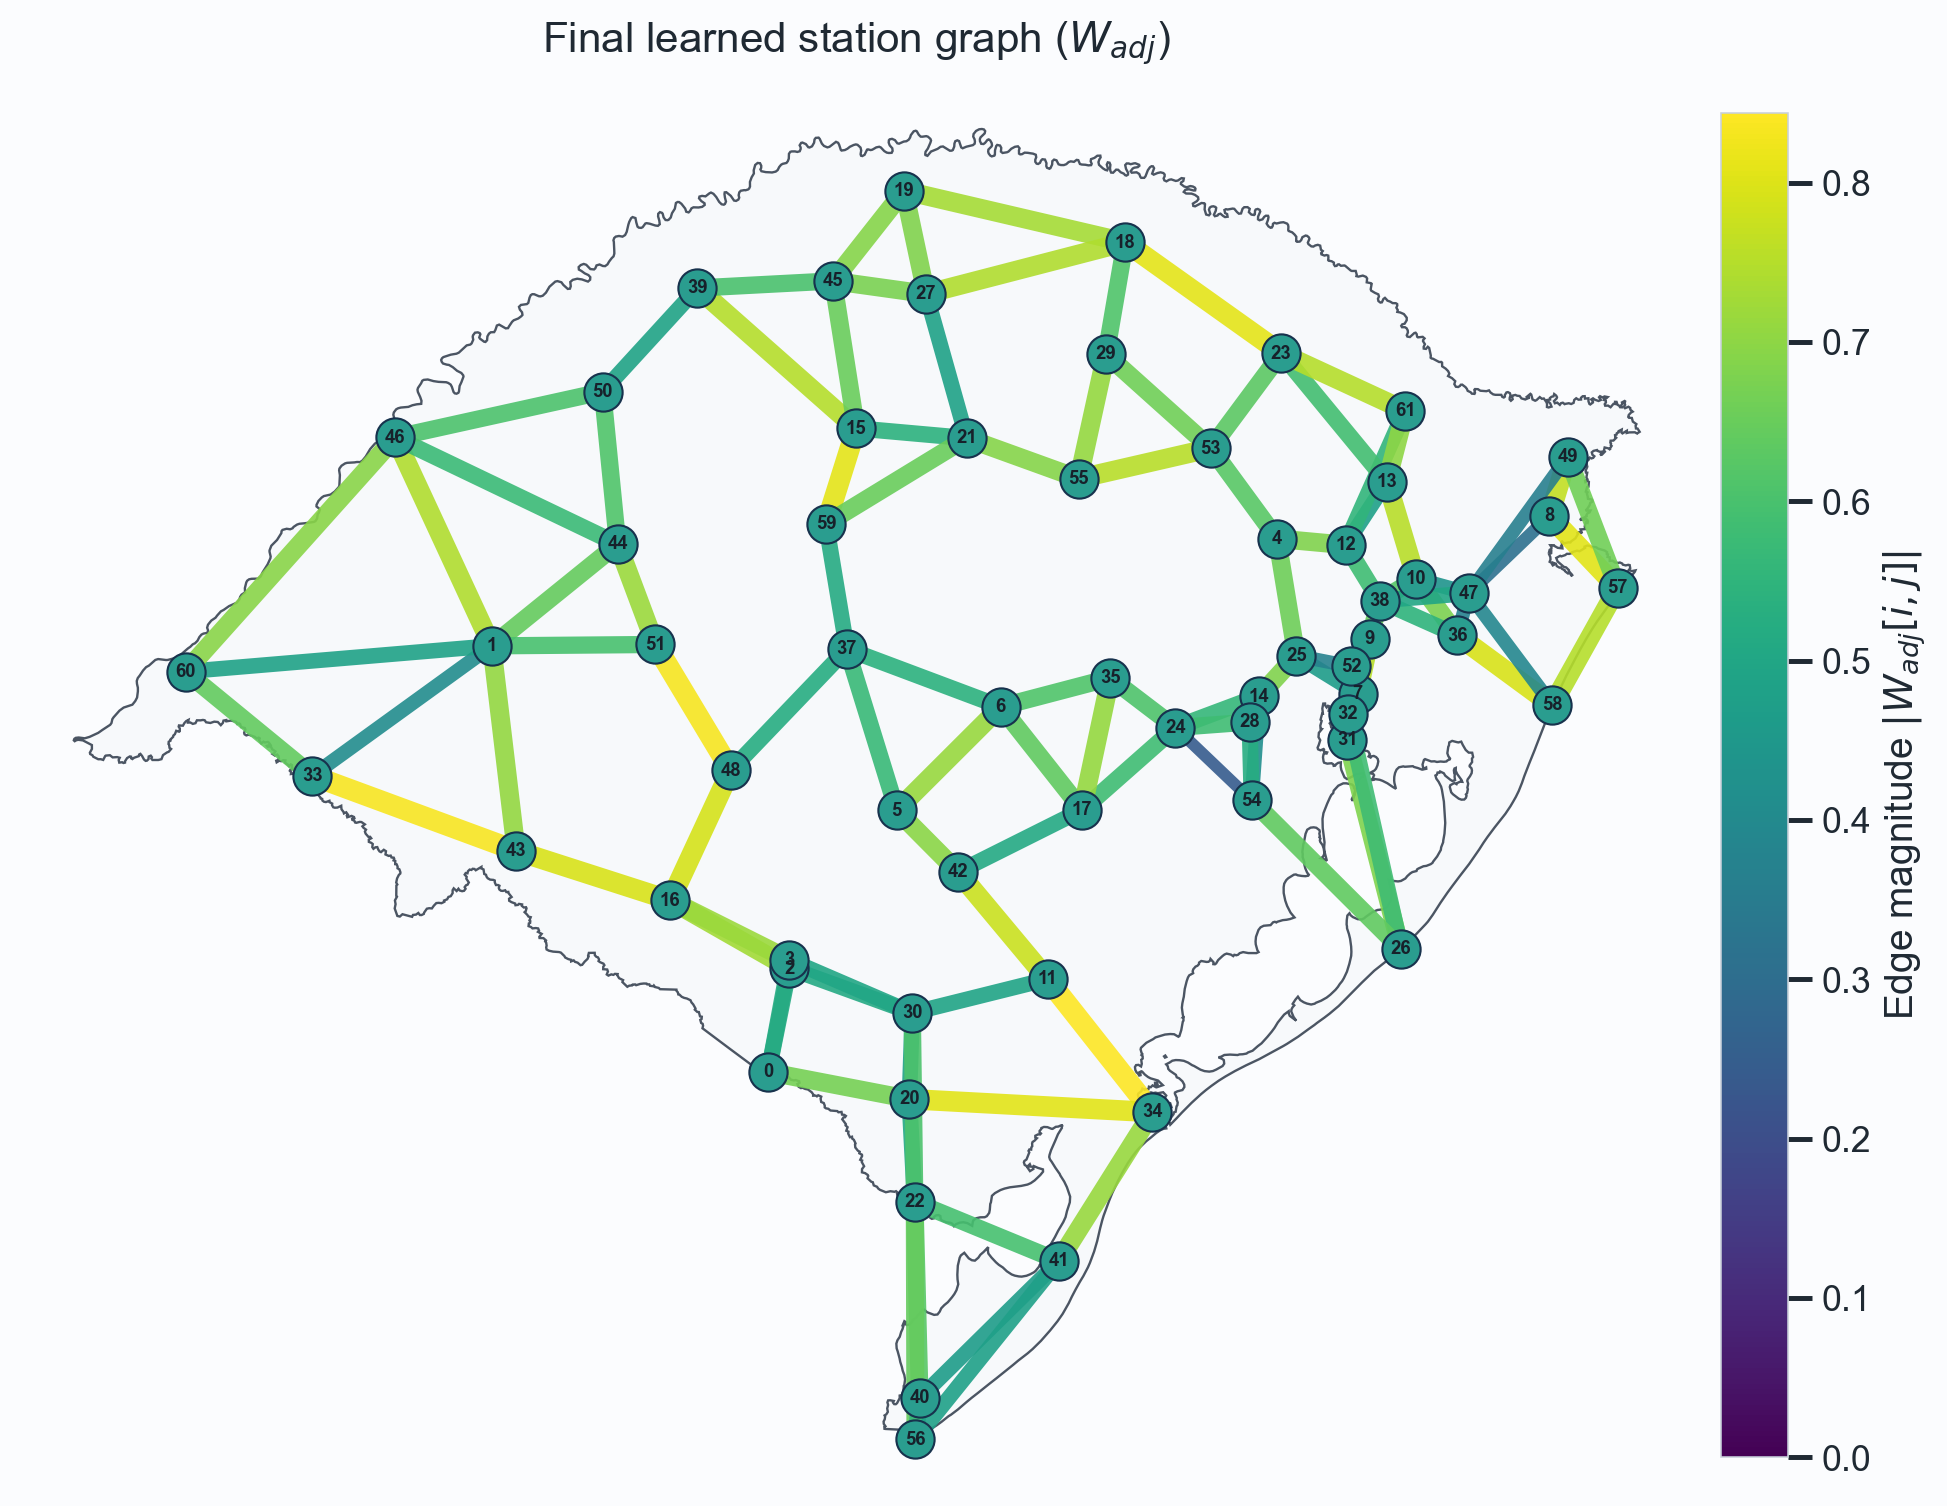
\includegraphics[width=0.65\linewidth]{weighted_graph.png}
    \end{figure}
\end{frame}


\subsection{Future Works}

\begin{frame}{Future Work}
    \begin{itemize}
        \item Improve model performance on extreme precipitation events.
        \item Evaluate alternative spatial modules, such as spectral graph convolutions (ChebConv and CayleyNet).
        \item Evaluate the model using observed precipitation data from INMET stations.
    \end{itemize}
\end{frame}

\begin{frame}

  \begin{center}
  {\Large Thank You! \\ Questions?}
  \end{center}
\end{frame}



\end{document}
